\documentclass[twoside,makeidx]{book}

\usepackage[T1]{fontenc}
\usepackage[utf8]{inputenc}
\usepackage{textcomp}
\usepackage[greek,english,american]{babel} % jonmay for greek unicode characters in titles
\usepackage{enumitem}
\usepackage{xspace}
\usepackage{longtable}
\usepackage{combelow}
%\usepackage{titletoc}
\usepackage{newunicodechar}
%\usepackage[titles]{tocloft}
\usepackage[hidelinks]{hyperref}
\newunicodechar{ș}{\cb{s}}
\newunicodechar{ț}{\cb{t}}
%\titlecontents*{section}[1.5em]{\small}{\thecontentslabel. }{}{, \thecontentspage}[ --- ]
%\setcounter{tocdepth}{1}

%\renewcommand\cftbeforetoctitleskip{-6cm}
%\renewcommand\cftbeforeloftitleskip{-2cm}

%% \usepackage{fontspec,xunicode,xltxtra}
%% \setromanfont[Mapping=tex-text]{Times}
%% \setsansfont[Mapping=tex-text]{Lucida Grande} 
%% \setmonofont{Courier New}

\usepackage{pdfpages}

% set paper size and margins; needs to be adapted for A5 ideally, we
% should have a document class for conference handbooks where A5
% vs. letter-halved is a class option
\usepackage[
  paperheight=8.5in, 
  paperwidth=5.5in, 
  inner=.75in,
  outer=.5in,
  bottom=.75in,
  top=.75in,
  twoside]{geometry}

% Lots of macros
\usepackage[T1]{fontenc}
\PassOptionsToPackage{hyphens}{url}
\usepackage{hyperref}
\usepackage[utf8]{inputenc}
\usepackage{textcomp}
\usepackage{graphicx}
\usepackage{color}
\definecolor{mygray}{gray}{0.75}
\usepackage{colortbl}
\usepackage{fancyhdr}
\usepackage[Bjornstrup]{fncychap}
\usepackage{longtable}
\usepackage{tabularx}
\usepackage{lscape}
\usepackage{array}
\usepackage{calc}
\usepackage{csquotes}
\usepackage[american]{babel}
\usepackage{multicol}
\usepackage{multirow}
\usepackage{times}
\usepackage{helvet}
\usepackage[maxnames=25,minnames=3,babel=hyphen]{biblatex}
\usepackage{bibentry}
\usepackage{setspace}
\usepackage{ifthen}
\usepackage{pstricks}
\usepackage{rotating}
\usepackage{makeidx}
\usepackage{marginnote}
\usepackage{ragged2e}



%\providecommand{\BIBand}{and}

\newcommand{\leftheader}{}  
\newcommand{\rightheader}{} 
\pagestyle{fancy}
  % header spec
  %\renewcommand{\headrule}{{\color[rgb]{0.696,0,0}% 
  \renewcommand{\headrule}{{\color[rgb]{0.132,0.125,.46}% 
    \hrule height 2pt width \headwidth}
    \vspace{1pt}%
    {\color{mygray}%
    \hrule height 1pt width \headwidth
  \vspace{-4pt}}}

  \fancyhf{}				       % clear header contents
  %\fancyhead[LE]{\textit{\nouppercase{\leftmark}}}
  %\fancyhead[RO]{\textit{\nouppercase{\rightmark}}} % define header contents
  \fancyhead[LE]{\textit{\nouppercase{\leftheader}}}
  \fancyhead[RO]{\textit{\nouppercase{\rightheader}}} % define header contents

  % footer spec
  \renewcommand{\footrule}{\hrule width \headwidth height 1mm\vskip\footruleskip}
  \renewcommand{\footruleskip}{0.5\normalbaselineskip}
  \fancyfoot[C]{\thepage}			 %define footer conten

%  \rfoot{\setlength{\unitlength}{1mm} % logo in right part of footer
%  \begin{picture}(0,0)
    %\put(-13,-10){\includegraphics[scale=0.3]{images/conf.jpg}}%
%    \put(-10,-5){\includegraphics[scale=0.2]{images/conf.jpg}}%
%  \end{picture}}

\makeatletter
\renewcommand\chapter{\if@openright\cleardoublepage\else\clearpage\fi %let headers/footers show on pages that start a chapter
                    \global\@topnum\z@
                    \@afterindentfalse
                    \secdef\@chapter\@schapter}

\renewcommand{\chaptermark}[1]{\markboth{#1}{}} % show chapter in header w/o numbering
\renewcommand{\sectionmark}[1]{\markright{#1}{}} % show section in headers w/o numbering

% redefine sections to have a horizontal rule and no numbering
\def\section{\@ifstar\unnumberedsection\numberedsection}
\def\numberedsection{\@ifnextchar[%]
  \numberedsectionwithtwoarguments\numberedsectionwithoneargument}
\def\unnumberedsection{\@ifnextchar[%]
  \unnumberedsectionwithtwoarguments\unnumberedsectionwithoneargument}
\def\numberedsectionwithoneargument#1{\numberedsectionwithtwoarguments[#1]{#1}}
\def\unnumberedsectionwithoneargument#1{\unnumberedsectionwithtwoarguments[#1]{#1}}
\def\numberedsectionwithtwoarguments[#1]#2{
  \ifhmode\par\fi
  \removelastskip
  \vskip 3ex\goodbreak
  \refstepcounter{section}%			   % increment counter
  \begingroup
  \noindent\begin{minipage}{\columnwidth}
  \leavevmode\Large\bfseries\raggedright
%  \thesection\  % leave out numbering
  #2 \par\nobreak
  \vskip -.5em
  \noindent\hrulefill\nobreak
  \end{minipage}
  \endgroup
  \vskip 1ex\nobreak
  \markright{#1}{} % add mark to right (secondary) header
  \addcontentsline{toc}{section}{%
%    \protect\numberline{\thesection}% % leave out number
    #1}%
  }
\def\unnumberedsectionwithtwoarguments[#1]#2{
  \ifhmode\par\fi
  \removelastskip
  \vskip 3ex\goodbreak
  \begingroup
  \noindent\begin{minipage}{\columnwidth}
  \leavevmode\Large\bfseries\raggedright
  #2\par\nobreak
  \vskip -.5em
  \noindent\hrulefill\nobreak
  \end{minipage}
  \endgroup
  \vskip 1ex\nobreak
  \markright{#1}{} % add mark to right (secondary) header
  }

% redefine subsections to have a horizontal rule and no numbering
\def\subsection{\@ifstar\unnumberedsubsection\numberedsubsection}
\def\numberedsubsection{\@ifnextchar[%]
  \numberedsubsectionwithtwoarguments\numberedsubsectionwithoneargument}
\def\unnumberedsubsection{\@ifnextchar[%]
  \unnumberedsubsectionwithtwoarguments\unnumberedsubsectionwithoneargument}
\def\numberedsubsectionwithoneargument#1{\numberedsubsectionwithtwoarguments[#1]{#1}}
\def\unnumberedsubsectionwithoneargument#1{\unnumberedsubsectionwithtwoarguments[#1]{#1}}
\def\numberedsubsectionwithtwoarguments[#1]#2{
  \ifhmode\par\fi
  \removelastskip
  \vskip 3ex\goodbreak
  \refstepcounter{subsection}%			   % increment counter
  \begingroup
  \noindent
  \leavevmode\normalsize\bfseries\raggedright
%  \thesubsection\  % leave out numbering
  #2 \par\nobreak
  \endgroup
  \vskip 1ex\nobreak
  \addcontentsline{toc}{subsection}{%
%    \protect\numberline{\thesubsection}% % leave out number
    #1}%
  }
\def\unnumberedsubsectionwithtwoarguments[#1]#2{
  \ifhmode\par\fi
  \removelastskip
  \vskip 3ex\goodbreak
  \begingroup
  \noindent
  \leavevmode\normalsize\bfseries\raggedright
  #2\par\nobreak
  \endgroup
  \vskip 1ex\nobreak
  }

\makeatother

% Clears to an even-numbered page
\def\clearevenpage{
     \clearpage 
     \ifodd\value{page} \hbox{}\newpage\fi
}

% Clears to the back-cover (for logos)
\def\cleartobackcover{
     \clearpage 
     \ifodd\value{page}\pagestyle{empty}\clearevenpage \else\hbox{}\cleardoublepage\pagestyle{empty}\clearevenpage\fi
}

%\renewcommand{\cleardoublepage}{\clearpage}

% Min: index
\makeindex

%\raggedbottom
%\setlength{\parindent}{0pt}
% Unicode issues
% \DeclareUnicodeCharacter{fi}{fi}

% Min: correct column widths
\newlength{\mycolumnwidth}
\setlength{\mycolumnwidth}{\columnwidth}
\addtolength{\mycolumnwidth}{-2ex}

\renewcommand{\textfraction}{.2}
\renewcommand{\bottomfraction}{.8}

\newenvironment{bio}
               {\begin{figure}[b]
                   \centerline{\rule{.5\linewidth}{.5pt}}\vspace{2ex}
                   \setlength{\parskip}{1ex}\setlength{\parindent}{0ex}}
               {\end{figure}}

\setlength{\parindent}{1em}

\fancypagestyle{emptyheader}
{
  \fancyhf{}
  \fancyfoot[C]{\thepage}
}

\newcommand{\setheaders}[2]{%
  \renewcommand{\leftheader}{#1}%
  \renewcommand{\rightheader}{#2}}
%%%%%%%%%%%%%%%%%%%%%%%%%%%%%%%%%%%%%%%%%%%%%%%%%%
 
% Macros for the production of Conference Handbooks / Program Brochures from
% ACLPUB bundles from the START conference manager.

\newlength{\w}      % width of the space available for paper entries in a
                    % multi-track schedule
\newlength{\tsl}    % with of a time specification in a schedule
\newlength{\en}     % \en-space
%\newlength{\tmplen}

\setlength{\tabcolsep}{.5ex} 

\newenvironment{SingleTrackSchedule}%
{%
  \settowidth{\en}{--}
  \setlength{\w}{\linewidth}%
  \settowidth{\tsl}{$\,$} % temporary abuse of this length measure
  \addtolength{\w}{-2\tsl}%
  \settowidth{\tsl}{00:00}
  \addtolength{\w}{-2\tsl}%
  \addtolength{\w}{-2\tabcolsep}%
  \addtolength{\w}{-1\en}%
  \begin{longtable}{@{}%
      >{\raggedleft}p{\tsl}%
      @{$\,$}%
      p{1\en}%
      @{$\,$}%
      >{\raggedright}p{\tsl}%
      >{\RaggedRight}p{\w}@{}}%
}{%
  \end{longtable}%
}

\newenvironment{TwoTrackSchedule}{
\settowidth{\en}{--}
\setlength{\w}{\linewidth}%
\settowidth{\tsl}{$\,$}
\addtolength{\w}{-2\tsl}%
\settowidth{\tsl}{\footnotesize 00:00am}
\addtolength{\tsl}{2ex}
\addtolength{\w}{-2\tsl}%
\addtolength{\w}{-2\tabcolsep}%
\addtolength{\w}{-1\en}%
\addtolength{\w}{-1cm}%
\renewcommand{\arraystretch}{1.1}
%\setlength{\tmplen}{\tabcolsep}
%\addtolength{\tmplen}{-.5\arrayrulewidth}
\begin{longtable}{@{}|%
    >{\raggedleft}p{\tsl}%
    @{$\,$}%
    p{1\en}%
    @{$\,$}%
    >{\raggedright}%
    p{\tsl}|%
    >{\centering\arraybackslash}p{.5\w}|%
    >{\centering\arraybackslash}p{.5\w}|@{}}%
}{\end{longtable}}

\newenvironment{ThreeTrackSchedule}{
\settowidth{\en}{--}
\setlength{\w}{\linewidth}%
\settowidth{\tsl}{$\,$}
\addtolength{\w}{-2\tsl}%
\settowidth{\tsl}{00:00am}
\addtolength{\tsl}{2ex}
\addtolength{\w}{-2\tsl}%
\addtolength{\w}{-2\tabcolsep}%
\addtolength{\w}{-1\en}%
\addtolength{\w}{-1cm}%
\renewcommand{\arraystretch}{1.1}
%\setlength{\tmplen}{\tabcolsep}
%\addtolength{\tmplen}{-.5\arrayrulewidth}
\begin{longtable}{@{}%
    >{\raggedleft}p{\tsl}%
    @{$\,$}%
    p{1\en}%
    @{$\,$}%
    >{\raggedright}%
    p{\tsl}|%
    >{\centering\arraybackslash}p{.333\w}|%
    >{\centering\arraybackslash}p{.333\w}|%
    >{\centering\arraybackslash}p{.333\w}@{}}%
}{\end{longtable}}

\newenvironment{FourTrackSchedule}{
\settowidth{\en}{--}
\setlength{\w}{\linewidth}%
\settowidth{\tsl}{$\,$}
\addtolength{\w}{-2\tsl}%
\settowidth{\tsl}{00:00am}
\addtolength{\tsl}{2ex}
\addtolength{\w}{-2\tsl}%
\addtolength{\w}{-2\tabcolsep}%
\addtolength{\w}{-1\en}%
\addtolength{\w}{-1cm}%
\renewcommand{\arraystretch}{1.1}
%\setlength{\tmplen}{\tabcolsep}
%\addtolength{\tmplen}{-.5\arrayrulewidth}
\begin{longtable}{@{}|%
    >{\raggedleft}p{\tsl}%
    @{$\,$}%
    p{1\en}%
    @{$\,$}%
    >{\raggedright}%
    p{\tsl}|%
    >{\centering\arraybackslash}p{.25\w}|%
    >{\centering\arraybackslash}p{.25\w}|%
    >{\centering\arraybackslash}p{.25\w}|%
    >{\centering\arraybackslash}p{.25\w}|@{}}%
}{\end{longtable}}

%%%%%%%%%%% BreakTime Macro %%%%%%%%%%%%%%%%%%%%%%%%%%%%%%%%%%%%%%%%%%%%%%
\newcommand{\BreakTime}[4]{%
% adds a gray background to a break or a break-style event
% #1 start time
% #2 end   time
% #3 number of parallel tracks
% #4 label of the break or break-style event
\multicolumn{3}{c}{\cellcolor[gray]{.8}} & 
\multicolumn{#3}{c}{\cellcolor[gray]{.8}} \\[-3ex]\hline 
\bfseries #1 & -- & \bfseries #2 &
\multicolumn{#3}{c|}{\bfseries #4}}
%%%%%%%%%%%%%%%%%%%%%%%%%%%%%%%%%%%%%%%%%%%%%%%%%%%%%%%%%%%%%%%%%%%%%%%%%%

%%%%%%%%%%% PlenaryEvent Macro %%%%%%%%%%%%%%%%%%%%%%%%%%%%%%%%%%%%%%%%%%%%%%
\newcommand{\PlenaryEvent}[4]{%
% event with nothing else going on in parallel
\bfseries #1 & -- & \bfseries #2 &
\multicolumn{#3}{>{\centering\arraybackslash}p{\w}|@{}}{\bfseries #4}}
%%%%%%%%%%%%%%%%%%%%%%%%%%%%%%%%%%%%%%%%%%%%%%%%%%%%%%%%%%%%%%%%%%%%%%%%%%

%%%%%%%%%%% SessionHeader Macro %%%%%%%%%%%%%%%%%%%%%%%%%%%%%%%%%%%%%%%%%%%%%%
\newcommand{\SingleTrackSessionHeader}[3]{%
% event with nothing else going on in parallel
\ifthenelse{\equal{{#1}}{{}}}{&}{#1 & -- } & #2 
\ifthenelse{\equal{#1}{{}}}{}{\hfill}
&\multicolumn{1}{>{\raggedright\arraybackslash}m{\w}}{\bfseries #3}}
%%%%%%%%%%%%%%%%%%%%%%%%%%%%%%%%%%%%%%%%%%%%%%%%%%%%%%%%%%%%%%%%%%%%%%%%%%

% insert references to the page ranges 
\newcommand{\ppp}[1]{pp. \pageref{#1start}--\pageref{#1end}}

% #1 = last name
% #2 = last name (initials)
% #3 = first name
% #4 = first name (initials)
% #5 = name prefix, a.k.a. 'von part'
% #6 = name prefix (initials)
% #7 = name affix, a.k.a. 'junior part'
% #8 = name affix (initials)


% the following code requires the biblatex package
\DeclareNameFormat{authorswithinitials}{%
  % name format that prints the list of authors with initals
  \ifcase\value{uniquename}%
%%%    \usebibmacro{name:given-family}{#1}{#4}{#5}{#7}%
    \nameparts{#1}%
      \usebibmacro{name:given-family}
        {\namepartfamily}
        {\namepartgiveni}
        {\namepartprefix}
        {\namepartsuffix}%
  \or
    \ifuseprefix
    \nameparts{#1}%
      \usebibmacro{name:given-family}
        {\namepartfamily}
        {\namepartgiveni}
        {\namepartprefix}
        {\namepartsuffixi}%
      \usebibmacro{name:given-family}
        {\namepartfamily}
        {\namepartgiveni}
        {\namepartprefixi}
        {\namepartsuffixi}%
%%%      {\usebibmacro{name:given-family}{#1}{#4}{#5}{#8}}
%%%      {\usebibmacro{name:given-family}{#1}{#4}{#6}{#8}}%
  \or
%%%    \usebibmacro{name:given-family}{#1}{#4}{#5}{#7}%
\nameparts{#1}%
      \usebibmacro{name:given-family}
        {\namepartfamily}
        {\namepartgiveni}
        {\namepartprefix}
        {\namepartsuffix}%
  \fi
  \usebibmacro{name:andothers}}

\DeclareNameFormat{authorlastnames}{%
  % name format that prints the list of author last names
  \ifcase\value{uniquename}%
%%%    \usebibmacro{name:family}{#1}{#4}{#5}{#7}%
\nameparts{#1}%
      \usebibmacro{name:given-family}
        {\namepartfamily}
        {\namepartgiveni}
        {\namepartprefix}
        {\namepartsuffix}%
  \or
    \ifuseprefix
\nameparts{#1}%
      \usebibmacro{name:given-family}
        {\namepartfamily}
        {\namepartgiveni}
        {\namepartprefix}
        {\namepartsuffixi}%
\nameparts{#1}%
      \usebibmacro{name:given-family}
        {\namepartfamily}
        {\namepartgiveni}
        {\namepartprefixi}
        {\namepartsuffixi}%
%%%      {\usebibmacro{name:family}{#1}{#4}{#5}{#8}}
%%%      {\usebibmacro{name:family}{#1}{#4}{#6}{#8}}%
  \or
\nameparts{#1}%
      \usebibmacro{name:given-family}
        {\namepartfamily}
        {\namepartgiveni}
        {\namepartprefix}
        {\namepartsuffix}%
%%%    \usebibmacro{name:family}{#1}{#4}{#5}{#7}%
  \fi
  \usebibmacro{name:andothers}}

\DeclareNameFormat{fullauthornames}{%
  % name format that prints the list of authors with full author names
  \ifcase\value{uniquename}%
  \nameparts{#1}%
      \usebibmacro{name:given-family}
        {\namepartfamily}
        {\namepartgiven}
        {\namepartprefix}
        {\namepartsuffix}%
%%%    \usebibmacro{name:given-family}{#1}{#3}{#5}{#7}%
    \or
    \ifuseprefix
\nameparts{#1}%
      \usebibmacro{name:given-family}
        {\namepartfamily}
        {\namepartgiven}
        {\namepartprefix}
        {\namepartsuffixi}%
\nameparts{#1}%
      \usebibmacro{name:given-family}
        {\namepartfamily}
        {\namepartgiven}
        {\namepartprefixi}
        {\namepartsuffixi}%
%%%        {\usebibmacro{name:given-family}{#1}{#3}{#5}{#8}}
%%%        {\usebibmacro{name:given-family}{#1}{#3}{#6}{#8}}%
  \or
\nameparts{#1}%
      \usebibmacro{name:given-family}
        {\namepartfamily}
        {\namepartgiven}
        {\namepartprefix}
        {\namepartsuffix}%
%%%  \usebibmacro{name:given-family}{#1}{#3}{#5}{#7}%
  \fi
  \usebibmacro{name:andothers}}

% insert the list of authors with first name initials
\DeclareCiteCommand{\citeauthorslastnamesonly}{%
  \boolfalse{citetracker}%
  \boolfalse{pagetracker}%
  \usebibmacro{prenote}%
}{\ifciteindex{\indexnames{labelname}}{}%
  \printnames[authorlastnames]{labelname}%
}{\multicitedelim}{\usebibmacro{postnote}}

% insert the list of authors with first name initials
\DeclareCiteCommand{\citeauthorswithinitials}{%
  \boolfalse{citetracker}%
  \boolfalse{pagetracker}%
  \usebibmacro{prenote}%
}{\ifciteindex{\indexnames{labelname}}{}%
  \printnames[authorswithinitials]{labelname}%
}{\multicitedelim}{\usebibmacro{postnote}}
  
% insert the list of authors with full names
\DeclareCiteCommand{\citefullauthornames}{%
  \boolfalse{citetracker}%
  \boolfalse{pagetracker}%
  \usebibmacro{prenote}%
}{%\ifciteindex{\indexnames{labelname}}{}%
  \indexnames{labelname}%
  \printnames[fullauthornames]{labelname}%
}{\multicitedelim}{\usebibmacro{postnote}}
                     
\DeclareFieldFormat[inproceedings]{citetitle}{#1}

\newcommand{\paperauthor}[1]{{\em #1}}
\newcommand{\papertitle}[1]{\citetitle{#1}}

% insert an entry into a multi-track schedule cell
\newcommand{\paperentry}[1]{%
  \renewcommand{\baselinestretch}{.8}%
  \setlength{\parindent}{0pt}%
    \begin{small}%
      \parbox[t]{\linewidth}{%
        {\em \papertitle{#1}}
        \vspace{.5ex}}\par%
      \vfill
      \parbox[b]{\linewidth}{\raggedright%
        \paperauthor{\citeauthorslastnamesonly{#1}}%
        %% \mbox{}~\dotfill~ {\bfseries p.~\pageref{#1}}
        }%
    \end{small}%
}

\newcommand{\sempaperentry}[1]{%
  &&$\bullet$&
  \parbox[t]{\linewidth}{\raggedright\papertitle{#1}\newline
  {\itshape\paperauthor{\citefullauthornames{#1}}}
\mbox{}~\dotfill~\pageref{#1}}}

\newcommand{\atpaperentry}[2]{%
  \footnotesize\parbox[t]{\linewidth}{\noindent%
    \makebox[0pt][r]{#1\hspace*{\tabcolsep}}{%
      \paperauthor{\citeauthorswithinitials{#2}}}:
    \papertitle{#2}\mbox{}~\dotfill{p.~\pageref{#2}\par}}}

% insert an entry into a poster session index
\newcommand{\posterentry}[1]{%
  \renewcommand{\baselinestretch}{1.2}%
  \settowidth{\w}{\bfseries p.~\pageref{#1}}%
  \addtolength{\w}{1em}%
  \parbox[t]{\linewidth-\w}{\noindent\raggedright{\bfseries\papertitle{#1}}%
    \linebreak[0]\ {---~{\paperauthor{\citeauthorswithinitials{#1}}}}\mbox{}~\dotfill\makebox[0pt][l]%
    {\makebox[\w][r]{\bfseries p.~\pageref{#1}}}\vspace{1em}\par}}

% insert an abstract into a list of abstracts (for posters, no time needed)
\newcommand{\posterabstract}[1]{%
  \noindent%
  \begin{minipage}{\linewidth}%
    \label{#1}%
          {\bfseries\normalsize\papertitle{#1}}\\
          \normalsize\paperauthor{\citefullauthornames{#1}}
  \end{minipage}\vspace{1mm}\\\nopagebreak%
  \noindent{\small\input{auto/abstracts/#1}}\par}

% insert an abstract into a list of abstracts
\newcommand{\paperabstract}[5]{%
  % #1 day
  % #2 time
  % #3 session title
  % #4 location
  % #5 paper id
  \noindent%
  \begin{minipage}{\linewidth}%
    \label{#5}%
      %\rule{\linewidth}{1pt}\linebreak
          {\bfseries\normalsize\papertitle{#5}} \\
          \hfill\normalsize\paperauthor{\citefullauthornames{#5}}
%      {\small #1 #2 --- #4}\vspace{.5ex}\\
          \hfill {\small #2}
%    \parbox[t]{.8\linewidth}{\centering
%      {\bfseries\papertitle{\citetitle{#5}}}\linebreak
%      \paperauthor{\citefullauthornames{#5}}}%
%    \parbox[t]{.2\linewidth}{\raggedleft\small%
%      #1\linebreak #2\linebreak #4}\par\nopagebreak
  %% \begin{center}\label{#5}%
  %%   \sloppy\hyphenpenalty=0%
  %%   %{\small --- Session: #3 --- \vspace{.5em}}\linebreak		% Redundant info? - B
  %%   {\bfseries \citetitle{#5}} \vspace{.5em}\linebreak
  %%   {\itshape    \citefullauthornames{#5}}%\vspace{.5em}\linebreak	% Reduce space between header and abstract - B
  %%   %#1 #2 --- #4\linebreak 						% Redundant info? - B
  \end{minipage}\vspace{1mm}\\\nopagebreak%
  \noindent{\small\input{auto/abstracts/#5}}\par}

\newcommand{\TutorialCoverPage}[4]{%
\vspace*{.25in}
% #1 Tutorial Number
% #2 Tutorial Title
% #3 Tutorial Presenter
% #4 Tutorial Presenter Information
%\begin{minipage}{\linewidth}
\begin{centering}
\includegraphics[height=7.5cm,clip=true]{content/fmatter/conference-logo.eps}\\

\vspace{.5cm}

{\Large
The 2012 Conference of the \linebreak
North American Chapter of the \linebreak
Association for Computational Linguistics: \linebreak
Human Language Technologies}\par

\vspace{3cm}

%\begin{tabular}{@{}>{\centering\arraybackslash}p{.7\linewidth}@{}}
\centerline{\huge\bfseries Tutorial~#1\vspace{.25em}}
{\Large Tutorial Notes}\\

\vspace{1cm}

\begin{minipage}{.7\linewidth}
\centering\Large%\setstretch{1.1}
{\bfseries#2}
\end{minipage}

\vfill

{\itshape\Large #3}\\[.5em]
{#4}\\
\vspace{1cm}

{June 3, 2012}\\
{Montr\'{e}al, Queb\'{e}c, Canada}\\\end{centering}
%\end{minipage}
\clearpage}

\newcommand{\STARSEM}{$^\ast$SEM}

\newcommand{\nix}{\cellcolor{mygray}}
% used for the room occupation tables in the local information section

\newcommand{\mrup}[2]{\multirow{#1}{*}{%
%\rotatebox[origin=c]{90}{#2}}%
\begin{sideways}#2\end{sideways}%
}}

\newcommand{\PaperInSchedule}[4][false]{%
  % #1 (optional) with or without a \pageref to the abstract
  % #2 start time (can be empty)
  % #3 end time (can be empty)
  % #4 paper id
  \ifthenelse{\equal{{#2}}{{}}}{&&\hfill}{#2&--&} % ... start time
  \ifthenelse{\equal{{#3}}{{}}}{$\bullet$}{#3}    %   ... end time
    & \parbox[t]{\linewidth}{\raggedright\papertitle{#4}\newline
      {\paperauthor{\citefullauthornames{#4}}}%
      \ifthenelse{\equal{#1}{true}}{\mbox()~\dotfill~\pageref{#4}}}}

\newcommand{\ScheduleItem}[4][false]{%
  % #1 (optional) with or without a \pageref to the abstract
  % #2 start time (can be empty)
  % #3 end time (can be empty)
  % #4 paper id
  \ifthenelse{\equal{{#2}}{{}}}{&&\hfill}{#2&--&} % ... start time
  \ifthenelse{\equal{{#3}}{{}}}{$\bullet$}{#3}    %   ... end time
    & \parbox[t]{\linewidth}{\raggedright\papertitle{#4}\newline
      {\paperauthor{\citefullauthornames{#4}}}%
      \ifthenelse{\equal{#1}{true}}{\mbox()~\dotfill~\pageref{#4}}}}

\newenvironment{singledaywsprogram}[5]{%
% #1 worshop id
% #2 workshop number
% #3 workshop title
% #4 workshop day
% #5 workshop venue
\section{\textbf{W~#2:} #3}\label{#1}

\begin{center}
{\bfseries\Large #4}\vspace{1em}\par
{\itshape Venue:} #5\vspace{0.75em}\par
{\large\bfseries Program\vspace{0.75em}}\par
\setlength{\w}{\linewidth}
\begin{SingleTrackSchedule}}%
{\end{SingleTrackSchedule}\end{center}}

%% WORKSHOP SCHEDULE %%%%%%%%%%%%%%%%%%%%%%%%%%%%%%%%%%%%%%%%%%%%

%\newlength{\wsscheduleindentation}
%\newlength{\wsschedulelabelwidth}
\newenvironment{wsschedule}[5]{%
  % #1 workshop title
  % #2 workshop number
  % #3 workshop label
  % #4 workshop paper ID
  % #5 workshop location
  %\addcontentsline{toc}{section}{{{\bfseries W~#2:} #4}}

  %\addcontentsline{toc}{section}{{{\bfseries W~#2:} 
  %    \ifthenelse{\equal{#1}{none}}{#4}{#1}}}

  % For workshops numbered 0, don't prepend W0 on the contents page
  \clearpage
  \ifthenelse{\equal{#2}{0}}
%%             {\section{\textbf{#1}}}
             {\section{#1}}
%%
%% For ACL 2017, we do not show the Wx prefix and instead only show the title
%%             {\section[{\bfseries W#2:} #1]{{\bfseries Workshop #2:} #1}}
             {\section{#1}}
             %% {{\addcontentsline{toc}{section}{{#1}}}}
             %% {{\addcontentsline{toc}{section}{{{\bfseries W#2:} #1}}}}

  \markboth{}{}
  \label{#3}
  \begin{center}
%    {\huge{\Large Workshop #2:}\vspace{.5ex}\\
    %% {\Large
    %%   \ifthenelse{\equal{#2}{0}}{{}}{{\huge{Workshop #2:\\\vspace{.5ex}}}}
    %%   #1\par}
    {\ifthenelse{\equal{#4}{0}}{{}}{{Organizers: \paperauthor{\citefullauthornames{#4}}}\par}}
    {\large Venue: #5 \vspace{2em}}\\
    %% {\huge Workshop Program\vspace{1ex}}
  \end{center}
  \markright{{\bfseries W~#2:} #1}{}%
  \begin{list}{{}}{%
      \settowidth{\labelwidth}{\bfseries 12:00pm--12:00pm}
      \setlength{\labelsep}{1ex}
      \setlength{\topsep}{0pt}
      \setlength{\parsep}{0pt}
      \setlength{\listparindent}{0pt}
      \setlength{\itemsep}{.5ex}
      \setlength{\rightmargin}{0pt}
      \setlength{\leftmargin}{\labelwidth}
      \addtolength{\leftmargin}{\labelsep}}
}{\end{list}}

\newcounter{WorkshopCounter}

\newenvironment{tutorial}[4]{%
  \stepcounter{TutorialCounter}
  % #1 short title
  % #2 tutorial bibtex ID
  % #3 date and time
  % #4 location

  % Cannot get \papertitle to expand
  \section[\textbf{T\theTutorialCounter:} {#1}]{Tutorial \theTutorialCounter}
  \begin{center}
    \begin{Large}
      \bfseries \papertitle{#2}\\ \vspace{2em}\par
    \end{Large}
    {\itshape \tutorialauthors{#2}}\vspace{1em}\par
    #3 \vspace{1em}\\
    #4
  \end{center}}

\newcounter{TutorialCounter}

\newcommand{\tutorialauthors}[1]{
    \paperauthor{\citefullauthornames{#1}}}

\newcommand{\wspaperentry}[1]{
  \parbox[t]{\linewidth}{\raggedright\papertitle{#1}\newline
    \paperauthor{\citefullauthornames{#1}}}}

\newcommand{\sessionchair}[2]{
  \emph{Chair: #1 #2}\par\index{#2, #1}}

\newcommand{\papertitleandauthor}[1]{
  {\bfseries \papertitle{#1}}\\
  \paperauthor{\citefullauthornames{#1}}}

\newcommand{\papertableentry}[1]{
  \scriptsize
  {\papertitle{#1}}\newline
  {\paperauthor{\citeauthorslastnamesonly{#1}}}}

\newenvironment{SessionOverview}[7]{
  \section[#1]{#1 Overview -- #2}
  \setheaders{#1}{#2}
  \begin{center}
    \righthyphenmin2
    \sloppy
    \begin{tabular}{>{\RaggedRight}p{0.8in}|>{\RaggedRight}p{0.8in}|>{\RaggedRight}p{0.8in}|>{\RaggedRight}p{0.8in}|>{\RaggedRight}p{0.8in}}
      \bf Track A & \bf Track B & \bf Track C & \bf Track D & \bf Track P \\
      \it #3 & \it #4 & \it #5 & \it #6 & \it #7 \\
      \TrackALoc & \TrackBLoc & \TrackCLoc & \TrackDLoc & \TrackPLoc \\
      \hline\hline}
{\end{tabular}\end{center}}

\newenvironment{TwoSessionOverview}[4]{
  \section[#1]{#1 Overview -- #2}
  \setheaders{#1}{#2}
  \begin{center}
    \righthyphenmin2
    \sloppy
    \begin{tabular}{|>{\RaggedRight}p{2.0in}|>{\RaggedRight}p{2.0in}|}
      \hline
      \bf Track A & \bf Track B \\\hline
      \it #3 & \it #4 \\
      \TrackALoc & \TrackBLoc \\
      \hline\hline}
{\hline\end{tabular}\end{center}}

\newenvironment{ThreeSessionOverview}[5]{
  \section[#1]{#1 Overview -- #2}
  \setheaders{#1}{#2}
  \begin{center}
    \righthyphenmin2
    \sloppy
    \begin{tabular}{|>{\RaggedRight}p{1.3in}|>{\RaggedRight}p{1.3in}|>{\RaggedRight}p{1.3in}|}
      \hline
      \bf Track A & \bf Track B & \bf Track C \\\hline
      \it #3 & \it #4 & \it #5 \\
      \TrackALoc & \TrackBLoc & \TrackCLoc \\
      \hline\hline}
{\hline\end{tabular}\end{center}}

\newcommand{\daydate}{DAY, DATE}
\newcommand{\daydateyear}{DAY, DATE, YEAR}
\newcommand{\setdaydateyear}[3]{
  \renewcommand{\daydateyear}{#1, #2, #3\xspace}
  \renewcommand{\daydate}{#1, #2\xspace}}
    

%% defines macros for event venues

% ACL 2017 Venues
 \newcommand{\TrackALoc}{\mbox{Empire A}}
 \newcommand{\TrackBLoc}{\mbox{Empire B}}
 \newcommand{\TrackCLoc}{\mbox{Empire C}}
 \newcommand{\TrackDLoc}{\mbox{Empire D}}
 \newcommand{\TrackPLoc}{\mbox{Elite Hall B}}
 \newcommand{\TrackFLoc}{\mbox{Not a real location}}
 \newcommand{\TrackGLoc}{\mbox{Also Not a real location}}

\newcommand{\UnknownLoc}{TBD}
% \newcommand{\BestLocA}{\mbox{Salons A/B/C}}
% \newcommand{\BestLocB}{\mbox{Salons D/E/F}}

\newcommand{\WelcomeReceptionLoc}{\mbox{TODO}}
\newcommand{\BreakfastLoc}{\mbox{Empire Foyer}}
\newcommand{\BreakLoc}{\BreakfastLoc}
\newcommand{\RegistrationLoc}{\BreakfastLoc}
\newcommand{\PosterSessionLoc}{\mbox{Elite Hall B}}
\newcommand{\SrwLoc}{\PosterSessionLoc}
\newcommand{\PosterLoc}{\PosterSessionLoc}
\newcommand{\DemoLoc}{\PosterSessionLoc}
\newcommand{\PlenaryLoc}{\mbox{Empire Ballroom}}

% Tutorials
\newcommand{\TutLocA}{\mbox{Bolden 5}}
\newcommand{\TutLocB}{\mbox{Bolden 6}}
\newcommand{\TutLocC}{\mbox{Strand 13}}
\newcommand{\TutLocD}{\mbox{Bolden 5}}
\newcommand{\TutLocE}{\mbox{Bolden 6}}
\newcommand{\TutLocF}{\mbox{Strand 13}}

% Main conference
\newcommand{\CoffeeLoc}{\mbox{Empire Foyer}}
\newcommand{\SocialEventLoc}{Blaine Kern's Mardi Gras World}
\newcommand{\BusinessMeetingLoc}{\mbox{Empire Ballroom}}
\newcommand{\InvitedLoc}{\PlenaryLoc}
\newcommand{\ClosingSessionLoc}{\PlenaryLoc}
\newcommand{\LifetimeAchievementSessionLoc}{\PlenaryLoc}

% Workshop locations
  \newcommand{\WShopLocWiNLP}{\mbox{Strand 12}}
  \newcommand{\WShopLocSemEval}{\mbox{Strand 10}}
   \newcommand{\WShopLocStarSEM}{\mbox{Strand 12B}}
  \newcommand{\WShopLocGenDeep}{\mbox{Strand 11}}
  \newcommand{\WShopLocBEA}{\mbox{Strand 12A}}
   \newcommand{\WShopLocEthicsNLP}{\mbox{Bolden 1}}
  \newcommand{\WShopLocCLPsych}{\mbox{Bolden 5}}
  \newcommand{\WShopLocSemBEaR}{\mbox{Bolden 4}}
  \newcommand{\WShopLocStyleVar}{\mbox{Bolden 3}}
  \newcommand{\WShopLocSCLeM}{\mbox{Bolden 6}}
   \newcommand{\WShopLocTextGraphs}{\mbox{Bolden 1}}
   \newcommand{\WShopLocFigLang}{\mbox{Bolden 2}}
   \newcommand{\WShopLocPEOPLES}{\mbox{Strand 11}}
   \newcommand{\WShopLocCRAC}{\mbox{Bolden 3}}
   \newcommand{\WShopLocSpLU}{\mbox{Bolden 4}}




%%%
% Unclear if these will be used
%%%

% \newcommand{\StarSEMLoc}{\mbox{\color{red}TBC}}
% \newcommand{\SemEvalLoc}{\mbox{\color{red}TBC}}
% \newcommand{\StudentLunchLoc}{\mbox{\color{red}TBC}}
% \newcommand{\OMMLoc}{\PlenaryLoc}
% \newcommand{\BanquetLoc}{\mbox{\color{red}TBC}}
% \newcommand{\LunchLoc}{\mbox{}}
% \newcommand{\BusinessLoc}{\BusinessMeetingLoc}    % business meeting
% \newcommand{\NaaclLoc}{\BusinessMeetingLoc}    % business meeting
% \newcommand{\WelcomeLoc}{\PlenaryLoc}
% \newcommand{\OneLoc}{\PlenaryLoc}  % one minute madness
    % macros for event locations
% define macros for session titles here
\newcommand{\DDP}{Discourse, Dialog\linebreak[0] and Pragmatics}
\newcommand{\MT}{Machine\linebreak[0] Translation}
\newcommand{\IE}{Information\linebreak[0] Extraction}
\newcommand{\SLP}{Spoken Language\linebreak[0] Processing}
\newcommand{\ML}{Machine\linebreak[0] Learning}
\newcommand{\LRE}{Language Resources\linebreak[0] and Evaluation}
\newcommand{\PM}{Phonology and Morphology}
\newcommand{\SM}{Semantics}
\newcommand{\SP}{Syntax and Parsing}
\newcommand{\DC}{Discourse}
\newcommand{\CTM}{Document Categorization\linebreak[0] and Topic Modeling}
\newcommand{\SU}{Summarization}
\newcommand{\SSM}{Sentiment and\linebreak[0] Social Media}
%
\newcommand{\MonBEtitle}{\DDP~I}
\newcommand{\MonBWtitle}{\MT~I}
\newcommand{\MonBDtitle}{\IE~I}
%
\newcommand{\MonCEtitle}{\SLP}
\newcommand{\MonCWtitle}{\ML~I}
\newcommand{\MonCDtitle}{\LRE}

\newcommand{\MonBEloc}{\EBR}
\newcommand{\MonBWloc}{\WBR}
\newcommand{\MonBDloc}{\DBR}
\newcommand{\MonCEloc}{\EBR}
\newcommand{\MonCWloc}{\WBR}
\newcommand{\MonCDloc}{\DBR}

\newcommand{\TueDtitle}{Best Paper Awards}
\newcommand{\TueDloc}{\WCBR}

\newcommand{\TueEEtitle}{\PM}
\newcommand{\TueEEloc}{\EBR}
\newcommand{\TueECtitle}{\MT~II}
\newcommand{\TueECloc}{\CBR}
\newcommand{\TueEWtitle}{\SM~I}
\newcommand{\TueEWloc}{\WBR}
\newcommand{\TueEDtitle}{\SP}
\newcommand{\TueEDloc}{\DBR}

\newcommand{\TueFEtitle}{Short papers:\linebreak[0] \DC}
\newcommand{\TueFEloc}{\WBR}
\newcommand{\TueFCtitle}{Short papers:\linebreak[0] \MT}
\newcommand{\TueFCloc}{\CBR}
\newcommand{\TueFWtitle}{Short papers:\linebreak[0] \CTM}
\newcommand{\TueFWloc}{\WBR}
\newcommand{\TueFDtitle}{Short papers:\linebreak[0] Syntax}
\newcommand{\TueFDloc}{\DBR}

\newcommand{\WedGEtitle}{Short Papers: \SSM}
\newcommand{\WedGEloc}{\EBR}
\newcommand{\WedGCtitle}{Short Papers: \SM}
\newcommand{\WedGCloc}{\CBR}
\newcommand{\WedGWtitle}{Short Papers: \SU}
\newcommand{\WedGWloc}{\WBR}

\newcommand{\WedHEtitle}{\SSM}
\newcommand{\WedHEloc}{\EBR}
\newcommand{\WedHCtitle}{\ML~II}
\newcommand{\WedHCloc}{\CBR}
\newcommand{\WedHWtitle}{\DDP~II}
\newcommand{\WedHWloc}{\WBR}

\newcommand{\WedIEtitle}{\SU}
\newcommand{\WedIEloc}{\EBR}
\newcommand{\WedICtitle}{\SM~II}
\newcommand{\WedICloc}{\CBR}
\newcommand{\WedIWtitle}{\CTM~II}
\newcommand{\WedIWloc}{\WBR}
  % session titles and venues

\renewcommand{\normalsize}{\fontsize{8}{9}\selectfont}
\renewcommand{\small}{\fontsize{7}{8}\selectfont}
\renewcommand{\footnotesize}{\fontsize{6}{6}\selectfont}
\renewcommand{\large}{\fontsize{10}{11}\selectfont}
\renewcommand{\Large}{\fontsize{12}{14}\selectfont}
\renewcommand{\huge}{\fontsize{14}{17}\selectfont}
\newcommand{\ie}{i.e.}

\newlength\myheight
\newlength\mydepth
\settototalheight\myheight{Xygp}
\settodepth\mydepth{Xygp}

%%% cfedermann
%
%%% The following is needed to update biblatex to >v3.3
%
% #1 = last name
% #2 = last name (initials)
% #3 = first name
% #4 = first name (initials)
% #5 = name prefix, a.k.a. 'von part'
% #6 = name prefix (initials)
% #7 = name affix, a.k.a. 'junior part'
% #8 = name affix (initials)
%
%%%
% #1, #2 --> {\namepartfamily}, {\namepartfamilyi}
% #3, #4 --> {\namepartgiven}, {\namepartgiveni}
% #5, #6 --> {\namepartprefix}, {\namepartprefixi}
% #7, #8 --> {\namepartsuffix}, {\namepartsuffixi}
%
%%%

% for each part of the conference, add the .bib file produced with
% meta2bibtex.py here:

% TACL bibliography
\bibliography{auto/tacl/papers.bib}            % TACL

% test of time
\bibliography{testoftime/papers.bib}

\bibliography{auto/naacl-2018-industrial-track/papers.bib}

% Workshops bibliographies
\bibliography{auto/SemEval-2018/papers.bib}         % W3
\bibliography{auto/starsem18/papers.bib}
\bibliography{auto/Gen-Deep18/papers.bib}
\bibliography{auto/Education-NLP18/papers.bib}
\bibliography{auto/Ethics-NLP18/papers.bib}
\bibliography{auto/CLPsych18/papers.bib}
\bibliography{auto/SemBEaR18/papers.bib}
\bibliography{auto/Style-Var18/papers.bib}
\bibliography{auto/Story-NLP18/papers.bib}
\bibliography{auto/Fig-Lang18/papers.bib}
\bibliography{auto/PEOPLES18/papers.bib}
\bibliography{auto/TextGraphs-12/papers.bib}
\bibliography{auto/SCLeM18/papers.bib}
\bibliography{auto/SpLU18/papers.bib}

\bibliography{auto/CRAC18/papers.bib}
\bibliography{auto/winlp18/papers.bib}





% Special bibliography for the workshops themselves
\bibliography{content/workshops/papers.bib}

% Main conference bibliographies
\bibliography{auto/papers/papers.bib}
\bibliography{auto/naacl2018-SRW/papers.bib}

\bibliography{auto/naacl2018-demos/papers.bib}

% Tutorials bibliography
\bibliography{auto/naacl2018-tutorials/papers.bib}


%%%%%%%%%%%%%%%%%%%%%%%%%%%%%%%%%%%%%%%%%%%%%%%%%%%%%%%%%%%%%%%%%

\begin{document}

\setdaydateyear{Friday}{June 1}{2018}

%% COVER %%%%%%%%%%%%%%%%%%%%%%%%%%%%%%%%%%%%%%%%%%%%%%%%%%%%%%%%
\fancyfoot[C]{}
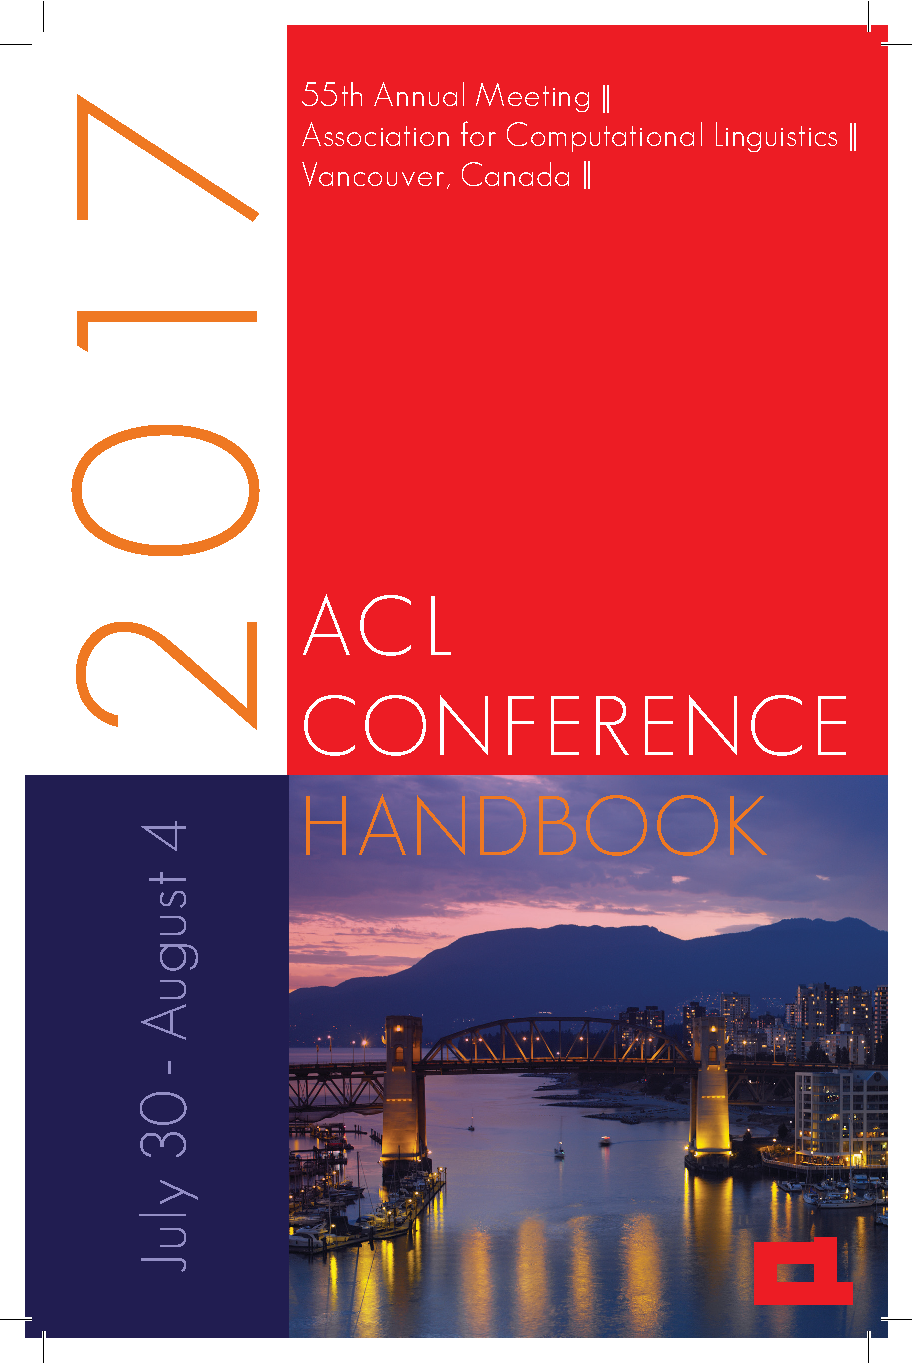
\includepdf[pages={1}]{content/fmatter/cover.jpg}

\thispagestyle{empty}
\vspace*{5.5in}
\noindent
\emph{Cover design by Ying Lin}\\

\noindent
\emph{Cover photo is a derivative of original work by Peyton Stanton available at \url{https://www.flickr.com/photos/peytonstanton/35496401710/}}

\noindent
\emph{\url{https://creativecommons.org/licenses/by-nc/2.0/}}

\noindent

\includegraphics[width=.15in]{content/fmatter/cc.png}
\includegraphics[width=.15in]{content/fmatter/by.png}
\includegraphics[width=.15in]{content/fmatter/nc.png}

\noindent
\emph{Handbook assembled by Jonathan May}\\

\noindent
\emph{Printing by Omnipress of Madison, Wisconsin}

\index{May, Jonathan}
\index{Lin, Ying}
\index{Stanton, Peyton}
\newpage
\cleardoublepage
\fancyfoot[C]{\thepage}
\frontmatter

%% TOC %%%%%%%%%%%%%%%%%%%%%%%%%%%%%%%%%%%%%%%%%%%%%%%%%%%%%%%%%%
\addcontentsline{toc}{chapter}{Table of Contents}
\setcounter{tocdepth}{2}
%\vspace{-2in}
\tableofcontents
\mainmatter
\pagestyle{fancy}

%% PREFACE %%%%%%%%%%%%%%%%%%%%%%%%%%%%%%%%%%%%%%%%%%%%%%%%%%%%%%
\chapter{Conference Information}

\vspace{-4em}

\section{Message from the General Chair}%\vspace{2em}
\setheaders%
    {Message from the General Chair}%
    {Message from the General Chair}
\thispagestyle{emptyheader}


Welcome to New Orleans and to NAACL HLT 2018 – the biggest NAACL to
date.  Natural Language Processing and Computational Linguistics is
constantly growing and changing with a constant flow of new methods
and topics. Every year also sees an even more exciting and diverse
research community, with a steadily increasing number researchers,
companies both large and small, and a vibrant community of
practitioners and students who are excited at the prospect of taking
on the newest challenges of the discipline.  This year’s NAACL HLT
conference reflects what an exciting time this is for our field, and
highlights the vibrancy and vitality of our community.

I feel extremely lucky to be able to work with a fantastic program
committee, especially the two extremely dedicated, creative and
resourceful program chairs: Amanda Stent and Heng Ji. Their
innovations include a new review form, intended to elicit higher
quality reviews, the opportunity for authors to review the reviewers,
the Test-of-Time awards, and a program where poster and demo sessions
run consistently in parallel to the oral sessions, in order to allow
the conference to reflect the ever increasing diversity of research
topics and the corresponding volume of accepted papers.  I am
especially excited about the new Test-of-Time papers award session,
and hope to see this new innovation become a regular part of ACL
conferences.

We have	named the Test-of-Time award in memory of Aravind Joshi, who
left us this year, after having a huge lifetime impact on our
community. We will always remember him for his gentle conversational
style, sharp focus, interest in linguistic, computational and
mathematical properties of language, and his lifetime commitment to
mentoring women in NLP.	I feel extremely lucky to have been one	of his
Ph.D. students.

This year we also introduced an industrial track, with the aim of
featuring papers that focus on scalable, interpretable, reliable and
customer facing methods for industrial applications of Natural
Language Processing. The idea of having such a track was proposed by
Yunyao Li who strongly advocated for it: this proposal was then
discussed and approved by the NAACL board. After that, it was all go,
with an incredible amount of work to promote and organize it by the
industrial track chairs: Jennifer Chu-Carroll, Yunyao Li and Srinivas
Bangalore.

The overall program looks amazing and reflects the cooperative way
that everyone on the committee worked together. What a team! I am so
grateful for getting to be a part of this community of people, and I
really appreciate the enthusiasm and attention to detail reflected in
their hard work: Amanda Stent and Heng Ji (program chairs); Jennifer
Chu-Carroll, Yunyao Li and Srinivas Bangalore (industrial track
chairs); Ying Lin (website chair); Marie Meteer and Jason Williams
(workshop co-chairs); Mohit Bansal and Rebecca Passonneau (tutorial
co-chairs); Yang Liu, Tim Paek, and Manasi Patwardhan (demo
co-chairs); Chris Callison-Burch and Beth Hockey (Family-Friendly
Program Co-Chairs) Stephanie Lukin and Meg Mitchell (publication
co-chairs); Jonathan May (handbook chair); Silvio Ricardo Cordeiro,
Shereen Oraby, Umashanthi Pavalanathan, and Kyeongmin Rim (student
cochairs) along with Swapna Somasundaran and Sam Bowman (Faculty
Advisors) for the student research workshop; Lena Reed (student
volunteer coordinator); Kristy Hollingshead, Kristen Johnson, and
Parisa Kordjamshidi (local sponsorships and exhibits cochairs);
Yonatan Bisk and Wei Xu (publicity and social media chairs); David
Yarowsky and Joel Tetreault (treasurers) and Alexis Palmer and Jason
Baldridge (the NAACL international Sponsorship Team). Also thanks to
Rich at SoftConf for his speedy response to questions and his
willingness to help us innovate with our new review form. And thanks
to Julia Hockenmaier and the whole NAACL Executive Board for always
being willing to consult on any issue.

The program highlights three keynote speakers in the main track: Dilek
Hakkani-T\"{u}r, Kevin Knight, and Charles Yang. We also have two keynote
speakers in the industry track: Mari Ostendorf and Daniel Marcu. These
talks promising to be interesting across a range of issues from
language acquisition in children to the commercial possibilities
of conversational agents. The industry track will also feature
two panels, one on careers in industry (as compared to academia)
and the other on ethics in
NLP. The program also includes six tutorials featuring topics
of current interest and sources of innovation in the field.
We have sixteen workshops
plus the student research workshop: some of these workshops have become
events in themselves with many of them repeated each year.
We will also have plenary sessions for the outstanding paper awards and the
new Test-Of-Time papers award session. 

Any event of this scale can only happen with the the hard work of a
wonderful group of people. I especially want to thank the NAACL board
for being willing to consult on a range of different issues and
Priscilla Rasmussen for taking care of all the millions of details
that need to be looked after every single day to make sure the
logistical aspects of the conference come together.  I want to
especially thank Priscilla for her hard work and creativity organizing
our social event: we first will go to Mardi Gras World to see the
world of wonders created each year for the Mardi Gras. From there we
go to the river, to the dockside River City Plaza and River City
Ballroom for New Orleans' famous cuisine and libations and dancing to
live Zydeco, funk, soul and R\&B.

ACL has been working for several years to increase diversity at our
conferences and in our community. So, taking inspiration from ACL 17,
we aimed to make NAACL family friendly, by providing childcare at the
conference, and encouraging people to bring their families to the
social events and breakfasts. Diversity can also be a consequence of
the support for students to attend the conference that we receive from
the NSF, CRA-CCC and CRA-W: this subsidizes student travel to the student
research workshop as well as their registration and ACL
memberships. When combined with the support we are able to give to our
student volunteers, we aim to make it possible for students from all
over the world to come to the conference and be part of our
community. We also decided, in consultation with the NAACL board, to
provide subsidies to the Widening NLP workshop, which is only being
held for the second time at this year's NAACL (last year called the
Women in NLP workshop).  These subsidies enable participation from
students and young researchers from developing countries to attend the
conference.


I am grateful to our sponsors for their generous contributions, which
add so much to what we can do at the conference. Our Diamond sponsors
are Bloomberg, Google, and TouTiao (ByteDance). The Platinum
sponsor is Amazon. The Gold Sponsors are Ebay, Grammarly, IBM Research, KPMG, Oracle, Poly AI,
Tulane University, Capital One and Two Sigma. The Silver sponsors are Nuance and
Facebook, and the Bronze sponsors are iMerit and USC/ISI.

Finally, there are many more people who through their hard work and
dedication have contributed to make this conference a success: the
area chairs, workshop organizers, tutorial presenters, student
mentors, and reviewers. And of course you all, the attendees without
whom there would be no conference: you are the life and spirit of the
conference and the NAACL community. I hope you all have a
fun and exciting time at NAACL HLT 2018!

\noindent NAACL HLT 2018 General Chair \\
{\it Marilyn Walker}, University of California Santa Cruz \index{Walker, Marilyn}

\clearpage
\section{Message from the Program Committee Co-Chairs}\vspace{2em}
\setheaders%
    {Message from the Program Committee Co-Chairs}%
    {Message from the Program Committee Co-Chairs}
\thispagestyle{emptyheader}
%\renewcommand{\large}{\fontsize{9}{11}\selectfont}
% that's a hack to make this part nicely fill the pages

\setlength{\parskip}{.7ex}
%\setlength{\parindent}{0pt}

\textbf{OLD PLACEHOLDER TEXT FOLLOWS}


Welcome to the 55th Annual Meeting of the Association for
Computational Linguistics! This year, ACL received 751 long paper
submissions and 567 short paper submissions.\footnote{These numbers
  exclude papers that were not reviewed due to formatting, anonymity,
  or double submission violations or that were withdrawn prior to
  review, which was unfortunately a substantial number.} Of the long
papers, 195 were accepted for presentation at ACL — 117 as oral
presentations and 78 as poster presentations (25\% acceptance rate).
107 short papers were accepted — 34 as oral and 73 as poster
presentations (acceptance rate of 18\%). In addition, ACL will also
feature 21 presentations of papers accepted in the  Transactions
  of the Association for Computational Linguistics (TACL). Including
the student research workshop and software demonstrations, the ACL
program swells to a massive total of 367 paper presentations on the
scientific program, representing the largest ACL program to date.

% Min: invited speakers
ACL 2017 will have two distinguished invited speakers: Noah A. Smith
(Associate Professor of Computer Science and Engineering at the
University of Washington) and Mirella Lapata (Professor in the School
of Informatics at the University of Edinburgh).  Both are
well-renowned for their contributions to the field of computational
linguistics and are excellent orators.  We are honored that they have
accepted our invitation to address the membership at this exciting
juncture in our field's history, addressing key issues in
representation learning and multimodal machine translation.

% Min: new innovations
To manage the tremendous growth of our field, we introduced some
changes to the conference. With the rotation of the annual meeting to
the Americas, we anticipated a heavy load of submissions and early on
we decided to have both the long and short paper deadlines merged to
reduce reviewing load and to force authors to take a stand on their
submissions' format.  The joint deadline allowed us to only load our
reviewers once, and also enabled us to have an extended period for
more lengthy dialogue among authors, reviewers and area chairs.  

In addition, oral presentations were shortened to fourteen (twelve)
minutes for long (short) papers, plus time for questions.  While this
places a greater demand on speakers to be concise, we believe it is
worth the effort, allowing far more work to be presented orally. We
also took advantage of the many halls available and expanded the
number of parallel talks to five during most of the conference
sessions.

In keeping with changes introduced in the ACL community from last
year, we continued the practice of recognizing outstanding papers at
ACL. The 22 outstanding papers (15 long, 7 short, 1.6\% of
submissions) represent a broad spectrum of exciting contributions and
have been specially placed on the final day of the main conference
where the program is focused into two parallel sessions of these
outstanding contributions. From these, a best paper and a best short
paper those will be announced in the awards session on Wednesday
afternoon.

%% Following other recent ACL conferences, submissions were reviewed
%% under different categories and using different review forms for
%% empirical/data-driven, theoretical, applications/tools,
%% resources/evaluation, and survey papers. We introduced special fields
%% in the paper submission form for authors to explicitly note the
%% release of open-source implementations to enable reproducibility, and
%% to note freely available datasets.  We also allowed authors to submit
%% appendices of arbitrary length for details that would enable
%% replication; reviewers were not expected to read this material.

%% Another innovation we explored during the review period was the
%% scheduling of short paper review before long paper review. While this
%% was planned to make the entire review period more compact (fitting
%% between the constraints of NAACL 2016 and EMNLP 2016 at either end),
%% we found that reviewing short papers first eliminated many of the
%% surprises for the long paper review process.

%% We sought to follow recently-evolved best practices in planning the
%% poster sessions, so that the many high-quality works presented in that
%% format will be visible and authors and attendees benefit from the
%% interactions during the two poster sessions.

We introduced the chairs'
blog\footnote{\url{https://chairs-blog.acl2017.org/}}, where we strove
to make the selection process of the internal workings of the
scientific committee more transparent.  We have publicly documented
our calls for area chairs, reviewers and accepted papers selection
process.  Via the blog, we communicated several innovations in the
conference organization workflow, of which we would call attention to
two key ones here.

In the review process, we pioneered the use of the Toronto Paper
Matching System, a topic model based approach to the assignment of
reviewers to papers.  We hope this decision will spur other program
chairs to adopt the system, as increased coverage will better the
reviewer/submission matching process, ultimately leading to a higher
quality program.

For posterity, we also introduced the usage of hyperlinks in the
bibliography reference sections of papers, and have worked with the
ACL Anthology to ensure that digital object identifiers (DOIs) appear
in the footer of each paper.  These steps will help broaden the
long-term impact of the work that our community has on the scientific
world at large.


\newpage
There are many individuals we wish to thank for their contributions
to ACL 2017, some multiple times:

\begin{itemize}
\item The 61 area chairs who volunteered for our extra duty. They
  recruited reviewers, led discussions on each paper, replied to
  authors' direct comments to them and carefully assessed each
  submission.  Their input was instrumental in guiding the final
  decisions on papers and selecting the outstanding papers.
%
% Mausam, Omri Abend, Eugene Agichtein, Ron Artstein, Alexandra Balahur,
% Mohit Bansal, Chia-Hui Chang, Grzegorz Chrupała, Mona Diab, Jason
% Eisner, Manaal Faruqui, Raquel Fernandez, Karën Fort, Amir Globerson,
% Hannaneh Hajishirzi, Chiori Hori, Tommi Jaakkola, Yangfeng Ji, Jing
% Jiang, Sarvnaz Karimi, Anna Korhonen, Zornitsa Kozareva, Lun-Wei Ku,
% Nate Kushman, Chia-ying Lee, Oliver Lemon, Roger Levy, Sujian Li,
% Wenjie Li, Kang Liu, Tie-Yan Liu, Yang Liu, Zhiyuan Liu, Minh-Thang
% Luong, Saif M Mohammad, Alexander M Rush, Haitao Mi, Alessandro
% Moschitti, Smaranda Muresan, Preslav Nakov, Graham Neubig, Aurélie
% Névéol, Shimei Pan, Michael Piotrowski, Emily Pitler, Barbara Plank,
% Sujith Ravi, Verena Rieser, Sophie Rosset, Mehroosh Sadrzadeh, Hinrich
% Schütze, Anders Søgaard, Karin Verspoor, Aline Villavicencio, Svitlana
% Volkova, Bonnie Webber, Deyi Xiong, William Yang Wang, Wajdi
% Zaghouani, Yue Zhang and Hai Zhao.

\item Our full program committee of 1,200 hard-working individuals who
  reviewed the conference’s 1,318 submissions (including secondary
  reviewers).
\item TACL editors-in-chief Mark Johnson, Lillian Lee, and Kristina
  Toutanova, for coordinating with us on TACL presentations at ACL.
\item Noah Smith and Katrin Erk, program co-chairs of ACL 2016 and Ani
  Nenkova and Owen Rambow, program co-chairs of NAACL 2016, who we
  consulted several times on short order for help and advice.
\item Wei Lu and Sameer Singh, our well-organized publication chairs,
  with direction and oversight from publication chair mentor Meg
  Mitchell.  Also, Christian Federmann who helped with the local
  handbook.
\item The responsive team at Softconf led by Rich Gerber, who worked
  quickly to resolve problems and who strove to integrate the use of
  the Toronto Paper Matching System (TPMS) for our use.
\item Priscilla Rasmussen and Anoop Sarkar and the local organization
  team, especially webmaster Nitin Madnani.
\item Chris Callison-Burch, our general chair, who kept us
  coordinated with the rest of the ACL 2017 team and helped us free
  our time to concentrate on the key duty of organizing the scientific
  program.
\item Key-Sun Choi, Jing Jiang, Graham Neubig, Emily Pitler, and
  Bonnie Webber who carefully reviewed papers under consideration for
  best paper recognition.
\item Our senior correspondents for the blog, who contributed guest
  posts and advice for writing and reviewing: Waleed Ammar, Yoav
  Artzi, Tim Baldwin, Marco Baroni, Claire Cardie, Xavier Carreras,
  Hal Daumé, Kevin Duh, Chris Dyer, Marti Hearst, Mirella Lapata,
  Emily M. Bender, Aurélien Max, Kathy McKeown, Ray Mooney, Ani
  Nenkova, Joakim Nivre, Philip Resnik, and Joel Tetreault.  Without
  them, the participation of the community through the productive
  comments, and without you the readership, our blog for disseminating
  information about the decision processes would not have been
  possible and a success.
\end{itemize}

We hope that you enjoy ACL 2017 in Vancouver!


\vskip 0.5in
\noindent ACL 2017 program co-chairs\\
Regina Barzilay, Massachusetts Institute of Technology\\
Min-Yen Kan, National University of Singapore


\clearpage
\vspace{2em}

\section{Message from the Industry Track Co-Chairs}\vspace{2em}
\setheaders%
    {Message from the Industry Track Co-Chairs}%
    {Message from the Industry Track Co-Chairs}
\thispagestyle{emptyheader}

\setlength{\parskip}{1ex}

It is our pleasure to welcome you to the inaugural Industry Track in the *ACL family of conferences at NAACL 2018. 

The idea of organizing an industry track stemmed from the challenging issues encountered while attempting to apply state-of-the-art techniques to real-world language problems. As those who have attempted these problems know, practical applications are rarely as well defined as in laboratory settings and the data never as clean. In addition, there may be practical constraints such as computational requirements, processing speed, memory footprint, latency requirements, ease of updating a deployed solution that need to be balanced judiciously, and capability to be embedded as part of a larger system. The NAACL 2018 Industry Track was born out of the desire to provide a forum for researchers, engineers and application developers who are experienced in these issues to exchange ideas, share results and discuss use-cases of successful development and deployments of language technologies in real-world settings. 

Although we thought that the time is ripe in the NLP field for such a forum, and hoped that the community will embrace the opportunity to share their experience with others, it was nonetheless a guessing game as to the amount of interest the track would actually generate. As submissions drew to a close in late February, we were happy to report that we received 91 submissions, far exceeding our expectations (which led to last-minute scrambling to recruit more reviewers, but we're not complaining!). Six of the papers were desk rejects due to non-conformance with submission requirements, and the remaining 85 papers were reviewed by 65 reviewers. We accepted 28 papers -- an acceptance rate of 32.9\% (one paper was subsequently withdrawn after acceptance) of which 19 papers will be presented in oral sessions that run as a parallel track during the main conference, and 8 papers will be presented during poster sessions. Of course, none of this would have been possible without the participation of authors and reviewers, and we would like to convey our heartfelt "thank you" to all the authors for submitting papers and the reviewers for their efforts in the paper selection process.

We analyzed our submissions along a couple of dimensions and would like to share some interesting statistics. First we looked at the submissions with respect to the distribution of author affiliations. As one would expect, the industry track focuses on problems that manifest themselves more readily in industry than in academia. Indeed, of the 85 papers reviewed, 55 papers are authored by researchers/engineers in industry laboratories. The particularly encouraging statistic, however, is that 25 papers are the results of collaboration between those in industry and academia. it would be interesting to track these statistics in future years to see if the collaboration increases as the field continues to mature. The second dimension we analyzed is the geographic distribution of authors by contact author. This being a NAACL conference, it is no surprise that 62\% of the papers came from North America. We are pleased with the participation of authors from other regions, including 22\% from Europe, 14\% from Asia, and 1\% from Africa. 

In addition to paper presentations, we will have two plenary keynote speeches. For the keynote speeches, we aimed to feature researchers who also have first hand experience applying research results to practical applications. To that end, we are honored to have two illustrious members of NLP community --  Daniel Marcu, who co-founded Language Weaver more than 15 years ago and is now the director of MT/NLP at Amazon, and Mari Ostendorf, professor at the University of Washington, who led a team of students to build a social bot that won the 2017 Alexa Prize competition. We are confident that their experiences would be of immense interest to the larger NLP community.

Another highlight of the industry track includes two panel discussions on topics of increasing importance in the community. The first panel, ``Careers in Industry,'' moderated by Philip Resnik, professor at University of Maryland, is primarily geared toward students and recent graduates who are exploring careers in industry versus academia. The panel will feature experienced professionals who have worked in both environments to share their experience and offer advice, based on questions gathered from the *ACL community earlier this year. The second panel, ``Ethics in NLP,'' will be moderated by Dirk Hovy, professor at Università Bocconi, and will focus on raising awareness of the emerging issues of biases present in NLP/AI solutions, the social implications of such biases, and what we, as NLP practitioners, can do to reduce them. 

With the overwhelming response to the call for papers, the language community has unambiguously endorsed the relevance of the Industry track in the milieu of annual conferences.  As organizers, we have attempted to amplify this endorsement by bringing to the participants an invigorating technical program. We hope through your engaging discussions and active participation during the sessions, you will unanimously support and nurture the concept of an Industry track in NLP conferences over the years to come.



\vskip 0.5in
\noindent Srinivas Bangalore (Interactions Labs) \\
Jennifer Chu-Carroll (Elemental Cognition) \\
Yunyao Li (IBM Research - Almaden) \\
NAACL 2018 Industry Track Co-Chairs

\index{Bangalore, Srinivas}
\index{Chu-Carroll, Jennifer}
\index{Li, Yunyao}




\clearpage
\setheaders{}{}
\markboth{}{} % clear the right header
\markright{}{} % clear the right header

\section{Organizing Committee}{}\vspace{2em}

\setlength{\parindent}{0pt}

{\bf General Chair} \\
Marilyn Walker, University of California, Santa Cruz

{\bf Program Co-chairs} \\
Heng Ji, Rensselaer Polytechnic Institute\\
Amanda Stent, Bloomberg

{\bf Local Arrangements Chair} \\
Priscilla Rasmussen, ACL\\

{\bf Workshop Co-chairs} \\
Marie Meteer, Brandeis University\\
Jason Williams, Microsoft Research

{\bf Industry Track Co-chairs} \\
Srinivas Bangalore, Interactions \\
Jennifer Chu-Carroll, Elemental Cognition \\
Yunyao Li, IBM

{\bf Tutorial Co-chairs} \\
Mohit Bansal, University of North Carolina\\
Rebecca Passonneau, Pennsylvania State University

{\bf Publication Co-chairs} \\
Stephanie Lukin, U.S. Army Research Laboratory, Santa Monica\\
Margaret Mitchell, Google

{\bf Demonstration Co-chairs} \\
Yang Liu, University of Texas at Dallas\\
Tim Paek, Apple\\
Manasi Patwardhan, Tata Consultancy Services Research, India

{\bf Family-Friendly Program Co-Chairs} \\
Chris Callison-Burch, University of Pennsylvania\\
Beth Hockey, Intel

{\bf Student Research Workshop Organizers} \\
Silvio Ricardo Cordeiro, Federal University of Rio Grande do Sul \\
Shereen Oraby, University of California, Santa Cruz \\
Umashanthi Pavalanathan, Georgia Institute of Technology\\
Kyeongmin Rim, Brandeis University \\

{\bf Faculty Advisors to the Student Research Workshop} \\
Swapna Somasundaran, ETS Princeton\\
Sam Bowman, New York University

{\bf Publicity and Social Media Chairs} \\
Yonatan Bisk, University of Washington \\
Wei Xu, Ohio State University

{\bf Conference Handbook Chair} \\
Jonathan May, University of Southern California Information Sciences Institute

{\bf Student Volunteer Coordinator} \\
Lena Reed, University of California, Santa Cruz


{\bf Website Chair} \\
Ying Lin, Rensselaer Polytechnic Institute


%%%%%%%%%%%%%%%%%%%%%%%%%%%%%%%%%%%%%%%%%%%%%%%%%%%%%%%%%%%%%%%%%%%%%%%%

\clearpage
\section{Program Committee}
\setlength{\parindent}{0pt}

\vspace*{0.5cm}

{\bf Program Co-chairs} \\
Heng Ji, Rensselaer Polytechnic Institute\\
Amanda Stent, Bloomberg

{\bf Area Chairs} \\
                \emph{Cognitive Modeling/Psycholinguistics} \\
                                    \hspace*{0.2in} Morteza Dehghani, University of Southern California \\
                                    \hspace*{0.2in} Kristy Hollingshead Seitz, Institute for Human \& Machine Cognition \\
                            \emph{Dialogue and Interactive Systems:} \\
                                    \hspace*{0.2in} Yun-Nung (Vivian) Chen, National Taiwan University \\
                                    \hspace*{0.2in} Gabriel Skantze, KTH Royal Institute of Technology \\
                            \emph{Discourse and Pragmatics} \\
                                    \hspace*{0.2in} Jacob Eisenstein, Georgia Institute of Technology \\
                                    \hspace*{0.2in} Junyi (Jessy) Li, University of Texas at Austin \\
                                    \hspace*{0.2in} Annie Louis, University of Edinburgh \\
                                    \hspace*{0.2in} Yi Yang, Bloomberg LP \\
                            \emph{Generation} \\
                                    \hspace*{0.2in} Dimitra Gkatzia, Edinburgh Napier University \\
                                    \hspace*{0.2in} Shashi Narayan, University of Edinburgh \\
                                    \hspace*{0.2in} Michael White, Ohio State University \\
                            \emph{Information Extraction} \\
                                    \hspace*{0.2in} Mausam, Indian Institute of Technology Delhi \\
                                    \hspace*{0.2in} Dan Bikel, Google \\
                                    \hspace*{0.2in} Chia-Hui Chang, National Central University \\
                                    \hspace*{0.2in} Bonan Min, BBN \\
                                    \hspace*{0.2in} Aur\'{e}lie N\'{e}v\'{e}ol, CNRS \\
                                    \hspace*{0.2in} Marius Pasca, Google \\
                                    \hspace*{0.2in} Hinrich Sch\"{u}tze, Ludwig Maximilian University of Munich \\
                                    \hspace*{0.2in} Avirup Sil, IBM Research AI \\
                                    \hspace*{0.2in} Michael Strube, HITS gGmbH \\
                            \emph{Machine Learning for NLP} \\
                                    \hspace*{0.2in} Chris Dyer, Google DeepMind \\
                                    \hspace*{0.2in} Ozan Irsoy, Cornell University \\
                                    \hspace*{0.2in} Tie-Yan Liu, Microsoft Research \\
                                    \hspace*{0.2in} Raymond Mooney, University of Texas at Austin  \\
                            \emph{Machine Translation} \\
                                    \hspace*{0.2in} Marine Carpuat, University of Maryland \\
                                    \hspace*{0.2in} Kyunghyun Cho, New York University \\
                                    \hspace*{0.2in} Daniel Marcu, Amazon \\
                                    \hspace*{0.2in} Taro Watanabe, Google \\
                                    \hspace*{0.2in} Deyi Xiong, Soochow University \\
                            \emph{NLP Applications} \\
                                    \hspace*{0.2in} Jinho Choi,  \\
                                    \hspace*{0.2in} Joel Tetreault, Grammarly \\
                            \emph{Phonology, Morphology and Word Segmentation} \\
                                    \hspace*{0.2in} Jennifer Foster, Dublin City University \\
                                    \hspace*{0.2in} Barbara Plank, University of Groningen \\
                            \emph{Question Answering} \\
                                    \hspace*{0.2in} Eugene Agichtein, Emory University \\
                                    \hspace*{0.2in} Hannaneh Hajishirzi, University of Washington \\
                                    \hspace*{0.2in} Idan Szpektor, Google \\
                            \emph{Semantics} \\
                                    \hspace*{0.2in} Yoav Artzi, Cornell University \\
                                    \hspace*{0.2in} Mona Diab, George Washington University \\
                                    \hspace*{0.2in} Kevin Duh, Johns Hopkins University \\
                                    \hspace*{0.2in} Jonathan May, University of Southern California \\
                                    \hspace*{0.2in} Preslav Nakov, Qatar Computing Research Institute \\
                                    \hspace*{0.2in} Roi Reichart, Technion - Israel Institute of Technology \\
                                    \hspace*{0.2in} Dan Roth, University of Pennsylvania \\
                                    \hspace*{0.2in} Scott Wen-tau Yih, Allen Institute for Artificial Intelligence \\
                            \emph{Sentiment Analysis} \\
                                    \hspace*{0.2in} Smaranda Muresan, Columbia University \\
                                    \hspace*{0.2in} Swapna Somasundaran, ETS Princeton \\
                            \emph{Social Media Analysis and Computational Social Science} \\
                                    \hspace*{0.2in} Mark Dredze, Johns Hopkins University \\
                                    \hspace*{0.2in} Miles Osborne, Bloomberg \\
                                    \hspace*{0.2in} Alan Ritter, Ohio State University \\
                                    \hspace*{0.2in} Sara Rosenthal, IBM \\
                                    \hspace*{0.2in} William Yang Wang, University of California, Santa Barbara \\
                            \emph{Speech} \\
                                    \hspace*{0.2in} Eric Fosler-Lussier, Ohio State University \\
                                    \hspace*{0.2in} Dilek Hakkani-Tur, Google \\
                                    \hspace*{0.2in} Mari Ostendorf, University of Washington \\
                            \emph{Summarization} \\
                                    \hspace*{0.2in} George Giannakopoulos, NCSR "Demokritos" \\
                                    \hspace*{0.2in} Xiaojun Wan, Peking University \\
                                    \hspace*{0.2in} Lu Wang, Northeastern University \\
                            \emph{Tagging, Chunking, Syntax and Parsing} \\
                                    \hspace*{0.2in} Michael Collins, Columbia University \\
                                    \hspace*{0.2in} Yoav Goldberg, Bar Ilan University \\
                                    \hspace*{0.2in} Daisuke Kawahara, Kyoto University \\
                                    \hspace*{0.2in} Emily Pitler, Google \\
                                    \hspace*{0.2in} Anders S{\o}gaard, University of Copenhagen \\
                                    \hspace*{0.2in} Aline Villavicencio, University of Essex (UK) and Federal University of Rio Grande do Sul (Brazil) \\
                            \emph{Text Mining} \\
                                    \hspace*{0.2in} Kai-wei Chang, University of Virginia \\
                                    \hspace*{0.2in} Jing Jiang, Singapore Management University \\
                                    \hspace*{0.2in} Zornitsa Kozareva, Google \\
                                    \hspace*{0.2in} Chin-Yew Lin, Microsoft Research Asia \\
                            \emph{Theory and Formalisms} \\
                                    \hspace*{0.2in} David Chiang, University of Notre Dame \\
                                    \hspace*{0.2in} Daniel Gildea, University of Rochester \\
                                    \hspace*{0.2in} Giorgio Satta, University of Padua \\
                            \emph{Vision, Robotics and Other Grounding} \\
                                    \hspace*{0.2in} Joyce Chai, Michigan State University \\
                                    \hspace*{0.2in} Vicente Ordonez, University of Virginia \\


\clearpage
\setheaders{}{}
\setheaders{}{}
\section{Outstanding Reviewers}{}

We thank all reviewers for spending their valuable time on reviewing NAACL paper submissions! The following are outstanding reviewers nominated by area chairs:

\begin{multicols}{3}
  \begin{itemize}\raggedright
    \setlength\itemsep{0em}
\reviewer{Omri}{Abend}
\reviewer{Manex}{Agirrezabal}
\reviewer{Cem}{Akkaya}
\reviewer{Enrique}{Alfonseca}
\reviewer{Dimitrios}{Alikaniotis}
\reviewer{Tim}{Anderson}
\reviewer{Layla}{El Asri}
\reviewer{Michael}{Auli}
\reviewer{Wilker}{Aziz}
\reviewer{Mohit}{Bansal}
\reviewer{Valerio}{Basile}
\reviewer{Roberto}{Basili}
\reviewer{Beata}{Beigman Klebanov}
\reviewer{Jonathan}{Berant}
\reviewer{Delphine}{Bernhard}
\reviewer{Rahul}{Bhagat}
\reviewer{Bernd}{Bohnet}
\reviewer{Chris}{Brew}
\reviewer{Aoife}{Cahill}
\reviewer{Ruket}{Cakici}
\reviewer{Yuan}{Cao}
\reviewer{Giusepe}{Carenini}
\reviewer{Asli}{Celikyilmaz}
\reviewer{Cheng}{Chen}
\reviewer{Shamil}{Chollampatt}
\reviewer{Paul}{Crook}
\reviewer{Xiaodong}{Cui}
\reviewer{Giovanni}{da San Martino}
\reviewer{Andrew}{Dai}
\reviewer{Kees}{van Deemter}
\reviewer{Rodolfo}{Delmonte}
\reviewer{Gerard}{de Melo}
\reviewer{Dina}{Demner­-Fushman}
\reviewer{Lingjia}{Deng}
\reviewer{Mark}{Dras}
\reviewer{Ondřej}{Dušek}
\reviewer{Marc}{Dymetman}
\reviewer{Steffen}{Eger}
\reviewer{Markus}{Egg}
\reviewer{Keelan}{Evanini}
\reviewer{Olivier}{Ferret}
\reviewer{Katja}{Filippova}
\reviewer{Michael}{Flor}
\reviewer{Anette}{Frank}
\reviewer{Michel}{Galley}
\reviewer{Claire}{Gardent}
\reviewer{Kallirroi}{Georgila}
\reviewer{Yvette}{Graham}
\reviewer{Debanjan}{Ghosh}
\reviewer{Francisco}{Guzman}
\reviewer{Thierry}{Hamon}
\reviewer{Helen}{Hastie}
\reviewer{Michael}{Heilman}
\reviewer{James}{Hendler}
\reviewer{Derrick}{Higgins}
\reviewer{Chiori}{Hori}
\reviewer{Veronique}{Hoste}
\reviewer{Julian}{Hough}
\reviewer{Hen-Hsen}{Huang}
\reviewer{Rebecca}{Hwa}
\reviewer{Marcin}{Junczys-Dowmunt}
\reviewer{Rasoul}{Kaljahi}
\reviewer{Lauri}{Karttunen}
\reviewer{David}{Kauchak}
\reviewer{Anna}{Kazantseva}
\reviewer{Andrew}{Kehler}
\reviewer{Kian}{Kenyon-Dean}
\reviewer{Alistair}{Knott}
\reviewer{Hayato}{Kobayashi}
\reviewer{Mamoru}{Komachi}
\reviewer{Alexander}{Koller}
\reviewer{Patrik}{Lambert}
\reviewer{Mirella}{Lapata}
\reviewer{John}{Lee}
\reviewer{Yves}{Lepage}
\reviewer{James}{Lester}
\reviewer{Omer}{Levy}
\reviewer{Yanran}{Li}
\reviewer{Chu-Cheng}{Lin}
\reviewer{Elena}{Lloret}
\reviewer{Karen}{Livescu}
\reviewer{Bing}{Liu}
\reviewer{Stephanie}{Lukin}
\reviewer{Nitin}{Madnani}
\reviewer{Adam}{Makarucha}
\reviewer{Yoichi}{Matsuyama}
\reviewer{Karen}{Mazidi}
\reviewer{Diana}{McCarthy}
\reviewer{Philipp}{Meerkamp}
\reviewer{Oren}{Melamud}
\reviewer{Emiel}{Van Miltenburg}
\reviewer{Saif}{Mohammad}
\reviewer{Taesun}{Moon}
\reviewer{Nasrin}{Mostafazadeh}
\reviewer{Philippe}{Muller}
\reviewer{Karthik}{Narasimhan}
\reviewer{Dong}{Nguyen}
\reviewer{Garett}{Nicolai}
\reviewer{Hugo Gonçalo}{Oliveira}
\reviewer{Lilja}{Øvrelid}
\reviewer{Alexis}{Palmer}
\reviewer{Laura}{Perez-Beltrachini}
\reviewer{Paul}{Piwek}
\reviewer{Thierry}{Poibeau}
\reviewer{Fred}{Popowich}
\reviewer{Daniel}{Preoţiuc-Pietro}
\reviewer{Carlos}{Ramisch}
\reviewer{Sujith}{Ravi}
\reviewer{Paul}{Rayson}
\reviewer{Sravana}{Reddy}
\reviewer{Marek}{Rei}
\reviewer{Ehud}{Reiter}
\reviewer{Ludovic}{Rheault}
\reviewer{Giuseppe}{Riccardi}
\reviewer{Mark}{Riedl}
\reviewer{Laura}{Rimel}
\reviewer{Brian}{Roark}
\reviewer{Marcus}{Rohrbach}
\reviewer{Melissa}{Roemmele}
\reviewer{Eric}{Rosen}
\reviewer{Johann}{Roturier}
\reviewer{Markus}{Saers}
\reviewer{Allen}{Schmaltz}
\reviewer{Jodi}{Schneider}
\reviewer{H. Andrew}{Schwartz}
\reviewer{Roy}{Schwartz}
\reviewer{Donia}{Scott}
\reviewer{Advaith}{Siddharthan}
\reviewer{Michel}{Simard}
\reviewer{Kairit}{Sirts}
\reviewer{Jose}{de Souza}
\reviewer{Somayajulu}{Sripada}
\reviewer{Matthew}{Stone}
\reviewer{Kristina}{Striegnitz}
\reviewer{John}{Sylak-Glassman}
\reviewer{Kapil}{Thadani}
\reviewer{Mariët}{Theune}
\reviewer{Timothy}{Baldwin}
\reviewer{Antonio}{Toral}
\reviewer{Marco}{Turchi}
\reviewer{Andreas}{Vlachos}
\reviewer{Leo}{Wanner}
\reviewer{Michael}{Wiegand}
\reviewer{Shuly}{Winter}
\reviewer{Sam}{Wiseman}
\reviewer{Jiajun}{Zhang}
\reviewer{Arkaitz}{Zubiaga}
\end{itemize}
\end{multicols}


\section{Ad-hoc Reviewers}

The following are our heroes and heroines! They volunteered their time when we were painfully chasing late reviews. 

\begin{multicols}{3}
  \begin{itemize}\raggedright
    \setlength\itemsep{0em}
\reviewer{Cem}{Akkaya}
\reviewer{Héctor}{Martínez Alonso}
\reviewer{Waleed}{Ammar}
\reviewer{Gabor}{Angeli}
\reviewer{Reihane}{Boghrati}
\reviewer{Iacer}{Calixto}
\reviewer{Leonardo}{Campillos}
\reviewer{Kai}{Cao}
\reviewer{Özlem}{Çetinoğlu}
\reviewer{Yee Seng}{Chan}
\reviewer{Michael}{Collins}
\reviewer{Çağrı}{Çöltekin}
\reviewer{Silvio Ricardo}{Cordeiro}
\reviewer{Bo}{Dai}
\reviewer{Noura}{Farra}
\reviewer{Michael}{Flor}
\reviewer{Radu}{Florian}
\reviewer{Justin}{Garten}
\reviewer{Tao}{Ge}
\reviewer{Debanjan}{Ghosh}
\reviewer{Jiatao}{Gu}
\reviewer{Keith}{Hall}
\reviewer{Benjamin}{Heinzerling}
\reviewer{Xianpei}{Han}
\reviewer{Rasoul}{Kaljahi}
\reviewer{Philipp}{Koehn}
\reviewer{Jonathan K.}{Kummerfeld}
\reviewer{Xiang}{Li}
\reviewer{Elena}{Lloret}
\reviewer{Bing}{Liu}
\reviewer{Jose David}{Lopes}
\reviewer{Di}{Lu}
\reviewer{Nikolaos}{Malandrakis}
\reviewer{Jeff}{Mitchell}
\reviewer{Saif}{Mohammad}
\reviewer{Matthew}{Mulholand}
\reviewer{Vivi}{Nastase}
\reviewer{Dong}{Nguyen}
\reviewer{Thienn Huu}{Nguyen}
\reviewer{Hugo Gonçalo}{Oliveira}
\reviewer{Shereen}{Oraby}
\reviewer{Vinodkumar}{Prabhakaran}
\reviewer{Sujith}{Ravi}
\reviewer{Sophie}{Rosset}
\reviewer{Natalie}{Schluter}
\reviewer{Roy}{Schwartz}
\reviewer{Lanbo}{She}
\reviewer{Amanda}{Stent}
\reviewer{Veselin}{Stoyanov}
\reviewer{Keh-Yih}{Su}
\reviewer{Chen-Tse}{Tsai}
\reviewer{Gokhan}{Tur}
\reviewer{Svitlana}{Volkova}
\reviewer{Joachim}{Wagner}
\reviewer{Chi}{Wang}
\reviewer{Taro}{Watanabe}
\reviewer{Chris}{Waterson}
\reviewer{Rodrigo}{Wilkens}
\reviewer{Mark}{Yatskar}
\reviewer{Wenpeng}{Yin}
\reviewer{Boliang}{Zhang}
\reviewer{Arkaitz}{Zubiaga}
\end{itemize}
\end{multicols}

\clearpage
\setheaders{}{}
\setheaders{}{}
\section{Meal Info}{}

The following meals are provided as part of your registration fee:

\begin{itemize}
\item A full buffet breakfast will be provided each day from 07:30--09:00 in the \BreakLoc
\item Mid-morning breaks include coffee and tea in the \BreakLoc
\item Mid-afternoon breaks include coffee, tea, soda, water, and snacks in the \BreakLoc
\item The Welcome Reception on Friday, June 1st, from 18:00--21:00, will include a light dinner
\item The Recruitment Lunch on Saturday, June 2nd, 12:30--14:00, is intended for students and recruiters and will include a light lunch
\item A full dinner buffet is provided during the Social Event on Sunday, June 3rd 
\end{itemize}

\clearpage

%% TUTORIALS %%%%%%%%%%%%%%%%%%%%%%%%%%%%%%%%%%%%%%%%%%%%%%%%%%%%
\setdaydateyear{Friday}{June 1}{2018}
% This file is just done manually

\chapter{Workshops and Tutorials: \daydate}
\thispagestyle{emptyheader}
\setheaders{Tutorials}{\daydateyear}
\setlength{\parindent}{0in}
\setlength{\parskip}{2ex}
\renewcommand{\baselinestretch}{0.87}

\newcommand{\tutorialmorningtime}{09:00--12:30}
\newcommand{\tutorialafternoontime}{14:00--17:30}
% JM: normally shouldn't be here, added to deal with an annoying line break
% in 2018
\newcommand{\tutol}{\hspace{-.25in}}
\section*{Overview}
\renewcommand{\arraystretch}{1.2}
\begin{SingleTrackSchedule}
  07:30 & -- & 18:00 &
  {\bfseries Registration} \hfill\emph{\RegistrationLoc}\\
  \\[-2mm]
  07:30 & -- & 9:00 &
  {\bfseries Breakfast} \hfill\emph{\BreakfastLoc}\\
  \\[-2mm]
  08:30 & -- & 18:00 &
  {\bfseries WiNLP: Widening NLP} \hfill\emph{\WShopLocWiNLP}\\
  \\[-2mm]
  09:00 & -- & 12:30 &
  {\bfseries Morning Tutorials} \hfill\\
  \\[-2mm]
  & & & \tutol\papertitle{naacl2018-tutorials-014}\hfill\emph{\TutLocA}\newline
  \tutol\tutorialauthors{naacl2018-tutorials-014} \\
  \\[-2mm]
  & & & \tutol\papertitle{naacl2018-tutorials-034}\hfill\emph{\TutLocB}\newline
  \tutol\tutorialauthors{naacl2018-tutorials-034} \\
  \\[-2mm]
  & & & \tutol\papertitle{naacl2018-tutorials-048}\hfill\emph{\TutLocC}\newline
  \tutol\tutorialauthors{naacl2018-tutorials-048} \\
  \\[-2mm]
  10:00 & -- & 10:30 &
  {\bfseries Coffee break}\\
  \\[-2mm]
  12:30 & -- & 14:00 &
  {\bfseries Lunch break}\\
  \\[-2mm]
  14:00 & -- & 17:30 &
  {\bfseries Afternoon Tutorials} \hfill\\
  \\[-2mm]
  & & & \tutol\papertitle{naacl2018-tutorials-008}\hfill\emph{\TutLocD}\newline
  \tutol\tutorialauthors{naacl2018-tutorials-008} \\
  \\[-2mm]
  & & & \tutol\papertitle{naacl2018-tutorials-043}\newline
  \tutol\tutorialauthors{naacl2018-tutorials-043}\hfill\emph{\TutLocE} \\
  \\[-2mm]
  & & & \tutol\papertitle{naacl2018-tutorials-033}\hfill\emph{\TutLocF}\newline
  \tutol\tutorialauthors{naacl2018-tutorials-033} \\
  \\[-2mm]
  15:00 & -- & 15:30 &
  {\bfseries Coffee break}\\
  \\[-2mm]
  18:00 & -- & 21:00 &
  {\bfseries Welcome Reception} \hfill \emph{\WelcomeReceptionLoc}\\
  \\[-2mm]
\end{SingleTrackSchedule}
\setheaders{One-day Workshops}{\daydateyear}
\begin{wsschedule}
  {WiNLP: Widening NLP}
  {4}{WShopWiNLP}
  {WiNLP:1}
  {\WShopLocWiNLP}
  
\item[] {\Large\bfseries Friday, June 1, 2018}\\\vspace{1.5ex}

\vspace{1ex}
\item[] {\bfseries Session I: Opening, Invited Talk I, and Oral Presentations}

\vspace{1ex}
\item[07:30--18:00] {\bfseries  NAACL Registration}

\vspace{1ex}
\item[08:30--09:00] {\bfseries  Opening Remarks: Libby Barak, Amittai Axelrod, Diyi Yang, Lucie Flekova, Zeerak Waseem}

\vspace{1ex}
\item[08:55--09:30] {\bfseries  Invited Talk I: Su Jian - Semantic and Sentiment Analysis for Knowledge Base Population} \index{Jian, Su}

\vspace{1ex}
\item[09:30--10:30] {\bfseries  Oral Presentations}
\item[09:30--09:50] \wspaperentry{winlp18-081}
\item[09:50--10:10] \wspaperentry{winlp18-026}
\item[10:10--10:30] \wspaperentry{winlp18-041}

\vspace{1ex}
\item[10:30--11:00] {\bfseries  Coffee Break}

\vspace{1ex}
\item[] {\bfseries Session II: Invited Talk, Mentoring}

\vspace{1ex}
\item[11:00--11:35] {\bfseries  Invited Talk II: Natalie Schluter - The glass ceiling in NLP} \index{Schluter, Natalie}

\vspace{1ex}
\item[11:35--12:00] {\bfseries  Mentoring}

\vspace{1ex}
\item[12:00--13:00] {\bfseries  Lunch}

\vspace{1ex}
\item[] {\bfseries Session III: Poster Presentations, Career Panel}

\vspace{1ex}
\item[13:00--14:30] {\bfseries  Poster Presentations}
\item[13:00--14:30] \wspaperentry{winlp18-002}
\item[13:00--14:30] \wspaperentry{winlp18-003}
\item[13:00--14:30] \wspaperentry{winlp18-005}
\item[13:00--14:30] \wspaperentry{winlp18-007}
\item[13:00--14:30] \wspaperentry{winlp18-008}
\item[13:00--14:30] \wspaperentry{winlp18-009}
\item[13:00--14:30] \wspaperentry{winlp18-010}
\item[13:00--14:30] \wspaperentry{winlp18-011}
\item[13:00--14:30] \wspaperentry{winlp18-012}
\item[13:00--14:30] \wspaperentry{winlp18-013}
\item[13:00--14:30] \wspaperentry{winlp18-014}
\item[13:00--14:30] \wspaperentry{winlp18-015}
\item[13:00--14:30] \wspaperentry{winlp18-017}
\item[13:00--14:30] \wspaperentry{winlp18-018}
\item[13:00--14:30] \wspaperentry{winlp18-019}
\item[13:00--14:30] \wspaperentry{winlp18-021}
\item[13:00--14:30] \wspaperentry{winlp18-023}
\item[13:00--14:30] \wspaperentry{winlp18-024}
\item[13:00--14:30] \wspaperentry{winlp18-025}
\item[13:00--14:30] \wspaperentry{winlp18-027}
\item[13:00--14:30] \wspaperentry{winlp18-028}
\item[13:00--14:30] \wspaperentry{winlp18-029}
\item[13:00--14:30] \wspaperentry{winlp18-030}
\item[13:00--14:30] \wspaperentry{winlp18-033}
\item[13:00--14:30] \wspaperentry{winlp18-034}
\item[13:00--14:30] \wspaperentry{winlp18-035}
\item[13:00--14:30] \wspaperentry{winlp18-049}
\item[13:00--14:30] \wspaperentry{winlp18-053}
\item[13:00--14:30] \wspaperentry{winlp18-054}
\item[13:00--14:30] \wspaperentry{winlp18-055}
\item[13:00--14:30] \wspaperentry{winlp18-056}
\item[13:00--14:30] \wspaperentry{winlp18-057}
\item[13:00--14:30] \wspaperentry{winlp18-059}
\item[13:00--14:30] \wspaperentry{winlp18-061}
\item[13:00--14:30] \wspaperentry{winlp18-062}
\item[13:00--14:30] \wspaperentry{winlp18-063}
\item[13:00--14:30] \wspaperentry{winlp18-064}
\item[13:00--14:30] \wspaperentry{winlp18-070}
\item[13:00--14:30] \wspaperentry{winlp18-072}
\item[13:00--14:30] \wspaperentry{winlp18-073}
\item[13:00--14:30] \wspaperentry{winlp18-074}
\item[13:00--14:30] \wspaperentry{winlp18-075}
\item[13:00--14:30] \wspaperentry{winlp18-076}
\item[13:00--14:30] \wspaperentry{winlp18-077}
\item[13:00--14:30] \wspaperentry{winlp18-078}
\item[13:00--14:30] \wspaperentry{winlp18-079}
\item[13:00--14:30] \wspaperentry{winlp18-080}
\item[13:00--14:30] \wspaperentry{winlp18-082}

\vspace{1ex}
\item[14:30--15:30] {\bfseries  Career Panel: Houda Bouamor, Barbara Plank, Mugizi Robert Rwebangira, and Amanda Stent} \index{Bouamor, Houda} \index{Plank, Barbara} \index{Rwebangira, Mugizi} \index{Stent, Amanda}

\vspace{1ex}
\item[15:30--15:55] {\bfseries  Coffee Break}

\vspace{1ex}
\item[] {\bfseries Session IV: Invited Talk, Oral Presentations, Closing, Mentor Meetup}

\vspace{1ex}
\item[15:55--16:30] {\bfseries  Invited Talk III: Claire Cardie - ``Information Extraction: What Goes Around Comes Around''} \index{Cardie, Claire}

\vspace{1ex}
\item[16:30--17:10] {\bfseries  Oral Presentations}
\item[16:30--16:50] \wspaperentry{winlp18-004}
\item[16:50--17:10] \wspaperentry{winlp18-042}

\vspace{1ex}
\item[17:10--17:30] {\bfseries  Closing Remarks - Libby Barak, Amittai Axelrod, Diyi Yang, Lucie Flekova, Zeerak Waseem}

\vspace{1ex}
\item[17:30--18:00] {\bfseries  One-on-One Mentor Meetup}

\vspace{1ex}
\item[18:30] {\bfseries  NAACL Welcome Reception}

\end{wsschedule}
\clearpage
\setheaders{Tutorials}{\daydateyear}
\clearpage\section{Message from the Tutorial Co-Chairs}\vspace{2em}
\setheaders%
    {Message from the Tutorial Co-Chairs}%
    {Message from the Tutorial Co-Chairs}
\thispagestyle{emptyheader}

\setlength{\parskip}{1ex}

This section contains the abstracts of the ACL 2017 tutorials. This year we had a joint call-for-tutorials, coordinated with the EACL and EMNLP co-chairs (6 co-chairs in total). We received 26 submissions for the joint ACL/EACL/EMNLP call, and it was a difficult task to make a final selection. The six co-chairs applied the following criteria for evaluation: relevance to ACL community, quality of proposal, quality of instructor, estimate of attendance, relevance of area. The tutorials were then assigned to venues trying to respect proposers' preferences and to balance topics across venues. Nine tutorials had ACL as the preferred conference, from which one was rejected, two were redirected to EMNLP and the rest (six of them) was accepted. All six are organised as half-day tutorials.

We are very grateful to Alex Klementiev and Lucia Specia (EACL tutorial chairs), Nathan Schneider and Alexandra Birch (EMNLP tutorial chairs), Priscilla Rasmussen and Anoop Sarkar (local chairs), Wei Lu, Sameer Singh and Margaret Mitchell (publication chairs), Min-Yen Kan and Regina Barzilay (program co-chairs) and of course Chris Callison-Burch (general chair) for various kinds of help, advice and assistance offered during the process of putting the tutorial programme and materials together. Most importantly, we would like to thank the tutorial presenters for the time and effort in preparing and presenting the tutorials.

We hope you will enjoy the tutorials!

\vskip 0.5in
\noindent
ACL 2017 Tutorial Chairs\\
\noindent
Maja Popović, Humboldt-Universität zu Berlin\\
\noindent
Jordan Boyd-Graber, University of Colorado, Boulder\\

\index{Popović, Maja}
\index{Boyd-Graber, Jordan}

\setheaders{Tutorials}{\daydateyear}
\clearpage\begin{tutorial}
  {Natural Language Processing for Precision Medicine}
  {tutorial-001}
  {\daydateyear, \tutorialmorningtime}
  {\TutLocA}
\end{tutorial}

We will introduce precision medicine and showcase the vast opportunities for NLP in this burgeoning field with great societal impact. We will review pressing NLP problems, state-of-the art methods, and important applications, as well as datasets, medical resources, and practical issues. The tutorial will provide an accessible overview of biomedicine, and does not presume knowledge in biology or healthcare. The ultimate goal is to reduce the entry barrier for NLP researchers to contribute to this exciting domain.

\vspace{2ex}\centerline{\rule{.5\linewidth}{.5pt}}\vspace{2ex}
\setlength{\parskip}{1ex}\setlength{\parindent}{0ex}

  {\bfseries Hoifung Poon} is a Researcher at Microsoft Research Redmond. His research interests lie in advancing machine learning and natural language processing (NLP) to help automate discovery and decision support in precision medicine. He received his Ph.D. in computer science \& engineering at the University of Washington. His past work has been recognized with Best Paper Awards from premier NLP and machine learning venues such as NAACL-09 (unsupervised morphological segmentation), EMNLP-09 (unsupervised semantic parsing), and UAI-11 (sum-product networks).
  \index{Poon, Hoifung}

  {\bfseries Chris Quirk} is a Principal Researcher at Microsoft Research Redmond. Since joining Microsoft Research in 2001, his research has focused on effective computational systems for aiding human communication, understanding, and task completion. His primary focus is in machine translation, building practical and widely-used system implementations and authoring a number of influential papers. He has also worked in paraphrase, information extraction, and most recently biological applications of natural language processing and machine learning. He has served on numerous program committees, acted Area Chair (ACL 2010, EMNLP 2012), and is currently an action editor of the TACL journal.
  \index{Quirk, Chris}

  {\bfseries Kristina Toutanova} is a Staff Research Scientist at Google Research Seattle and affiliate faculty member at the University of Washington. In 2005, she obtained her Ph.D. from the Computer Science Department at Stanford University, where she was advised by Christopher Manning. She focuses on modeling the structure of natural language using machine learning, in the areas of semantic parsing, knowledge extraction, information retrieval, and text-to-text generation. She has coauthored more than 50 publications at refereed conferences and journals, including four papers that have won awards at conferences (EMNLP, NAACL, CoNLL, ECML). She served as a program co-chair for CoNLL 2008 and ACL 2014 and is currently serving as a co-editor-in-chief of the TACL journal.
  \index{Toutanova, Kristina}

  {\bfseries Wen-tau Yih} is a Senior Researcher at Microsoft Research Redmond. His research interests include natural language processing, machine learning and information retrieval. Yih received his Ph.D. in computer science at the University of Illinois at Urbana-Champaign. His work on joint inference using integer linear programming (ILP) helped the UIUC team win the CoNLL-05 shared task on semantic role labeling, and the approach has been widely adopted in the NLP community since then. After joining MSR in 2005, he has worked on email spam filtering, keyword extraction and search \& ad relevance. His recent work focuses on continuous semantic representations using neural networks and matrix/tensor decomposition methods, with applications in lexical semantics, knowledge base embedding and question answering. Yih received the best paper award from CoNLL-2011, an outstanding paper award from ACL-2015 and has served as area chairs (HLT-NAACL-12, ACL-14, EMNLP16,17), program co-chairs (CEAS-09, CoNLL-14) and action/associated editors (TACL, JAIR) in recent years.
  \index{Yih, Wen-tau}

\clearpage\begin{tutorial}
  {Deep Learning Approaches to Text Production}
  {naacl2018-tutorials-034}
  {\daydateyear, \tutorialmorningtime}
  {\TutLocB}
\end{tutorial}
\vspace{-.125in}

Text production is a key component of many NLP applications. In data-driven approaches, it is used for instance, to generate dialogue turns from dialogue moves, to verbalise the content of Knowledge bases or to generate natural English sentences from rich linguistic representations, such as dependency trees or Abstract Meaning Representations. In text-driven methods on the other hand, text production is at work in sentence compression, sentence fusion, paraphrasing, sentence (or text) simplification, text summarisation and end-to-end dialogue systems.

Following the success of encoder-decoder models in modeling sequence-rewriting tasks such as machine translation, deep learning models have successfully been applied to the various text production tasks. In this tutorial, we will cover the fundamentals and the state-of-the-art research on neural models for text production. Each text production task raises a slightly different communication goal (e.g, how to take the dialogue context into account when producing a dialogue turn; how to detect and merge relevant information when summarising a text; or how to produce a well-formed text that correctly capture the information contained in some input data in the case of data-to-text generation). We will outline the constraints specific to each subtasks and examine how the existing neural models account for them.

\vspace{1ex}\centerline{\rule{.5\linewidth}{.5pt}}\vspace{1ex}
\setlength{\parskip}{1ex}\setlength{\parindent}{0ex}

  {\bfseries Claire Gardent} (claire.gardent@loria.fr, https://members.loria.fr/CGardent/) is a research scientist at CNRS (the French National Center for Scientific Research). Prior to joining the CNRS, she worked at the Universit\'{e} de Clermont-Ferrand, Saarbr\"{u}cken Universit\"{a}t and Amsterdam Universiteit. She received her Ph.D. degree from the University of Edinburgh. Her research interests include (executable) semantic parsing, natural language generation and simplification and, more recently, the use of computational linguistics for linguistic analysis. She was nominated Chair of the EACL and acted as program chair for various international conferences, workshops and summer schools (EACL, ENLG, SemDIAL, SIGDIAL, ESSLLI, *SEM). She currently heads the WebNLG project (Nancy, Bolzano, Stanford SRI) and is the chair of SIGGEN, the ACL Special Interest Group in Natural Language Generation. Recently she co-organised the WebNLG Shared Task, a challenge on generating text from RDF data.
%  \index{Gardent, Claire}
 
  {\bfseries Shashi Narayan} (shashi.narayan@ed.ac.uk, http://homepages.inf.ed.ac.uk/snaraya2/) is a research associate at the School of Informatics at the University of Edinburgh. His research focuses on natural language generation, understanding and structured predictions. A major aim of his research is to build on the hypothesis that tailoring a model with knowledge of the task structure and linguistic requirements, such as syntax and semantics, leads to a better performance. The questions raised in his research are relevant to various natural language applications such as question answering, paraphrase generation, semantic and syntactic parsing, document understanding and summarization, and text simplification. He mostly rely on machine learning techniques such as deep learning and spectral methods to develop NLP frameworks. His research has appeared in computational linguistics journals (e.g., TACL, Computational Linguistics and Pattern Recognition Letters) and in conferences (e.g., ACL, EMNLP, COLING, EACL and INLG). He was nominated on the SIGGEN board (2012-14) as a student member. He co-organised the WebNLG Shared Task, a challenge on generating text from RDF data. Recently, he is nominated as an area co-chair for Generation at NAACL HLT 2018.
%  \index{Narayan, Shashi}

\clearpage\begin{tutorial}
  {Scalable Construction and Reasoning of Massive Knowledge Bases}
  {tutorial-003}
  {\daydateyear, \tutorialmorningtime}
  {\TutLocC}
\end{tutorial}

 In today's information-based society, there is abundant knowledge out there carried in the form of natural language texts (e.g., news articles, social media posts, scientific publications), which spans across various domains (e.g., corporate documents, advertisements, legal acts, medical reports), which grows at an astonishing rate. Yet this knowledge is mostly inaccessible to computers and overwhelming for human experts to absorb. How to turn such massive and unstructured text data into structured, actionable knowledge, and furthermore, how to teach machines learn to reason and complete the extracted knowledge is a grand challenge to the research community.

Traditional IE systems assume abundant human annotations for training high quality machine learning models, which is impractical when trying to deploy IE systems to a broad range of domains, settings and languages.

In the first part of the tutorial, we introduce how to extract structured facts (i.e., entities and their relations for types of interest) from text corpora to construct knowledge bases, with a focus on methods that are weakly-supervised and domain-independent for timely knowledge base construction across various application domains.

In the second part, we introduce how to leverage other knowledge, such as the distributional statistics of characters and words, the annotations for other tasks and other domains, and the linguistics and problem structures, to combat the problem of inadequate supervision, and conduct low-resource information extraction.

In the third part, we describe recent advances in knowledge base reasoning. We start with the gentle introduction to the literature, focusing on path-based and embedding based methods. We then describe DeepPath, a recent attempt of using deep reinforcement learning to combine the best of both worlds for knowledge base reasoning.

\vspace{2ex}\centerline{\rule{.5\linewidth}{.5pt}}\vspace{2ex}
\setlength{\parskip}{1ex}\setlength{\parindent}{0ex}

  {\bfseries Xiang Ren} (xiangren@usc.edu, http://www-bcf.usc.edu/~xiangren/), Assistant Professor, Department of Computer Science, University of Southern California. His research focuses on creating computational tools for better understanding and exploring massive text data. He has published over 25 papers in major conferences. He received Google PhD Fellowship, KDD Rising Star by Microsoft, Yahoo!-DAIS Research Excellence Award, C. W. Gear Outstanding Graduate Student Award by UIUC and Yelp Dataset Challenge Award. Mr. Ren has rich experiences in delivering tutorials in major conferences, including SIGKDD 2015, SIGMOD 2016 and WWW 2017. 
  \index{Ren, Xiang}

  {\bfseries Nanyun Peng} (npeng@isi.edu, http://www.vnpeng.net), Computer Scientist, Information Sciences Institute, University of Southern California. She is broadly interested in Natural Language Processing, Machine Learning, and Information Extraction. Her research focuses on low-resource information extraction, creative language generation, and phonology/morphology modeling. Nanyun is the recipient of the Johns Hopkins University 2016 Fred Jelinek Fellowship. She has a background in computational linguistics and economics and holds BAs in both.
  \index{Peng, Nanyun}

  {\bfseries William Yang Wang} (william@cs.ucsb.edu, http://www. cs.ucsb.edu/~william/) is an Assistant Professor at the Department of Computer Science, University of California, Santa Barbara. He received his PhD from Carnegie Mellon University, where he worked on scalable probabilistic reasoning language ProPPR with William Cohen. He focuses on information extraction and he is the faculty author of DeepPath—the first deep reinforcement learning system for multi-hop knowledge reasoning. He has published more than 40 papers at leading conferences and journals including ACL, EMNLP, NAACL, COLING, IJCAI, CIKM, SIGDIAL, IJCNLP, INTERSPEECH, ICASSP, ASRU, SLT, Machine Learning, and Computer Speech & Language, and he has received paper awards and honors from CIKM, ASRU, and EMNLP.
  \index{Wang, William Yang}
  
\clearpage
\begin{tutorial}
  {The interplay between lexical resources and Natural Language Processing}
  {naacl2018-tutorials-008}
  {\daydateyear, \tutorialafternoontime}
  {\TutLocD}
\end{tutorial}

 Incorporating linguistic, world and common sense knowledge into AI/NLP systems is currently an important research area, with several open problems and challenges. At the same time, processing and storing this knowledge in lexical resources is not a straightforward task. We propose to address these complementary goals from two methodological perspectives: the use of NLP methods to help the process of constructing and enriching lexical resources and the use of lexical resources for improving NLP applications. This tutorial may be useful for two main types of audience: those working on language resources who are interested in becoming acquainted with automatic NLP techniques, with the end goal of speeding and/or easing up the process of resource curation; and on the other hand, researchers in NLP who would like to benefit from the knowledge of lexical resources to improve their systems and models.

\vspace{2ex}\centerline{\rule{.5\linewidth}{.5pt}}\vspace{2ex}
\setlength{\parskip}{1ex}\setlength{\parindent}{0ex}

  {\bfseries Jose Camacho-Collados} (collados@di.uniroma1.it, http://www.josecamachocollados.com) is a Google Doctoral Fellow and PhD student at Sapienza University of Rome. His research focuses on Natural Language Processing and, more specifically, on the area of lexical and distributional semantics. Jose has experience in utilizing lexical resources for NLP applications, while enriching and improving these resources by extracting and processing knowledge from textual data. On this area he is co-organizing the upcoming SemEval 2018 shared task on Hypernym Discovery. Previously, he co-organized a workshop on “Sense, Concept and Entity Representations and their Applications” at EACL 2017 and a tutorial on the same topic at ACL 2016. His background education includes an Erasmus Mundus Master in Natural Language Processing and Human Language Technology and a 5-year BSc degree in Mathematics.
%  \index{Camacho-Collados, Jose}

  {\bfseries Luis Espinosa Anke} (espinosa-ankel@cardiff.ac.uk, http://www.luisespinosa.net) received his BA in English Philology in 2006 (Univ. of Alicante, Spain), and his PhD in Natural Language Processing in 2017 (Univ. Pompeu Fabra, Spain). He holds two MAs, one in English-Spanish Translation (Univ. of Alicante), and an Erasmus Mundus MA in Natural Language Processing (NLP) (Univ. of Wolverhampton and Univ. Aut\`{o}noma de Barcelona). His research interests lie in the intersection between structured representations of knowledge and NLP, specifically computational lexicography and distributional semantics. He is a co-organizer of the upcoming SemEval 2018 shared tasks on Hypernym Discovery and Multilingual Emoji Prediction. Previously, he co-organized the Spanish NLP conference (2014), the Focused NER task at the Open Knowledge Extraction challenge at ESWC (2017).
%  \index{Anke, Luis Espinosa}

  {\bfseries Mohammad Taher Pilehvar} (mp792@cam.ac.uk, http://people.ds.cam.ac.uk/mp792/) is a research associate at the University of Cambridge. Taher’s research lies in lexical semantics, mainly focusing on semantic representation and similarity. In the past, he has co-instructed three tutorials on these topics (EMNLP 2015, ACL 2016, and EACL 2017) and co-organised three SemEval tasks. He has also co-authored several conference (including two ACL best paper nominations, at 2013 and 2017) and journal papers, including different semantic representation techniques based on heterogeneous lexical resources.
%  \index{Pilehvar, Mohammad Taher}

\clearpage\begin{tutorial}
  {Socially Responsible NLP}
  {naacl2018-tutorials-043}
  {\daydateyear, \tutorialafternoontime}
  {\TutLocE}
\end{tutorial}

 As language technologies have become increasingly prevalent, there is a growing awareness that decisions we make about our data, methods, and tools are often tied up with their impact on people and societies. This tutorial will provide an overview of real-world applications of language technologies and the potential ethical implications associated with them. We will discuss philosophical foundations of ethical research along with state of the art techniques. Through this tutorial, we intend to provide the NLP researcher with an overview of tools to ensure that the data, algorithms, and models that they build are socially responsible. These tools will include a checklist of common pitfalls that one should avoid (e.g., demographic bias in data collection), as well as methods to adequately mitigate these issues (e.g., adjusting sampling rates or de-biasing through regularization). The tutorial is based on a new course on Ethics and NLP developed at Carnegie Mellon University.
 
\vspace{2ex}\centerline{\rule{.5\linewidth}{.5pt}}\vspace{2ex}
\setlength{\parskip}{1ex}\setlength{\parindent}{0ex}


  {\bfseries Yulia Tsvetkov} (ytsvetko@cs.cmu.edu, http://www.cs.cmu.edu/~ytsvetko/) is an assistant professor in the Language Technologies Institute at Carnegie Mellon University. Her research interests lie at or near the intersection of natural language processing, machine learning, linguistics, and social science. Her current research projects focus on NLP for social good, including advancing language technologies for resource-­poor languages spoken by millions of people, developing approaches to promote civility in communication (e.g., modeling gender bias in texts and debiasing), identifying strategies that undermine the democratic process (e.g., political framing and agenda-­setting in digital media). Prior to joining CMU, Yulia was a postdoc in the Stanford NLP Group; she received her PhD from Carnegie Mellon University.
%  \index{Tsvetkov, Yulia}

  {\bfseries Vinodkumar Prabhakaran}  (vinod@cs.stanford.edu, www.cs.stanford.edu/~vinod) is a postdoctoral fellow at the Stanford NLP lab, and prior to this, received his PhD in Computer Science from Columbia University in 2015. His research falls in the interdisciplinary field of computational social sciences, with a focus on applying NLP for social good. He combines NLP techniques with social science methods in order to identify and address large scale societal issues, such as racial bias and disparities in law enforcement, manifestations of power and gender at workplace, and online incivility such as condescension and gender bias.
%  \index{Prabhakaran, Vinodkumar}

  {\bfseries Rob Voigt} (robvoigt@stanford.edu, https://nlp.stanford.edu/robvoigt/) is a PhD student in the Linguistics Department at Stanford University, working on topics in computational sociolinguistics with Dan Jurafsky. His research focuses on using computational methods to understand how social context and social factors subtly influence linguistic behavior at a large scale. His dissertation is focused on techniques for extracting and analyzing linguistic implicit bias, including respectfulness in police­community interaction, gender bias in online communications, and “othering” in historical media representations of immigrant groups.
%  \index{Voigt, Rob}

    

  

\clearpage\begin{tutorial}
  {Deep Learning for Conversational AI}
  {naacl2018-tutorials-033}
  {\daydateyear, \tutorialafternoontime}
  {\TutLocF}
\end{tutorial}

Spoken Dialogue Systems (SDS) have great commercial potential as they promise to revolutionise the way in which humans interact with machines. The advent of deep learning led to substantial developments in this area of NLP research, and the goal of this tutorial is to familiarise the research community with the recent advances in what some call the most difficult problem in NLP

From a research perspective, the design of spoken dialogue systems provides a number of significant challenges, as these systems depend on: a) solving several difficult NLP and decision-making tasks; and b) combining these into a functional dialogue system pipeline. A key long-term goal of dialogue system research is to enable open-domain systems that can converse about arbitrary topics and assist humans with completing a wide range of tasks. Furthermore, such systems need to autonomously learn on-line to improve their performance and recover from errors using both signals from their environment and from implicit and explicit user feedback. While the design of such systems has traditionally been modular, domain and language-specific, advances in deep learning have alleviated many of the design problems.

The main purpose of this tutorial is to encourage dialogue research in the NLP community by providing the research background, a survey of available resources, and giving key insights to application of state-of-the-art SDS methodology into industry-scale conversational AI systems. We plan to introduce researchers to the pipeline framework for modelling goal-oriented dialogue systems, which includes three key components: 1) Language Understanding; 2) Dialogue Management; and 3) Language Generation. The differences between goal-oriented dialogue systems and chat-bot style conversational agents will be explained in order to show the motivation behind the design of both, with the main focus on the pipeline SDS framework. For each key component, we will define the research problem, provide a brief literature review and introduce the current state-of-the-art approaches. Complementary resources (e.g. available datasets and toolkits) will also be discussed. Finally, future work, outstanding challenges, and current industry practices will be presented. All of the presented material will be made available online for future reference.

\vspace{2ex}\centerline{\rule{.5\linewidth}{.5pt}}\vspace{2ex}
\setlength{\parskip}{1ex}\setlength{\parindent}{0ex}

  {\bfseries Pei-Hao (Eddie) Su} (eddysu@poly-ai.com, https://eddy0613.github.io/) is a co-founder and CTO of PolyAI, a London-based startup looking to use the latest developments in NLP to create a general machine learning platform for deploying spoken dialogue systems. He holds a PhD from the Dialogue Systems group, University of Cambridge, where he worked under the supervision of Professor Steve Young. His research interests centre on applying deep learning, reinforcement learning and Bayesian approaches to dialogue management and reward estimation, with the aim of building systems that can learn directly from human interaction. He has given several invited tallks at academia and industry such as Apple, Microsoft, General Motor and DeepHack.Turing. He received the best student paper award at ACL 2016.
  \index{Su, Pei-Hao}

  {\bfseries Nikola Mrk\v{s}i\'{c}} (nikola@poly-ai.com, http://mi.eng.cam.ac.uk/~nm480) a co-founder and CEO of PolyAI, a London-based startup looking to use the latest developments in NLP to create a general machine learning platform for deploying spoken dialogue systems. He holds a PhD from the Dialogue Systems group, University of Cambridge, where he worked under the supervision of Professor Steve Young. His research is focused on belief tracking in human-machine dialogue, specifically in moving towards building open-domain, cross-lingual language understanding models that are fully data-driven. He is also interested in deep learning, semantics, Bayesian nonparametrics, unsupervised and semi-supervised learning. He previously gave a tutorial on word vector space specialisation at EACL 2017, and will teach a course on the same topic at ESSLLI 2018. He also gave invited talks at the REWORK AI Personal Assistant summit and the Chatbot Summit.
  \index{Mrk\v{s}i\'{c}, Nicola}

  {\bfseries I\~{n}igo Casanueva}  (inigo@poly-ai.com, http://mi.eng.cam.ac.uk/~ic340/) is a Machine Learning engineer at PolyAI, a London-based startup looking to use the latest developments in NLP to create
a general machine learning platform for deploying spoken dialogue systems. He got his PhD from the University of Sheffield and later he worked as Research Assistant in the Dialogue Systems group, University of Cambridge. His main research interest focuses on increasing the scalability of machine learning based dialogue management, looking for methods to make deep learning and/or reinforcement learning applicable to real world dialogue management tasks. He has published several papers on the topic, two of them nominated to best paper award.
  \index{Casanueva, I\~{n}igo}

  {\bfseries Ivan Vuli\'{c}} (iv250@cam.ac.uk, https://sites.google.com/site/ivanvulic/) is a Senior Research Associate in the Language Technology Lab at the University of Cambridge. He holds a PhD from KU Leuven, obtained summa cum laude. Ivan is interested in representation learning, human language understanding, distributional, lexical, and multi-modal semantics in monolingual and multilingual contexts, and transfer learning for enabling cross-lingual NLP applications. He co-lectured a tutorial on monolingual and multilingual topic models and applications at ECIR 2013 and WSDM 2014, a tutorial on word vector space specialisation at EACL 2017, and a tutorial on cross-lingual word representations at EMNLP 2017. He will lecture a course on word vector space specialisation at ESSLLI 2018. He has given invited talks at academia and industry such as Apple Inc., University of Cambridge, UCL, University of Copenhagen, Paris-Saclay, and Bar-Ilan University.
  \index{Vuli\'{c}, Ivan}





%% RECEPTION %%%%%%%%%%%%%%%%%%%%%%%%%%%%%%%%%%%%%%%%%%%%%%%%%%%%
\newpage
\addcontentsline{toc}{chapter}{Welcome Reception: \daydate, 18:00}
\clearpage
\section[Welcome Reception]{Welcome Reception}
\setheaders{}{\daydateyear}

\begin{center}

%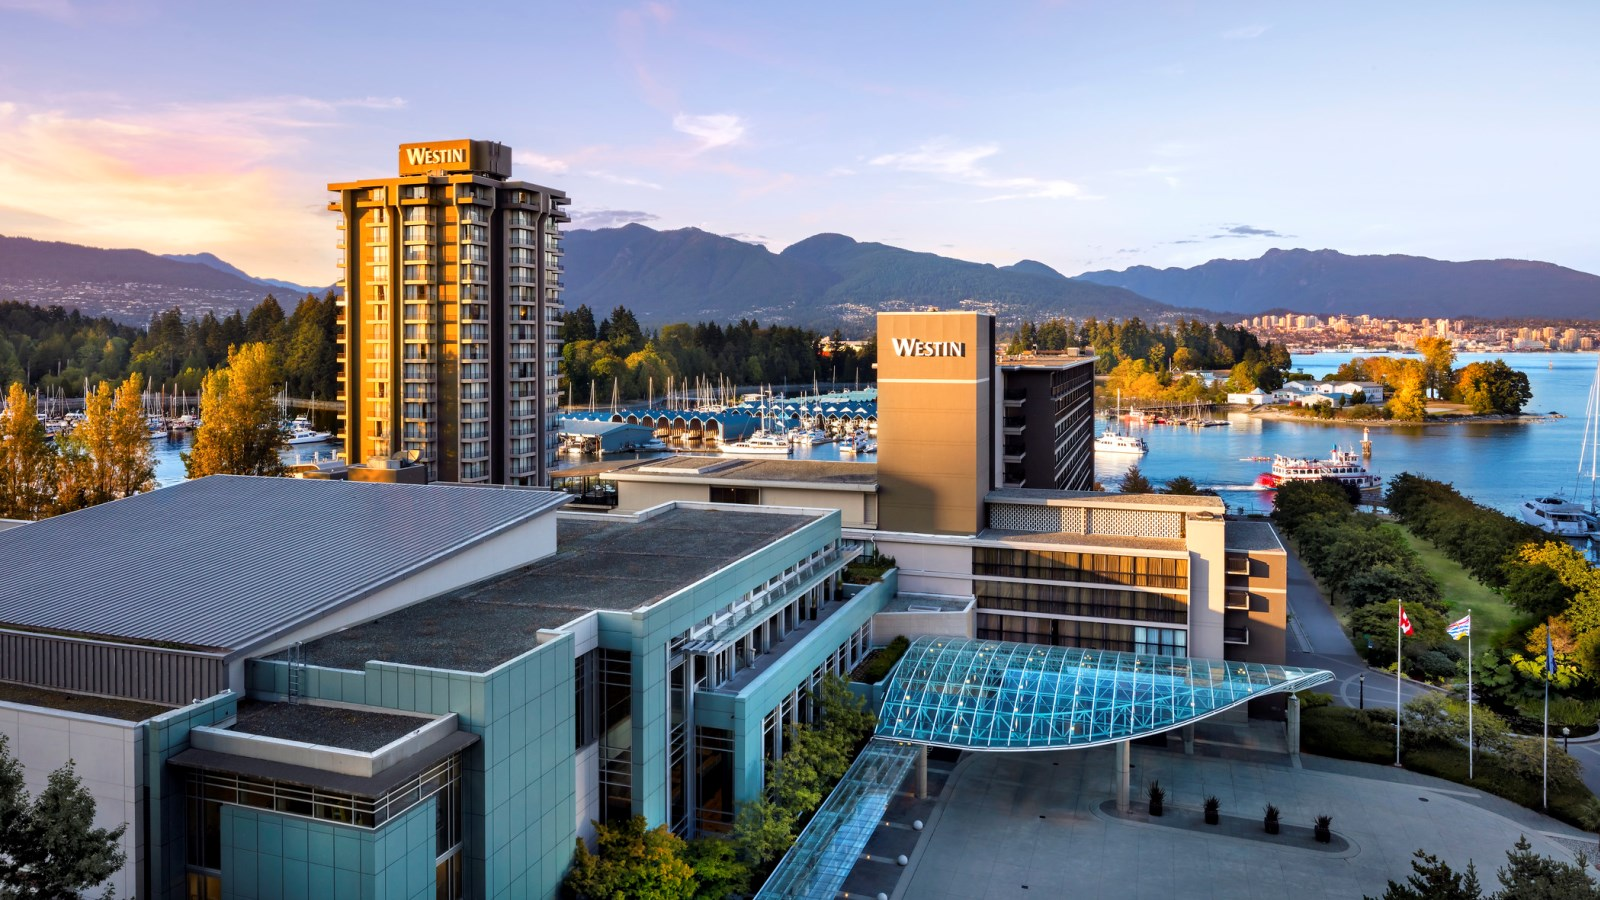
\includegraphics[width=4in]{content/ACL17-westin-bayshore.jpg}

\vspace{2ex}\centerline{\rule{.5\linewidth}{.5pt}}\vspace{2ex}
\setlength{\parskip}{1ex}\setlength{\parindent}{0ex}

\daydateyear, 18:00 -- 21:00 \vspace{1em}\\
Westin Bayshore Hotel (Conference Venue)\\
\WelcomeReceptionLoc\\
\url{http://www.westinbayshore.com/}
\end{center}

\noindent Catch up with your colleagues at the \textbf{Welcome
Reception}! It will be held immediately following the Tutorials
on \daydate at 18:00 in the Bayshore Grand Ballroom of the Westin
Bayshore Hotel (the conference venue). Refreshments and a light
dinner will be provided, and a cash bar will be available.



%% MAIN CONFERENCE %%%%%%%%%%%%%%%%%%%%%%%%%%%%%%%%%%%%%%%%%%%%%%
\newpage
\setdaydateyear{Saturday}{June 2}{2018}
\chapter{Main Conference: \daydate}
\thispagestyle{emptyheader}
\setheaders{Main Conference}{\daydateyear}

%% Overview page %%%%%%%%%%%%%%%%%%%%%%%%%%%%%%%%%%%%%%%%%%%%%%%%
\section*{Overview}
\renewcommand{\arraystretch}{1.2}
\begin{SingleTrackSchedule}
  07:30 & -- & 08:45 &
  {\bfseries Breakfast}
  {\hfill \emph{Empire Foyer}}
  \\
  08:45 & -- & 09:00 &
  {\bfseries Welcome from the Chairs}
  {\hfill \emph{Empire Ballroom }}
  \\
  09:00 & -- & 10:00 &
  {\bfseries Session Keynote: Keynote 1}
  {\hfill \emph{Empire Ballroom }}
  \\
  10:00 & -- & 10:30 &
  {\bfseries Morning Coffee}
  {\hfill \emph{Empire Foyer}}
  \\
  10:30 & -- & 11:30 &
  \begin{tabular}{|p{0.6in}|p{0.6in}|p{0.6in}|p{0.7in}|p{0.7in}|} \hline
    \multicolumn{3}{|l|}{{\bfseries Rsrch. Oral 1/2}} & {\bfseries Indus. Oral 1/2} & {\bfseries Poster/Demo 1 (10:30-12:00)}\\\hline
    Information Extraction 1 & Phonology Morphology and Word Segmentation & Speech & Machine Learning -- Classification & NLP Applications / Discourse and Pragmatics / Generation\\
\emph{Empire A } & \emph{Empire B } & \emph{Empire C } & \emph{Empire D } & \\
    \cline{1-4}\end{tabular} \\
    11:30 & -- & 12:30 &
  \begin{tabular}{|p{0.6in}|p{0.6in}|p{0.6in}|p{0.7in}|p{0.7in}|}
Machine Learning 1 & Information Extraction 2 & Machine Translation & Dialog & \\
\emph{Empire A } & \emph{Empire B } & \emph{Empire C } & \emph{Empire D } & \emph{Elite Hall B}\\
  \hline\end{tabular} \\
  12:30 & -- & 14:00 &
  {\bfseries Lunch}
  \\
  14:00 & -- & 15:00 &
  {\bfseries Industry Track Keynote}
  {\hfill \emph{Empire Ballroom}}
  \\
  15:00 & -- & 15:30 &
  {\bfseries Afternoon Coffee}
  {\hfill \emph{Empire Foyer}}
  \\
  15:30 & -- & 17:00 &
  \begin{tabular}{|p{0.6in}|p{0.6in}|p{0.6in}|p{0.7in}|p{0.7in}|} \hline
    \multicolumn{3}{|l|}{{\bfseries Rsrch. Oral 3}} & {\bfseries Indus. Oral 3} & {\bfseries Poster/Demo 3}\\\hline
 Machine Learning 2 & Social Media and Computational Social Science 1 & Vision, Robotics and Other Grounding 1 & Keynote & Semantics / Sentiment Analysis \\
\emph{Empire A} & \emph{Empire B } & \emph{Empire C } & \emph{Empire D} & \emph{Elite Hall B} \\
  \hline\end{tabular} \\
  17:00 & -- & 18:30 &
  \begin{tabular}{|p{0.8in}|p{0.8in}|p{0.8in}|p{0.85in}|}
    \multicolumn{3}{|l|}{{\bfseries Rsrch. Oral 4}} & {\bfseries Indus. Oral 4}\\ \hline
  NLP Applications & Question Answering & SRW highlight papers & Machine Translation \\
         \emph{Empire A} &         \emph{Empire B } &           \emph{Empire C } & \emph{Empire D } \\
  \hline\end{tabular} \\
\end{SingleTrackSchedule}
\clearpage

%% Invited talk and other events %%%%%%%%%%%%%%%%%%%%%%%%%%%%%%%%
\section{Keynote Address: Charles Yang}
\index{Yang, Charles}

\begin{center}
\begin{Large}
{\bfseries\Large Why 72?}\vspace{1em}\par
\end{Large}

\daydateyear, 9:00--10:00 \vspace{1em}\\
\PlenaryLoc \\
\vspace{1em}\par
\end{center}

\noindent
{\bfseries Biography:} Charles is a Professor of Linguistics, Computer Science, and Psychology at the University of Pennsylvania and directs the Program in Cognitive Science. He has spent a long time to work out the tricks children use to learn languages and is now ready to try them out on machines. His most recent book, The Price of Linguistic Productivity, is the winner of the 2017 LSA Leonard Bloomfield award.

\vspace{2ex}\centerline{\rule{.5\linewidth}{.5pt}}\vspace{2ex}
\setlength{\parskip}{1ex}\setlength{\parindent}{0ex}

\section{Keynote Address: Mari Ostendorf}
\index{Ostendorf, Mari}

\begin{center}
\begin{Large}
{\bfseries\Large TBD}\vspace{1em}\par
\end{Large}

\daydateyear, 14:00--15:00 \vspace{1em}\\
\PlenaryLoc \\
\vspace{1em}\par
\end{center}

\noindent
{\bfseries Biography:} Mari is a professor of Electrical Engineering and Associate Vice Provost for Research at the University of Washington. She is a Fellow of IEEE and ISCA, and winner of the 2018 IEEE James L. Flanagan Speech and Audio Processing Award. Her recent research has emphasized social communication, and she served as a faculty advisor for the student team winning the inaugural AlexaPrize competition to build a socialbot.


\newpage
\clearpage

%% Sessions  %%%%%%%%%%%%%%%%%%%%%%%%%%%%%%%%%%%%%%%%%%%%%%%%%%%%
% \clearpage
\setheaders{Session 1}{\daydateyear}
\begin{SessionOverview}{Session 1}{\daydateyear}{Information Extraction 1}{Phonology Morphology and Word Segmentation}{Speech}{Machine Learning -- Classification}{Posters and Demos}
  \marginnote{\rotatebox{90}{10:30}}[2mm]
  \papertableentry{papers-069} & \papertableentry{papers-044} & \papertableentry{papers-199} & \papertableentry{naacl-2018-industrial-track-1749} & \multirow{3}{*}{\rotatebox[origin=c]{90}{ Discourse and Pragmatics / Generation / NLP Applications}}
  \\
  \cline{1-4}
  \marginnote{\rotatebox{90}{10:48}}[2mm]
  \papertableentry{papers-165} & \papertableentry{papers-094} & \papertableentry{papers-430} & \papertableentry{naacl-2018-industrial-track-1751} & 
  \\
  \cline{1-4}
  \marginnote{\rotatebox{90}{11:06}}[2mm]
  \papertableentry{papers-309} & \papertableentry{papers-136} & \papertableentry{papers-596} & \papertableentry{naacl-2018-industrial-track-1769} &
  \\

\end{SessionOverview}
% \begin{SessionOverview}{Session 1}{\daydateyear}
%   {Oral: Information Extraction 1}
%   {Oral: Phonology Morphology and Word Segmentation}
%   {Oral: Speech}
%   {Machine Learning -- Classification}
%   {Posters}


% \end{SessionOverview}  

\newpage
\section*{Parallel Session 1}
{\bfseries\large Session 1A: Oral: Information Extraction 1}\\
\TrackALoc\hfill\sessionchair{Dan}{Bikel}
\paperabstract{\day}{10:30--10:47}{}{}{papers-069}
\paperabstract{\day}{10:48--11:05}{}{}{papers-165}
\paperabstract{\day}{11:06--11:23}{}{}{papers-309}
\clearpage
{\bfseries\large Session 1B: Oral: Phonology Morphology and Word Segmentation}\\
\TrackBLoc\hfill\sessionchair{Barbara}{Plank}
\paperabstract{\day}{10:30--10:47}{}{}{papers-044}
\paperabstract{\day}{10:48--11:05}{}{}{papers-094}
\paperabstract{\day}{11:06--11:23}{}{}{papers-136}
\clearpage
{\bfseries\large Session 1C: Oral: Speech}\\
\TrackCLoc\hfill\sessionchair{Dilek}{Hakkani-Tur}
\paperabstract{\day}{10:30--10:47}{}{}{papers-199}
\paperabstract{\day}{10:48--11:05}{}{}{papers-430}
\paperabstract{\day}{11:06--11:23}{}{}{papers-596}
\clearpage
{\bfseries\large Session 1D: Machine Learning -- Classification}\\
\TrackDLoc\hfill\sessionchair{Luke}{Zettlemoyer}
\paperabstract{\day}{10:30--10:50}{}{}{naacl-2018-industrial-track-1749}
\paperabstract{\day}{10:50--11:10}{}{}{naacl-2018-industrial-track-1751}
\paperabstract{\day}{11:10--11:30}{}{}{naacl-2018-industrial-track-1769}
\clearpage



% \clearpage
\setheaders{Session 2}{\daydateyear}
\begin{ThreeSessionOverview}{Session 2}{\daydateyear}
  {Oral: Machine Learning 1}
  {Oral: Information Extraction 2}
  {Oral: Machine Translation 1}
  {Dialog}
  \marginnote{\rotatebox{90}{11:30}}[2mm]
  \papertableentry{papers-279} & \papertableentry{papers-486} & \papertableentry{papers-078} & \papertableentry{naacl-2018-industrial-track-1716}
  \\
  \hline
  \marginnote{\rotatebox{90}{11:48}}[2mm]
  \papertableentry{papers-309} & \papertableentry{papers-520} & \papertableentry{papers-446} & \papertableentry{naacl-2018-industrial-track-1762}
  \\
  \hline
  \marginnote{\rotatebox{90}{12:06}}[2mm]
  \papertableentry{tacl-449} & \papertableentry{tacl-450} & \papertableentry{papers-458} & \papertableentry{naacl-2018-industrial-track-1788}
  \\
\end{ThreeSessionOverview}

\newpage
\section*{Parallel Session 2}
{\bfseries\large Session 2A: Oral: Machine Learning 1}\\
\TrackALoc\hfill\sessionchair{Raymond}{Mooney}
\paperabstract{\day}{11:30--11:48}{}{}{papers-279}
\paperabstract{\day}{11:48--12:06}{}{}{papers-309}
\paperabstract{\day}{12:06--12:24}{}{}{tacl-449}
\clearpage
{\bfseries\large Session 2B: Oral: Information Extraction 2}\\
\TrackBLoc\hfill\sessionchair{Mihai}{Surdeanu}
\paperabstract{\day}{11:30--11:48}{}{}{papers-486}
\paperabstract{\day}{11:48--12:06}{}{}{papers-520}
\paperabstract{\day}{12:06--12:24}{}{}{tacl-450}
\clearpage
{\bfseries\large Session 2C: Oral: Machine Translation 1}\\
\TrackCLoc\hfill\sessionchair{Daniel}{Marcu}
\paperabstract{\day}{11:30--11:48}{}{}{papers-078}
\paperabstract{\day}{11:48--12:06}{}{}{papers-446}
\paperabstract{\day}{12:06--12:24}{}{}{papers-458}
\clearpage
{\bfseries\large Session 2D: Dialog}\\
\TrackDLoc\hfill\sessionchair{Christine}{Doran}
\paperabstract{\day}{11:30--11:47}{}{}{naacl-2018-industrial-track-1716}
\paperabstract{\day}{11:48--12:05}{}{}{naacl-2018-industrial-track-1762}
\paperabstract{\day}{12:05--12:23}{}{}{naacl-2018-industrial-track-1788}
\clearpage



% \clearpage
\setheaders{Session 3}{\daydateyear}
\begin{ThreeSessionOverview}{Session 3}{\daydateyear}
  {Oral: Machine Learning 2}
  {Oral: Social Media and Computational Social Science 1}
  {Oral: Vision, Robotics and Other Grounding 1}
  \marginnote{\rotatebox{90}{15:30}}[2mm]
  \papertableentry{papers-182} & \papertableentry{papers-282} & \papertableentry{papers-171}
  \\
  \hline
  \marginnote{\rotatebox{90}{15:48}}[2mm]
  \papertableentry{papers-1039} & \papertableentry{papers-445} & \papertableentry{papers-225}
  \\
  \hline
  \marginnote{\rotatebox{90}{16:06}}[2mm]
  \papertableentry{tacl-451} & \papertableentry{papers-710} & \papertableentry{papers-260}
  \\
  \hline
  \marginnote{\rotatebox{90}{16:24}}[2mm]
  \papertableentry{tacl-452} & \papertableentry{tacl-453} & \papertableentry{papers-272}
  \\
\end{ThreeSessionOverview}

\newpage
\section*{Parallel Session 3}
{\bfseries\large Session 3A: Oral: Machine Learning 2}\\
\TrackALoc\hfill\sessionchair{}{}
\paperabstract{\day}{15:30--15:47}{}{}{papers-182}
\paperabstract{\day}{15:48--16:05}{}{}{papers-1039}
\paperabstract{\day}{16:06--16:24}{}{}{tacl-451}
\paperabstract{\day}{16:24--16:42}{}{}{tacl-452}
\clearpage
{\bfseries\large Session 3B: Oral: Social Media and Computational Social Science 1}\\
\TrackBLoc\hfill\sessionchair{Margaret}{Mitchell (moved!!)}
\paperabstract{\day}{15:30--15:47}{}{}{papers-282}
\paperabstract{\day}{15:48--16:05}{}{}{papers-445}
\paperabstract{\day}{16:06--16:23}{}{}{papers-710}
\paperabstract{\day}{16:24--16:42}{}{}{tacl-453}
\clearpage
{\bfseries\large Session 3C: Oral: Vision, Robotics and Other Grounding 1}\\
\TrackCLoc\hfill\sessionchair{Mirella}{Lapata}
\paperabstract{\day}{15:30--15:47}{}{}{papers-171}
\paperabstract{\day}{15:48--16:05}{}{}{papers-225}
\paperabstract{\day}{16:06--16:23}{}{}{papers-260}
\paperabstract{\day}{16:24--16:42}{}{}{papers-272}
\clearpage



% \clearpage
\setheaders{Session 4}{\daydateyear}
\begin{ThreeSessionOverview}{Session 4}{\daydateyear}
  {Oral: NLP Applications}
  {Oral: Question Answering}
  {Oral: SRW highlight papers}
  {Machine Translation}
  \marginnote{\rotatebox{90}{17:00}}[2mm]
  \papertableentry{papers-415} & \papertableentry{papers-018} & \papertableentry{naacl2018-SRW-3031} & \papertableentry{naacl-2018-industrial-track-1731}
  \\
  \hline
  \marginnote{\rotatebox{90}{17:18}}[2mm]
  \papertableentry{papers-498} & \papertableentry{papers-051} & \papertableentry{naacl2018-SRW-3009} & \papertableentry{naacl-2018-industrial-track-1744}
  \\
  \hline
  \marginnote{\rotatebox{90}{17:36}}[2mm]
  \papertableentry{papers-609} & \papertableentry{papers-116} & \papertableentry{naacl2018-SRW-3040} & \papertableentry{naacl-2018-industrial-track-1754}
  \\
  \hline
  \marginnote{\rotatebox{90}{18:13}}[2mm]
  \papertableentry{papers-980} & \papertableentry{papers-082} & \papertableentry{naacl2018-SRW-3051} & \papertableentry{naacl-2018-industrial-track-1786}
  \\
  \hline
  \marginnote{\rotatebox{90}{17:54}}[2mm]
  \papertableentry{tacl-455} & \papertableentry{tacl-456} & \papertableentry{naacl2018-SRW-3053} & 
  \\
\end{ThreeSessionOverview}

\newpage
\section*{Parallel Session 4}
{\bfseries\large Session 4A: Oral: NLP Applications}\\
\TrackALoc\hfill\sessionchair{Yang}{Liu}
\paperabstract{\day}{17:00--17:17}{}{}{papers-415}
\paperabstract{\day}{17:18--17:35}{}{}{papers-498}
\paperabstract{\day}{17:36--17:53}{}{}{papers-609}
\paperabstract{\day}{18:13--18:30}{}{}{papers-980}
\paperabstract{\day}{17:54--18:13}{}{}{tacl-455}
\clearpage
{\bfseries\large Session 4B: Oral: Question Answering}\\
\TrackBLoc\hfill\sessionchair{Eugene}{Agichtein}
\paperabstract{\day}{17:00--17:17}{}{}{papers-018}
\paperabstract{\day}{17:18--17:35}{}{}{papers-051}
\paperabstract{\day}{17:36--17:53}{}{}{papers-116}
\paperabstract{\day}{17:54--18:12}{}{}{papers-082}
\paperabstract{\day}{18:13--18:30}{}{}{tacl-456}
\clearpage
{\bfseries\large Session 4C: Oral: SRW highlight papers}\\
\TrackCLoc\hfill\sessionchair{Umashanthi Pavalanathan}{Shereen Oraby}
\paperabstract{\day}{None}{}{}{naacl2018-SRW-3031}
\paperabstract{\day}{17:00--17:14}{}{}{naacl2018-SRW-3009}
\paperabstract{\day}{17:15--17:29}{}{}{naacl2018-SRW-3040}
\paperabstract{\day}{17:30--17:44}{}{}{naacl2018-SRW-3051}
\paperabstract{\day}{17:45--17:59}{}{}{naacl2018-SRW-3053}
\paperabstract{\day}{18:00--18:14}{}{}{naacl2018-SRW-3030}
\paperabstract{\day}{18:15--18:30}{}{}{naacl2018-SRW-3046}
\clearpage
{\bfseries\large Session 4D: Machine Translation}\\
\TrackDLoc\hfill\sessionchair{Kenneth}{Heafield}
\paperabstract{\day}{17:00--17:17}{}{}{naacl-2018-industrial-track-1731}
\paperabstract{\day}{17:18--17:35}{}{}{naacl-2018-industrial-track-1744}
\paperabstract{\day}{17:36--17:53}{}{}{naacl-2018-industrial-track-1754}
\paperabstract{\day}{17:54--18:12}{}{}{naacl-2018-industrial-track-1786}
\clearpage



%\input{auto/papers/Saturday-Session-P1A.tex}
%\input{auto/papers/Saturday-Session-P1B.tex}
%\input{auto/papers/Saturday-Session-P1C.tex}


\setdaydateyear{Sunday}{June 3}{2018}
\chapter{Main Conference: \daydate}
\thispagestyle{emptyheader}
\setheaders{Main Conference}{\daydateyear}

\newif\ifmetaconf
%\metaconftrue

%% Overview page %%%%%%%%%%%%%%%%%%%%%%%%%%%%%%%%%%%%%%%%%%%%%%%%
%\ifmetaconf
%\addcontentsline{toc}{section}{Discussion: Double Blind Reviewing \& arXiv, 12:05--13:30, \MetaConfLoc}
%\fi
%\input{auto/papers/Tuesday-overview.tex}\clearpage

%% Invited talk and other events %%%%%%%%%%%%%%%%%%%%%%%%%%%%%%%%
\section{Keynote Address: Kevin Knight (sponsored by Google)}
\index{Knight, Kevin}

\begin{center}
\begin{Large}
{\bfseries\Large The Moment When the Future Fell Asleep}\vspace{1em}\par
\end{Large}

\daydateyear, 9:00--10:00 \vspace{1em}\\
\sessionchair{Amanda}{Stent}
\PlenaryLoc \\
\vspace{1em}\par
\end{center}

\vspace{2ex}\centerline{\rule{.5\linewidth}{.5pt}}\vspace{2ex}
\setlength{\parskip}{1ex}\setlength{\parindent}{0ex}


\noindent
{\bfseries Biography:} Kevin is a professor of computer science at the University of Southern California and fellow of the Information Sciences Institute. He is a 2014 fellow of the ACL for foundational contributions to machine translation, to the application of automata for NLP, to decipherment of historical manuscripts, to semantics and to generation.

\vspace{2ex}\centerline{\rule{.5\linewidth}{.5pt}}\vspace{2ex}
\setlength{\parskip}{1ex}\setlength{\parindent}{0ex}

% \section{Industry Keynote Address: Daniel Marcu}
% \index{Marcu, Daniel}

% \begin{center}
% \begin{Large}
% {\bfseries\Large Building innovative startups, products, and services – personal insights}\vspace{1em}\par
% \end{Large}

% \daydateyear, 14:00--15:00 \vspace{1em}\\
% \sessionchair{Jennifer}{Chu-Carroll}
% \PlenaryLoc \\
% \vspace{1em}\par
% \end{center}

% \noindent
% {\bfseries Abstract:} During the last 15 years, NLP\&ML scientists have started to explore with increased persistence how to turn science into successful startups and how to incorporate cutting edge research into innovative products and services. In this talk, I will review lessons learned from my personal experience in this area.

% \noindent
% {\bfseries Biography:} Daniel is a Director of MT/NLP at Amazon. He is a 2014 fellow of ACL for significant contributions to discourse parsing, summarization and machine translation and for kick starting the statistical machine translation industry.


\newpage
\clearpage

%% Sessions  %%%%%%%%%%%%%%%%%%%%%%%%%%%%%%%%%%%%%%%%%%%%%%%%%%%%
% \input{auto/papers/Tuesday-parallel-session-4.tex}
% \input{auto/papers/Tuesday-parallel-session-5.tex}
% \input{auto/papers/Tuesday-parallel-session-6.tex}
% \input{auto/papers/Tuesday-Session-P2A.tex}
% \input{auto/papers/Tuesday-Session-P2B.tex}
% \input{auto/papers/Tuesday-Session-P2C.tex}


%% SOCIAL EVENT %%%%%%%%%%%%%%%%%%%%%%%%%%%%%%%%%%%%%%%%%%%%%%%%%
\newpage
\setheaders{}{}
\addcontentsline{toc}{chapter}{Social Event: \daydate, 18:45}
\clearpage
\section[Social Event]{Social Event}
\setheaders{}{\daydateyear}
\begin{center}

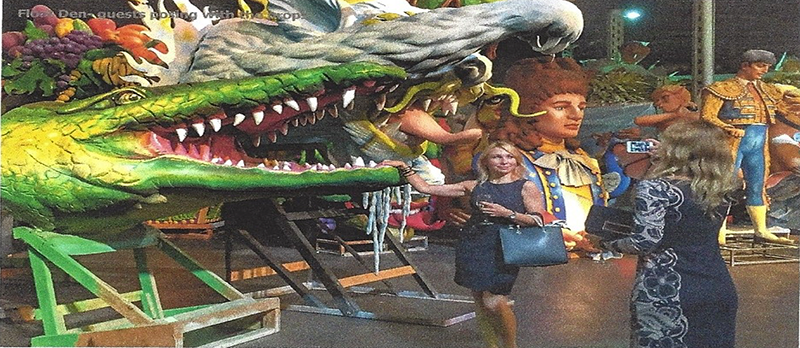
\includegraphics[width=4in]{content/social_event_1.png}

\vspace{2ex}\centerline{\rule{.5\linewidth}{.5pt}}\vspace{2ex}
\setlength{\parskip}{1ex}\setlength{\parindent}{0ex}

\daydateyear, 18:45 -- 21:00 \vspace{1em}\\
Blaine Kern's Mardi Gras World\\
\url{https://www.mardigrasworld.com/}
\end{center}

\noindent Catch the shuttle bus outside of the Hyatt Regency New Orleans, conference hotel, at \textbf{18:45 sharp}. Bus loading will be to the back side of the escalator near the reservation desk.  Please do not be late.  This will take you the short ride to:

\vspace{.25in}

{\huge \textbf{Blaine Kern's Mardi Gras World}}

\vspace{.25in}

\noindent Mardi Gras World is a world of wonders created for you by the people who bring Mardi Gras to life every year—--the artists of Blaine Kern Studios. It’s all in one magical place where you can peek behind the curtain and see Mardi Gras in the making.

\noindent Since 1947, Blaine Kern Studios has been as much a part of Carnival as the parades New Orleans loves. In fact, they create most of those parades, from concept through completion. They are \textbf{the world’s leading makers of floats, sculpture and props}. Their work and props are located in theme parks, casinos and amusement parks around the globe---from here to Shanghai.

\noindent Your event \textbf{begins with a walk-through of the float den} among larger-than-life works of art. Visit The Studio, where you can watch artists designing, carving, painting and building for next year’s parades. Guests will \textbf{explore props of every theme imaginable while enjoying passed hors d'oeuvres and a traditional New Orleans band, complete with a Grand Marshall}.

\noindent Guests will then follow stilt walkers to make their way to the \textbf{dockside River City Plaza} and \textbf{River City Ballroom} for New Orleans' famous cuisine and libations and live \textbf{Zydeco, funk, soul and R\&B from one of the best performers in the city}. This will surely be a night to remember!

% \begin{center}
% 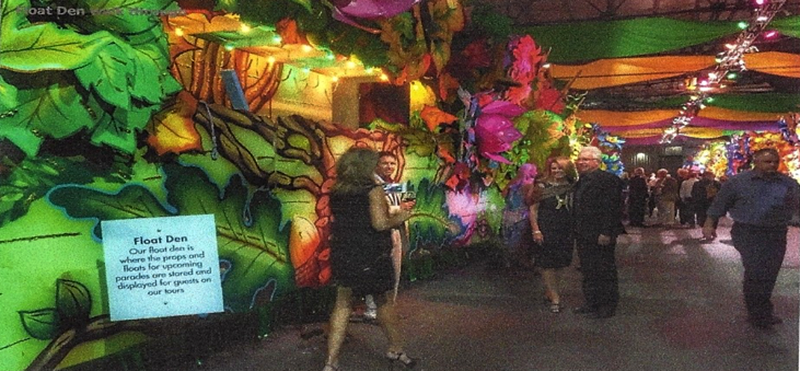
\includegraphics[width=4in]{content/social_event_2.png}
% \end{center}


\setdaydateyear{Monday}{June 4}{2018}
\chapter{Main Conference: \daydate}
\thispagestyle{emptyheader}
\setheaders{Main Conference}{\daydateyear}

%% Overview page %%%%%%%%%%%%%%%%%%%%%%%%%%%%%%%%%%%%%%%%%%%%%%%%
\section*{Overview}
\renewcommand{\arraystretch}{1.2}
\begin{SingleTrackSchedule}
  07:30 & -- & 18:00 &
  {\bfseries Registration}
  \hfill\emph{\RegistrationLoc}
  \\
  07:45 & -- & 08:45 &
  {\bfseries Breakfast}
  {\hfill \emph{Empire Foyer}}
  \\
  08:45 & -- & 09:00 &
  {\bfseries Announcements}
  {\hfill \emph{Empire Ballroom }}
  \\
  09:00 & -- & 10:00 &
  {\bfseries Keynote Address: Dilek Hakkani-Tür (sponsored by Bloomberg)}
  {\hfill \emph{Empire Ballroom }}
  \\
  10:00 & -- & 10:30 &
  {\bfseries Morning Coffee}
  {\hfill \emph{Empire Foyer}}
  \\
  10:30 & -- & 11:30 &
  \begin{tabular}{|p{0.6in}|p{0.6in}|p{0.6in}|p{0.7in}|p{0.7in}|} \cline{1-3}\cline{5-5}
    \multicolumn{3}{|l|}{{\bfseries Research Oral 9}} &  & {\bfseries Poster/Demo 9/10 (10:30-12:00)}\\\cline{1-3}
Information Extraction 4 & Semantics 4 & Generation 2 & & \multirow{2}{0.7in}{\small{Question Answering 2 / Social Media \& Computational Social Science 3 / Summarization 2 / Demos}} \\
\emph{Empire A } & \emph{Empire B } & \emph{Empire C } & &\\
  \end{tabular} \\
11:30 & -- & 12:30 &
\begin{tabular}{|p{0.6in}|p{0.6in}|p{0.6in}|p{0.7in}|p{0.7in}|} \cline{1-4}
      \multicolumn{3}{|l|}{{\bfseries Research Oral 10}} & {\bfseries Industry Oral 10} & \\\cline{1-4}
Dialogue and Interactive Systems 1 & Information Extraction 5 & Generation 3 & Machine Learning - Prediction & \\
\emph{Empire A } & \emph{Empire B } & \emph{Empire C } & \emph{Empire D} & \emph{Elite Hall B}\\
  \hline\end{tabular} \\
  12:30 & -- & 14:00 &
  {\bfseries Lunch}
  \\
  13:00 & -- & 14:00 &
  {\bfseries NAACL Business Meeting}
  \\
  14:00 & -- & 15:30 &
  \begin{tabular}{|p{0.8in}|p{0.8in}|p{0.8in}|p{0.8in}|} \hline
        \multicolumn{3}{|l|}{{\bfseries Research Oral 11}} & {\bfseries Poster/Demo 11}\\\hline
Sentiment Analysis 2 & Discourse and Pragmatics 2 & Tagging, Chunking, Syntax and Parsing 3 & \footnotesize{Cognitive Modeling and Psycholinguistics 2 / Dialogue and Interactive Systems 2 / Text Mining 2 / Speech 2 / Vision, Robotics and Other Grounding 3 / Demos} \\
\emph{Empire A } & \emph{Empire B } & \emph{Empire C } & \emph{Elite Hall B } \\
  \hline\end{tabular} \\
  15:30 & -- & 16:00 &
  {\bfseries Afternoon Coffee}
  {\hfill \emph{Empire Foyer}}
  \\
  17:00 & -- & 18:15 &
  {\bfseries Outstanding Papers and Closing Session}
  {\hfill \emph{Empire Ballroom }}
  \\
\end{SingleTrackSchedule}
\clearpage

%% Invited talk and other events %%%%%%%%%%%%%%%%%%%%%%%%%%%%%%%%
\section{Keynote Address: Dilek Hakkani-T\"{u}r}
\index{Hakkani-T\"{u}r, Dilek}

\begin{center}
\begin{Large}
{\bfseries\Large Google Assistant or My Assistant? Towards Personalized Situated Conversational Agents}\vspace{1em}\par
\end{Large}

\daydateyear, 9:00--10:10 \vspace{1em}\\
\PlenaryLoc \\
\vspace{1em}\par
\end{center}

\noindent
{\bfseries Abstract:} Interacting with machines in natural language has been a holy grail since the beginning of computers. Given the difficulty of understanding natural language, only in the past couple of decades, we started seeing real user applications for targeted/limited domains. More recently, advances in deep learning based approaches enabled exciting new research frontiers for end-to-end goal-oriented conversational systems. However, personalization (i.e., learning to take actions from users and learning about users beyond memorizing simple attributes) remains a research challenge. In this talk, I’ll review end-to-end situated dialogue systems research, with components for situated language understanding, dialogue state tracking, policy, and language generation. The talk will highlight novel approaches where dialogue is viewed as a collaborative game between a user and an agent in the presence of visual information. The situated conversational agent can be bootstrapped using user simulation (crawl), improved through interactions with crowd-workers (walk), and iteratively refined with real user interactions (run).

\vspace{2ex}\centerline{\rule{.5\linewidth}{.5pt}}\vspace{2ex}
\setlength{\parskip}{1ex}\setlength{\parindent}{0ex}

% \vspace{3em}\par 
% \vfill

\noindent
{\bfseries Biography:} Dilek is a research scientist at Google Research Dialogue Group and has previously held positions at Microsoft Research, ICSI, and AT\&T Labs – Research. She is a fellow of the IEEE and of ISCA. Her research interests include conversational AI, natural language and speech processing, spoken dialogue systems, and machine learning for language processing.

\newpage
\clearpage

\clearpage
\setheaders{Session 9}{\daydateyear}
\begin{FourSessionOverview}{Session 9}{\daydateyear}
  {Information Extraction 4}
  {Semantics 4}
  {Generation 2}
  {Posters and Demos(10:30--12:00)}
  \marginnote{\rotatebox{90}{10:30}}[2mm]
  \papertableentry{papers-444} & \papertableentry{papers-426} & \papertableentry{papers-365} & 
  \\
  \cline{1-3}
  \marginnote{\rotatebox{90}{10:48}}[2mm]
  \papertableentry{papers-477} & \papertableentry{papers-539} & \papertableentry{papers-381} & \multirow{5}{1in}{Question Answering 2 / Social Media \& Computational Social Science 3 / Summarization 2 / Demos}
  \\
  \cline{1-3}
  \marginnote{\rotatebox{90}{11:06}}[2mm]
  \papertableentry{papers-485} & \papertableentry{papers-608} & \papertableentry{papers-548} &
  \\
\end{FourSessionOverview}

\newpage
\section*{Parallel Session 9}
\subsection{Information Extraction 4}
\TrackALoc\hfill\sessionchair{Bonan}{Min}
\paperabstract{\day}{10:30--10:48}{}{}{papers-444}
\paperabstract{\day}{10:48--11:06}{}{}{papers-477}
\paperabstract{\day}{11:06--11:24}{}{}{papers-485}
\clearpage
\subsection{Semantics 4}
\TrackBLoc\hfill\sessionchair{Yoav}{Artzi}
\paperabstract{\day}{10:30--15:48}{}{}{papers-426}
\paperabstract{\day}{10:48--11:06}{}{}{papers-539}
\paperabstract{\day}{11:06--11:24}{}{}{papers-608}
\clearpage
\subsection{Generation 2}
\TrackCLoc\hfill\sessionchair{Michael}{White}
\paperabstract{\day}{10:30--10:48}{}{}{papers-365}
\paperabstract{\day}{10:48--11:06}{}{}{papers-381}
\paperabstract{\day}{11:06--11:24}{}{}{papers-548}
\clearpage



\clearpage
\setheaders{Session 10}{\daydateyear}
\begin{SessionOverview}{Session 10}{\daydateyear}
  {Dialogue and Interactive Systems 1}
  {Information Extraction 5}
  {Generation 3}
  {Industry: Machine Learning - Prediction}
  {Posters and Demos (10:30--12:00)}
  \marginnote{\rotatebox{90}{11:30}}[2mm]
  \papertableentry{papers-033} & \papertableentry{papers-570} & \papertableentry{papers-566} & \papertableentry{naacl-2018-industrial-track-1742} &
  \\
  \cline{1-4}
  \marginnote{\rotatebox{90}{11:48}}[2mm]
  \papertableentry{papers-132} & \papertableentry{papers-623} & \papertableentry{papers-602} & \papertableentry{naacl-2018-industrial-track-1750} & \multirow{5}{.8in}{Question Answering 2 / Social Media \& Computational Social Science 3 / Summarization 2 / Demos}
  \\
  \cline{1-4}
  \marginnote{\rotatebox{90}{12:06}}[2mm]
  \papertableentry{papers-192} & \papertableentry{papers-657} & \papertableentry{papers-640} & \papertableentry{naacl-2018-industrial-track-1782} &
  \\
\end{SessionOverview}

\newpage
\section*{Parallel Session 10}
\subsection{Oral: Dialogue and Interactive Systems 1}
\TrackALoc\hfill\sessionchair{Yun-Nung}{Chen}
\paperabstract{\day}{11:30--11:47}{}{}{papers-033}
\paperabstract{\day}{11:48--12:05}{}{}{papers-132}
\paperabstract{\day}{12:06--12:23}{}{}{papers-192}
\clearpage
\subsection{Oral: Information Extraction 5}
\TrackBLoc\hfill\sessionchair{Xiang}{Ren}
\paperabstract{\day}{11:30--11:47}{}{}{papers-570}
\paperabstract{\day}{11:48--12:05}{}{}{papers-623}
\paperabstract{\day}{12:06--12:23}{}{}{papers-657}
\clearpage
\subsection{Oral: Generation 3}
\TrackCLoc\hfill\sessionchair{Amanda}{Stent}
\paperabstract{\day}{11:30--11:47}{}{}{papers-566}
\paperabstract{\day}{11:48--12:05}{}{}{papers-602}
\paperabstract{\day}{12:06--12:23}{}{}{papers-640}
\clearpage
\subsection{Industry: Machine Learning - Prediction}
\TrackDLoc\hfill\sessionchair{Gokhan}{Tur}
\paperabstract{\day}{11:30--11:47}{}{}{naacl-2018-industrial-track-1742}
\paperabstract{\day}{11:48--12:05}{}{}{naacl-2018-industrial-track-1750}
\paperabstract{\day}{12:06--12:23}{}{}{naacl-2018-industrial-track-1782}
\clearpage


\section*{Posters and Demos: Sessions 9/10}

\subsection{Posters: Question Answering 2}
\setheaders{Sessions 9/10: Posters and Demos: Question Answering 2}{\daydateyear}
Time: \emph{10:30--12:00}\hfill Location: \PosterLoc\\
\sessionchair{Lu}{Wang}
\posterabstract{papers-420}
\posterabstract{papers-702}
\posterabstract{papers-990}
\posterabstract{papers-191}
\posterabstract{papers-348}
\posterabstract{papers-705}
\posterabstract{papers-1074}
\posterabstract{papers-1085}
\posterabstract{papers-109}
\posterabstract{papers-368}
\posterabstract{papers-878}
\posterabstract{naacl2018-SRW-3043}

\subsection{Posters: Social Media and Computational Social Science 3}
\setheaders{Sessions 9/10: Posters and Demos: Social Media and Computational Social Science 3}{\daydateyear}
Time: \emph{10:30--12:00}\hfill Location: \PosterLoc\\
\sessionchair{Lu}{Wang}
\posterabstract{papers-198}
\posterabstract{papers-930}
\posterabstract{papers-789}
\posterabstract{papers-306}
\posterabstract{papers-338}
\posterabstract{papers-122}
\posterabstract{papers-723}
\posterabstract{papers-492}
\posterabstract{naacl2018-SRW-3028}

\subsection{Posters: Summarization 2}
\setheaders{Sessions 9/10: Posters and Demos: Summarization 2}{\daydateyear}
Time: \emph{10:30--12:00}\hfill Location: \PosterLoc\\
\sessionchair{Lu}{Wang}
\posterabstract{papers-086}
\posterabstract{papers-910}
\posterabstract{papers-1064}
\posterabstract{papers-582}
\posterabstract{papers-1029}
\posterabstract{papers-213}
\posterabstract{papers-665}
\posterabstract{papers-007}
\posterabstract{papers-118}
\posterabstract{papers-380}
\posterabstract{papers-1089}
\posterabstract{papers-971}
\posterabstract{papers-1045}
\posterabstract{papers-239}
\posterabstract{papers-861}
\posterabstract{papers-226}
\posterabstract{papers-1081}
\posterabstract{papers-241}
\posterabstract{papers-568}
\posterabstract{papers-715}
\posterabstract{papers-073}
\posterabstract{papers-1000}
\posterabstract{papers-490}

\subsection{Demos}
\setheaders{Sessions 9/10: Posters and Demos: Demos}{\daydateyear}
Time: \emph{10:30--12:00}\hfill Location: \PosterLoc\\

\posterabstract{naacl2018-demos-1502}
\posterabstract{naacl2018-demos-1525}


\clearpage
\setheaders{Session 11}{\daydateyear}
\begin{FourSessionOverview}{Session 11}{\daydateyear}
  {Sentiment Analysis 2}
  {Discourse and Pragmatics 2}
  {Tagging, Chunking, Syntax and Parsing 3}
  {Posters and Demos}
  \marginnote{\rotatebox{90}{14:00}}[2mm]
  \papertableentry{papers-289} & \papertableentry{papers-143} & \papertableentry{papers-743} &
  \\
  \cline{1-3}
  \marginnote{\rotatebox{90}{14:18}}[2mm]
  \papertableentry{papers-388} & \papertableentry{papers-367} & \papertableentry{papers-672} &
  \\
  \cline{1-3}
  \marginnote{\rotatebox{90}{14:36}}[2mm]
  \papertableentry{papers-606} & \papertableentry{papers-440} & \papertableentry{tacl-462} & \multirow{5}{1in}{Cognitive Modeling and Psycholinguistics 2 / Dialogue and Interactive Systems 2 / Text Mining 2 / Speech 2 / Vision, Robotics and Other Grounding 3 / Demos}
  \\
  \cline{1-3}
  \marginnote{\rotatebox{90}{14:54}}[2mm]
  \papertableentry{papers-627} & \papertableentry{papers-604} & \papertableentry{tacl-463} &
  \\
  \cline{1-3}
  \marginnote{\rotatebox{90}{15:12}}[2mm]
  \papertableentry{papers-854} & \papertableentry{papers-972} & \papertableentry{tacl-464} &
  \\
\end{FourSessionOverview}

\newpage
\section*{Parallel Session 11}
\subsection{Oral: Sentiment Analysis 2}
\TrackALoc\hfill\sessionchair{Smaranda}{Muresan}
\paperabstract{\day}{14:00--14:17}{}{}{papers-289}
\paperabstract{\day}{14:18--14:35}{}{}{papers-388}
\paperabstract{\day}{14:36--14:53}{}{}{papers-606}
\paperabstract{\day}{14:54--15:12}{}{}{papers-627}
\paperabstract{\day}{15:13--15:30}{}{}{papers-854}
\clearpage
\subsection{Oral: Discourse and Pragmatics 2}
\TrackBLoc\hfill\sessionchair{Vincent}{Ng}
\paperabstract{\day}{14:00--14:17}{}{}{papers-143}
\paperabstract{\day}{14:18--14:35}{}{}{papers-367}
\paperabstract{\day}{14:36--14:53}{}{}{papers-440}
\paperabstract{\day}{14:54--15:12}{}{}{papers-604}
\paperabstract{\day}{15:13--15:30}{}{}{papers-972}
\clearpage
\subsection{Oral: Tagging, Chunking, Syntax and Parsing 3}
\TrackCLoc\hfill\sessionchair{Thamar}{Solorio}
\paperabstract{\day}{14:00--14:17}{}{}{tacl-462}
\paperabstract{\day}{14:18--14:35}{}{}{tacl-463}
\paperabstract{\day}{14:36--14:53}{}{}{tacl-464}
\paperabstract{\day}{14:54--15:12}{}{}{papers-743}
\paperabstract{\day}{15:13--15:30}{}{}{papers-672}
\clearpage

\section*{Posters and Demos: Session 11}
\subsection{Posters: Cognitive Modeling and Psycholinguistics 2}
\setheaders{Session 11: Posters and Demos: Cognitive Modeling and Psycholinguistics 2}{\daydateyear}
Time: \emph{14:00--15:30}\hfill Location: \PosterLoc\\
\sessionchair{Hannaneh}{Hajishirzi}
\posterabstract{papers-290}
\posterabstract{papers-560}
\posterabstract{papers-1063}
\posterabstract{papers-449}
\posterabstract{papers-467}
\posterabstract{papers-409}
\posterabstract{naacl2018-SRW-3034}


\subsection{Posters: Dialogue and Interactive Systems 2}
\setheaders{Session 11: Posters and Demos: Dialogue and Interactive Systems 2}{\daydateyear}
Time: \emph{14:00--15:30}\hfill Location: \PosterLoc\\
\sessionchair{Hannaneh}{Hajishirzi}
\posterabstract{papers-613}
\posterabstract{papers-856}
\posterabstract{papers-299}
\posterabstract{papers-218}
\posterabstract{papers-804}
\posterabstract{papers-621}

\subsection{Posters: Text Mining 2}
\setheaders{Session 11: Posters and Demos: Text Mining 2}{\daydateyear}
Time: \emph{14:00--15:30}\hfill Location: \PosterLoc\\
\sessionchair{Hannaneh}{Hajishirzi}
\posterabstract{papers-421}
\posterabstract{papers-768}
\posterabstract{papers-866}
\posterabstract{papers-125}
\posterabstract{papers-855}
\posterabstract{papers-905}

\subsection{Posters: Speech 2}
\setheaders{Session 11: Posters and Demos: Speech 2}{\daydateyear}
Time: \emph{14:00--15:30}\hfill Location: \PosterLoc\\
\sessionchair{Hannaneh}{Hajishirzi}
\posterabstract{papers-322}
\posterabstract{papers-072}
\posterabstract{papers-276}
\posterabstract{papers-986}
\posterabstract{papers-904}
\posterabstract{papers-084}

\subsection{Posters: Vision, Robotics and Other Grounding 3}
\setheaders{Session 11: Posters and Demos: Vision, Robotics and Other Grounding 3}{\daydateyear}
Time: \emph{14:00--15:30}\hfill Location: \PosterLoc\\
\sessionchair{Hannaneh}{Hajishirzi}
\posterabstract{papers-970}
\posterabstract{papers-526}
\posterabstract{papers-726}
\posterabstract{papers-185}
\posterabstract{papers-644}
\posterabstract{papers-840}
\posterabstract{papers-461}
\posterabstract{papers-540}
\posterabstract{papers-081}
\posterabstract{papers-718}
\posterabstract{papers-1002}
\posterabstract{papers-1008}
\posterabstract{papers-1042}
\posterabstract{naacl2018-SRW-3010}

\subsection{Demos}
\setheaders{Session 11: Posters and Demos: Demos}{\daydateyear}
Time: \emph{14:00--15:30}\hfill Location: \PosterLoc\\

\posterabstract{naacl2018-demos-1512}
\posterabstract{naacl2018-demos-1503}
\posterabstract{naacl2018-demos-1536}


\clearpage
\setheaders{Session 12}{\daydateyear}
\begin{OneSessionOverview}{Session 12}{\daydateyear}
  {Outstanding Paper Session (sponsored by Amazon)}
  \marginnote{\rotatebox{90}{17:00}}[2mm]
  \papertableentry{papers-376}
  \\
  \hline
  \marginnote{\rotatebox{90}{17:18}}[2mm]
  \papertableentry{papers-535}
  \\
  \hline
  \marginnote{\rotatebox{90}{17:36}}[2mm]
  \papertableentry{papers-597}
  \\
  \hline
  \marginnote{\rotatebox{90}{17:54}}[2mm]
  \papertableentry{papers-327}
  \\
\end{OneSessionOverview}

\newpage
\section*{Parallel Session 12}
{\bfseries\large Session 12A: Outstanding Paper Session (sponsored by Amazon)}\\
\TrackALoc\hfill\sessionchair{Joel}{Tetreault}
\paperabstract{\day}{17:00--17:18}{}{}{papers-376}
\paperabstract{\day}{17:18--17:36}{}{}{papers-535}
\paperabstract{\day}{17:36--17:54}{}{}{papers-597}
\paperabstract{\day}{17:54--18:12}{}{}{papers-327}
\clearpage



%% Sessions  %%%%%%%%%%%%%%%%%%%%%%%%%%%%%%%%%%%%%%%%%%%%%%%%%%%%
%\input{auto/papers/Monday-parallel-session-7.tex}
%\input{auto/papers/Monday-parallel-session-8.tex}


%% WORKSHOPS %%%%%%%%%%%%%%%%%%%%%%%%%%%%%%%%%%%%%%%%%%%%%%%%%%%%
\setdaydateyear{Tuesday--Wednesday}{June 5--6}{2018}
\chapter[Workshops and Colocated Events: \daydate]{Workshops and Colocated Events}
\thispagestyle{emptyheader}
\setheaders{Workshops and Colocated Events}{\daydateyear}
\vfill

\begin{center}
\renewcommand{\arraystretch}{1.1}
\vspace{-1em}
\begin{longtable}{@{}%
  >{\raggedright\arraybackslash}p{.3\textwidth}
  >{\raggedright\arraybackslash}p{.65\textwidth}
  >{\raggedleft\arraybackslash}p{.05\textwidth}}

%  \multicolumn{3}{l}{\hspace{-1mm}\large Friday} \\ \hline
%  \WShopLocWiNLP & WiNLP: Widening NLP & p.\pageref{WShopWiNLP} \\
%  \\

  \multicolumn{3}{l}{\hspace{-1mm}\large Tuesday--Wednesday} \\  \hline
  \WShopLocSemEval & SemEval: 12th International Workshop on Semantic Evaluation &  p.\pageref{WShopSemEval} \\
  \WShopLocStarSEM & *SEM: Seventh Joint Conference On Lexical And Computational Semantics &  p.\pageref{WShopStarSEM} \\
  \\

  \multicolumn{3}{l}{\hspace{-1mm}\large Tuesday} \\ \hline
  \WShopLocGenDeep & GenDeep: Generalization in the Age of Deep Learning & p.\pageref{WShopGenDeep} \\
  \WShopLocBEA & BEA: 13th Workshop on Innovative Use of NLP for Building Educational Applications&  p.\pageref{WShopBEA} \\
  \WShopLocEthicsNLP & Second ACL Workshop on Ethics in Natural Language Processing&  p.\pageref{WShopEthicsNLP} \\
  \WShopLocCLPsych & CLPsych: Fifth Workshop on Computational Linguistics and Clinical Psychology: From Linguistic Signal to Clinical Reality&  p.\pageref{WShopCLPsych} \\
  \WShopLocSemBEaR & SemBEaR: Computational Semantics Beyond Events and Roles&  p.\pageref{WShopSemBEaR} \\
  \WShopLocStyleVar & Style-Var: 2nd Workshop on Stylistic Variation&  p.\pageref{WShopStyleVar} \\
  \WShopLocStoryNLP & Story-NLP: Workshop on Storytelling&  p.\pageref{WShopStoryNLP} \\
  \\



  \multicolumn{3}{l}{\hspace{-1mm}\large Wednesday} \\ \hline
  \WShopLocSCLeM & SCLeM: Subword and Character LEvel Models in NLP & p.\pageref{WShopSCLeM} \\
  \WShopLocTextGraphs & TextGraphs: Twelfth Workshop on Graph-Based Methods for Natural Language Processing & p.\pageref{WShopTextGraphs} \\
  \WShopLocFigLang & FigLang: Workshop on Figurative Language Processing & p.\pageref{WShopFigLang} \\
  \WShopLocPEOPLES & PEOPLES: Second Workshop on Computational Modeling of PEople's Opinions, PersonaLity and Emotions in Social Media & p.\pageref{WShopPEOPLES} \\
  \WShopLocCRAC & CRAC: Workshop on Computational models of Reference, Anaphora and Coreference  & p.\pageref{WShopCRAC} \\
   \WShopLocSpLU & SpLU: First International Workshop on Spatial Language Understanding & p.\pageref{WShopSpLU} \\

\end{longtable}
\end{center}


%% \begin{wsschedule}
%%   {Workshop title}
%%   {Workshop number}
%%   {Workshop label}
%%   {Workshop paper ID}
%%   {Workshop location}
%%   
\item[] {\Large\bfseries Wednesday, June 6, 2018}\\\vspace{1.5ex}
\vspace{1ex}
\item[9:00--9:10] {\bfseries  Opening Remarks}

\vspace{1ex}
\item[] {\bfseries Session 1}
\vspace{1ex}
\item[9:10--10:10] {\bfseries  Invited talk}
\item[10:10--10:30] \wspaperentry{TextGraphs-12-017}
\vspace{1ex}
\item[10:30--11:00] {\bfseries  Coffee break }

\vspace{1ex}
\item[] {\bfseries Session 2}
\item[11:00--11:20] \wspaperentry{TextGraphs-12-019}
\item[11:20--11:40] \wspaperentry{TextGraphs-12-012}
\item[11:40--12:05] \wspaperentry{TextGraphs-12-004}
\vspace{1ex}
\item[12:05--14:05] {\bfseries  Lunch break}

\vspace{1ex}
\item[] {\bfseries Session 3}
\vspace{1ex}
\item[14:05--15:05] {\bfseries  Invited talk: Hierarchical Representation Learning on Graphs}
\item[15:05--15:30] \wspaperentry{TextGraphs-12-015}
\vspace{1ex}
\item[15:30--16:00] {\bfseries  Coffee break}

\vspace{1ex}
\item[] {\bfseries Session 4}
\item[16:00--16:25] \wspaperentry{TextGraphs-12-020}
\item[16:25--16:50] \wspaperentry{TextGraphs-12-011}
\item[16:50--17:05] \wspaperentry{TextGraphs-12-016}
\vspace{1ex}
\item[17:05--17.15] {\bfseries  Closing remarks}

%% \end{wsschedule}

%%%
% Sunday
%%%
\setdaydateyear{Sunday}{July 30}{2017}
\setheaders{One-day Workshops}{\daydateyear}

\begin{wsschedule}
  {WiNLP: Women \& Underrepresented Minorities in Natural Language Processing}
  {4}{WShopD}
  {workshop4}
  {\WShopLocD}
  
\item[] {\Large\bfseries Wednesday, June 6, 2018}\\\vspace{1.5ex}
\vspace{1ex}
\item[9:00--9:10] {\bfseries  Opening Remarks}

\vspace{1ex}
\item[] {\bfseries Session 1}
\vspace{1ex}
\item[9:10--10:10] {\bfseries  Invited talk}
\item[10:10--10:30] \wspaperentry{TextGraphs-12-017}
\vspace{1ex}
\item[10:30--11:00] {\bfseries  Coffee break }

\vspace{1ex}
\item[] {\bfseries Session 2}
\item[11:00--11:20] \wspaperentry{TextGraphs-12-019}
\item[11:20--11:40] \wspaperentry{TextGraphs-12-012}
\item[11:40--12:05] \wspaperentry{TextGraphs-12-004}
\vspace{1ex}
\item[12:05--14:05] {\bfseries  Lunch break}

\vspace{1ex}
\item[] {\bfseries Session 3}
\vspace{1ex}
\item[14:05--15:05] {\bfseries  Invited talk: Hierarchical Representation Learning on Graphs}
\item[15:05--15:30] \wspaperentry{TextGraphs-12-015}
\vspace{1ex}
\item[15:30--16:00] {\bfseries  Coffee break}

\vspace{1ex}
\item[] {\bfseries Session 4}
\item[16:00--16:25] \wspaperentry{TextGraphs-12-020}
\item[16:25--16:50] \wspaperentry{TextGraphs-12-011}
\item[16:50--17:05] \wspaperentry{TextGraphs-12-016}
\vspace{1ex}
\item[17:05--17.15] {\bfseries  Closing remarks}

\end{wsschedule}

%%%
% Colocated
%%%
\setdaydateyear{Thursday--Friday}{August 3--4}{2017}
\setheaders{Two-day Workshops and Colocated Events}{\daydateyear}

\begin{wsschedule}
  {CoNLL: The SIGNLL Conference on Computational Natural Language Learning}
  {1}{WShopA}
  {workshop1}
  {\WShopLocA}
  
\item[] {\Large\bfseries Wednesday, June 6, 2018}\\\vspace{1.5ex}
\vspace{1ex}
\item[9:00--9:10] {\bfseries  Opening Remarks}

\vspace{1ex}
\item[] {\bfseries Session 1}
\vspace{1ex}
\item[9:10--10:10] {\bfseries  Invited talk}
\item[10:10--10:30] \wspaperentry{TextGraphs-12-017}
\vspace{1ex}
\item[10:30--11:00] {\bfseries  Coffee break }

\vspace{1ex}
\item[] {\bfseries Session 2}
\item[11:00--11:20] \wspaperentry{TextGraphs-12-019}
\item[11:20--11:40] \wspaperentry{TextGraphs-12-012}
\item[11:40--12:05] \wspaperentry{TextGraphs-12-004}
\vspace{1ex}
\item[12:05--14:05] {\bfseries  Lunch break}

\vspace{1ex}
\item[] {\bfseries Session 3}
\vspace{1ex}
\item[14:05--15:05] {\bfseries  Invited talk: Hierarchical Representation Learning on Graphs}
\item[15:05--15:30] \wspaperentry{TextGraphs-12-015}
\vspace{1ex}
\item[15:30--16:00] {\bfseries  Coffee break}

\vspace{1ex}
\item[] {\bfseries Session 4}
\item[16:00--16:25] \wspaperentry{TextGraphs-12-020}
\item[16:25--16:50] \wspaperentry{TextGraphs-12-011}
\item[16:50--17:05] \wspaperentry{TextGraphs-12-016}
\vspace{1ex}
\item[17:05--17.15] {\bfseries  Closing remarks}

\end{wsschedule}

\begin{wsschedule}
  {*SEM: Sixth Joint Conference On Lexical And Computational Semantics}
  {2}{WShopB}
  {workshop2}
  {\WShopLocB}
  
\item[] {\Large\bfseries Wednesday, June 6, 2018}\\\vspace{1.5ex}
\vspace{1ex}
\item[9:00--9:10] {\bfseries  Opening Remarks}

\vspace{1ex}
\item[] {\bfseries Session 1}
\vspace{1ex}
\item[9:10--10:10] {\bfseries  Invited talk}
\item[10:10--10:30] \wspaperentry{TextGraphs-12-017}
\vspace{1ex}
\item[10:30--11:00] {\bfseries  Coffee break }

\vspace{1ex}
\item[] {\bfseries Session 2}
\item[11:00--11:20] \wspaperentry{TextGraphs-12-019}
\item[11:20--11:40] \wspaperentry{TextGraphs-12-012}
\item[11:40--12:05] \wspaperentry{TextGraphs-12-004}
\vspace{1ex}
\item[12:05--14:05] {\bfseries  Lunch break}

\vspace{1ex}
\item[] {\bfseries Session 3}
\vspace{1ex}
\item[14:05--15:05] {\bfseries  Invited talk: Hierarchical Representation Learning on Graphs}
\item[15:05--15:30] \wspaperentry{TextGraphs-12-015}
\vspace{1ex}
\item[15:30--16:00] {\bfseries  Coffee break}

\vspace{1ex}
\item[] {\bfseries Session 4}
\item[16:00--16:25] \wspaperentry{TextGraphs-12-020}
\item[16:25--16:50] \wspaperentry{TextGraphs-12-011}
\item[16:50--17:05] \wspaperentry{TextGraphs-12-016}
\vspace{1ex}
\item[17:05--17.15] {\bfseries  Closing remarks}

\end{wsschedule}

\begin{wsschedule}
  {SemEval: 11th International Workshop on Semantic Evaluation}
  {3}{WShopC}
  {workshop3}
  {\WShopLocC}
  
\item[] {\Large\bfseries Wednesday, June 6, 2018}\\\vspace{1.5ex}
\vspace{1ex}
\item[9:00--9:10] {\bfseries  Opening Remarks}

\vspace{1ex}
\item[] {\bfseries Session 1}
\vspace{1ex}
\item[9:10--10:10] {\bfseries  Invited talk}
\item[10:10--10:30] \wspaperentry{TextGraphs-12-017}
\vspace{1ex}
\item[10:30--11:00] {\bfseries  Coffee break }

\vspace{1ex}
\item[] {\bfseries Session 2}
\item[11:00--11:20] \wspaperentry{TextGraphs-12-019}
\item[11:20--11:40] \wspaperentry{TextGraphs-12-012}
\item[11:40--12:05] \wspaperentry{TextGraphs-12-004}
\vspace{1ex}
\item[12:05--14:05] {\bfseries  Lunch break}

\vspace{1ex}
\item[] {\bfseries Session 3}
\vspace{1ex}
\item[14:05--15:05] {\bfseries  Invited talk: Hierarchical Representation Learning on Graphs}
\item[15:05--15:30] \wspaperentry{TextGraphs-12-015}
\vspace{1ex}
\item[15:30--16:00] {\bfseries  Coffee break}

\vspace{1ex}
\item[] {\bfseries Session 4}
\item[16:00--16:25] \wspaperentry{TextGraphs-12-020}
\item[16:25--16:50] \wspaperentry{TextGraphs-12-011}
\item[16:50--17:05] \wspaperentry{TextGraphs-12-016}
\vspace{1ex}
\item[17:05--17.15] {\bfseries  Closing remarks}

\end{wsschedule}

%%%
% Thursday
%%%
\setdaydateyear{Thursday}{August 3}{2017}
\setheaders{One-day Workshops}{\daydateyear}

\begin{wsschedule}
  {BUCC: 10th Workshop on Building and Using Comparable Corpora}
  {5}{WShopE}
  {workshop5}
  {\WShopLocE}
  
\item[] {\Large\bfseries Wednesday, June 6, 2018}\\\vspace{1.5ex}
\vspace{1ex}
\item[9:00--9:10] {\bfseries  Opening Remarks}

\vspace{1ex}
\item[] {\bfseries Session 1}
\vspace{1ex}
\item[9:10--10:10] {\bfseries  Invited talk}
\item[10:10--10:30] \wspaperentry{TextGraphs-12-017}
\vspace{1ex}
\item[10:30--11:00] {\bfseries  Coffee break }

\vspace{1ex}
\item[] {\bfseries Session 2}
\item[11:00--11:20] \wspaperentry{TextGraphs-12-019}
\item[11:20--11:40] \wspaperentry{TextGraphs-12-012}
\item[11:40--12:05] \wspaperentry{TextGraphs-12-004}
\vspace{1ex}
\item[12:05--14:05] {\bfseries  Lunch break}

\vspace{1ex}
\item[] {\bfseries Session 3}
\vspace{1ex}
\item[14:05--15:05] {\bfseries  Invited talk: Hierarchical Representation Learning on Graphs}
\item[15:05--15:30] \wspaperentry{TextGraphs-12-015}
\vspace{1ex}
\item[15:30--16:00] {\bfseries  Coffee break}

\vspace{1ex}
\item[] {\bfseries Session 4}
\item[16:00--16:25] \wspaperentry{TextGraphs-12-020}
\item[16:25--16:50] \wspaperentry{TextGraphs-12-011}
\item[16:50--17:05] \wspaperentry{TextGraphs-12-016}
\vspace{1ex}
\item[17:05--17.15] {\bfseries  Closing remarks}

\end{wsschedule}

\begin{wsschedule}
  {CLPsych: Computational Linguistics and Clinical Psychology – From Linguistic Signal to Clinical Reality}
  {6}{WShopF}
  {workshop6}
  {\WShopLocF}
  
\item[] {\Large\bfseries Wednesday, June 6, 2018}\\\vspace{1.5ex}
\vspace{1ex}
\item[9:00--9:10] {\bfseries  Opening Remarks}

\vspace{1ex}
\item[] {\bfseries Session 1}
\vspace{1ex}
\item[9:10--10:10] {\bfseries  Invited talk}
\item[10:10--10:30] \wspaperentry{TextGraphs-12-017}
\vspace{1ex}
\item[10:30--11:00] {\bfseries  Coffee break }

\vspace{1ex}
\item[] {\bfseries Session 2}
\item[11:00--11:20] \wspaperentry{TextGraphs-12-019}
\item[11:20--11:40] \wspaperentry{TextGraphs-12-012}
\item[11:40--12:05] \wspaperentry{TextGraphs-12-004}
\vspace{1ex}
\item[12:05--14:05] {\bfseries  Lunch break}

\vspace{1ex}
\item[] {\bfseries Session 3}
\vspace{1ex}
\item[14:05--15:05] {\bfseries  Invited talk: Hierarchical Representation Learning on Graphs}
\item[15:05--15:30] \wspaperentry{TextGraphs-12-015}
\vspace{1ex}
\item[15:30--16:00] {\bfseries  Coffee break}

\vspace{1ex}
\item[] {\bfseries Session 4}
\item[16:00--16:25] \wspaperentry{TextGraphs-12-020}
\item[16:25--16:50] \wspaperentry{TextGraphs-12-011}
\item[16:50--17:05] \wspaperentry{TextGraphs-12-016}
\vspace{1ex}
\item[17:05--17.15] {\bfseries  Closing remarks}

\end{wsschedule}

\begin{wsschedule}
  {NLP+CSS: Workshops on Natural Language Processing and Computational Social Science}
  {7}{WShopG}
  {workshop7}
  {\WShopLocG}
  
\item[] {\Large\bfseries Wednesday, June 6, 2018}\\\vspace{1.5ex}
\vspace{1ex}
\item[9:00--9:10] {\bfseries  Opening Remarks}

\vspace{1ex}
\item[] {\bfseries Session 1}
\vspace{1ex}
\item[9:10--10:10] {\bfseries  Invited talk}
\item[10:10--10:30] \wspaperentry{TextGraphs-12-017}
\vspace{1ex}
\item[10:30--11:00] {\bfseries  Coffee break }

\vspace{1ex}
\item[] {\bfseries Session 2}
\item[11:00--11:20] \wspaperentry{TextGraphs-12-019}
\item[11:20--11:40] \wspaperentry{TextGraphs-12-012}
\item[11:40--12:05] \wspaperentry{TextGraphs-12-004}
\vspace{1ex}
\item[12:05--14:05] {\bfseries  Lunch break}

\vspace{1ex}
\item[] {\bfseries Session 3}
\vspace{1ex}
\item[14:05--15:05] {\bfseries  Invited talk: Hierarchical Representation Learning on Graphs}
\item[15:05--15:30] \wspaperentry{TextGraphs-12-015}
\vspace{1ex}
\item[15:30--16:00] {\bfseries  Coffee break}

\vspace{1ex}
\item[] {\bfseries Session 4}
\item[16:00--16:25] \wspaperentry{TextGraphs-12-020}
\item[16:25--16:50] \wspaperentry{TextGraphs-12-011}
\item[16:50--17:05] \wspaperentry{TextGraphs-12-016}
\vspace{1ex}
\item[17:05--17.15] {\bfseries  Closing remarks}

\end{wsschedule}

\begin{wsschedule}
  {Repl4NLP: 2nd Workshop on Representation Learning for NLP}
  {8}{WShopH}
  {workshop8}
  {\WShopLocH}
  
\item[] {\Large\bfseries Wednesday, June 6, 2018}\\\vspace{1.5ex}
\vspace{1ex}
\item[9:00--9:10] {\bfseries  Opening Remarks}

\vspace{1ex}
\item[] {\bfseries Session 1}
\vspace{1ex}
\item[9:10--10:10] {\bfseries  Invited talk}
\item[10:10--10:30] \wspaperentry{TextGraphs-12-017}
\vspace{1ex}
\item[10:30--11:00] {\bfseries  Coffee break }

\vspace{1ex}
\item[] {\bfseries Session 2}
\item[11:00--11:20] \wspaperentry{TextGraphs-12-019}
\item[11:20--11:40] \wspaperentry{TextGraphs-12-012}
\item[11:40--12:05] \wspaperentry{TextGraphs-12-004}
\vspace{1ex}
\item[12:05--14:05] {\bfseries  Lunch break}

\vspace{1ex}
\item[] {\bfseries Session 3}
\vspace{1ex}
\item[14:05--15:05] {\bfseries  Invited talk: Hierarchical Representation Learning on Graphs}
\item[15:05--15:30] \wspaperentry{TextGraphs-12-015}
\vspace{1ex}
\item[15:30--16:00] {\bfseries  Coffee break}

\vspace{1ex}
\item[] {\bfseries Session 4}
\item[16:00--16:25] \wspaperentry{TextGraphs-12-020}
\item[16:25--16:50] \wspaperentry{TextGraphs-12-011}
\item[16:50--17:05] \wspaperentry{TextGraphs-12-016}
\vspace{1ex}
\item[17:05--17.15] {\bfseries  Closing remarks}

\end{wsschedule}

\begin{wsschedule}
  {RoboNLP: Language Grounding for Robotics}
  {9}{WShopI}
  {workshop9}
  {\WShopLocI}
  
\item[] {\Large\bfseries Wednesday, June 6, 2018}\\\vspace{1.5ex}
\vspace{1ex}
\item[9:00--9:10] {\bfseries  Opening Remarks}

\vspace{1ex}
\item[] {\bfseries Session 1}
\vspace{1ex}
\item[9:10--10:10] {\bfseries  Invited talk}
\item[10:10--10:30] \wspaperentry{TextGraphs-12-017}
\vspace{1ex}
\item[10:30--11:00] {\bfseries  Coffee break }

\vspace{1ex}
\item[] {\bfseries Session 2}
\item[11:00--11:20] \wspaperentry{TextGraphs-12-019}
\item[11:20--11:40] \wspaperentry{TextGraphs-12-012}
\item[11:40--12:05] \wspaperentry{TextGraphs-12-004}
\vspace{1ex}
\item[12:05--14:05] {\bfseries  Lunch break}

\vspace{1ex}
\item[] {\bfseries Session 3}
\vspace{1ex}
\item[14:05--15:05] {\bfseries  Invited talk: Hierarchical Representation Learning on Graphs}
\item[15:05--15:30] \wspaperentry{TextGraphs-12-015}
\vspace{1ex}
\item[15:30--16:00] {\bfseries  Coffee break}

\vspace{1ex}
\item[] {\bfseries Session 4}
\item[16:00--16:25] \wspaperentry{TextGraphs-12-020}
\item[16:25--16:50] \wspaperentry{TextGraphs-12-011}
\item[16:50--17:05] \wspaperentry{TextGraphs-12-016}
\vspace{1ex}
\item[17:05--17.15] {\bfseries  Closing remarks}

\end{wsschedule}

\begin{wsschedule}
  {TextGraphs-11: Graph-based Methods for Natural Language Processing}
  {10}{WShopJ}
  {workshop10}
  {\WShopLocJ}
  
\item[] {\Large\bfseries Wednesday, June 6, 2018}\\\vspace{1.5ex}
\vspace{1ex}
\item[9:00--9:10] {\bfseries  Opening Remarks}

\vspace{1ex}
\item[] {\bfseries Session 1}
\vspace{1ex}
\item[9:10--10:10] {\bfseries  Invited talk}
\item[10:10--10:30] \wspaperentry{TextGraphs-12-017}
\vspace{1ex}
\item[10:30--11:00] {\bfseries  Coffee break }

\vspace{1ex}
\item[] {\bfseries Session 2}
\item[11:00--11:20] \wspaperentry{TextGraphs-12-019}
\item[11:20--11:40] \wspaperentry{TextGraphs-12-012}
\item[11:40--12:05] \wspaperentry{TextGraphs-12-004}
\vspace{1ex}
\item[12:05--14:05] {\bfseries  Lunch break}

\vspace{1ex}
\item[] {\bfseries Session 3}
\vspace{1ex}
\item[14:05--15:05] {\bfseries  Invited talk: Hierarchical Representation Learning on Graphs}
\item[15:05--15:30] \wspaperentry{TextGraphs-12-015}
\vspace{1ex}
\item[15:30--16:00] {\bfseries  Coffee break}

\vspace{1ex}
\item[] {\bfseries Session 4}
\item[16:00--16:25] \wspaperentry{TextGraphs-12-020}
\item[16:25--16:50] \wspaperentry{TextGraphs-12-011}
\item[16:50--17:05] \wspaperentry{TextGraphs-12-016}
\vspace{1ex}
\item[17:05--17.15] {\bfseries  Closing remarks}

\end{wsschedule}

%%%
% Friday
%%%
\setdaydateyear{Friday}{August 4}{2017}
\setheaders{One-day Workshops}{\daydateyear}

\begin{wsschedule}
  {ALW1: 1st Workshop on Abusive Language Online}
  {11}{WShopK}
  {workshop11}
  {\WShopLocK}
  
\item[] {\Large\bfseries Wednesday, June 6, 2018}\\\vspace{1.5ex}
\vspace{1ex}
\item[9:00--9:10] {\bfseries  Opening Remarks}

\vspace{1ex}
\item[] {\bfseries Session 1}
\vspace{1ex}
\item[9:10--10:10] {\bfseries  Invited talk}
\item[10:10--10:30] \wspaperentry{TextGraphs-12-017}
\vspace{1ex}
\item[10:30--11:00] {\bfseries  Coffee break }

\vspace{1ex}
\item[] {\bfseries Session 2}
\item[11:00--11:20] \wspaperentry{TextGraphs-12-019}
\item[11:20--11:40] \wspaperentry{TextGraphs-12-012}
\item[11:40--12:05] \wspaperentry{TextGraphs-12-004}
\vspace{1ex}
\item[12:05--14:05] {\bfseries  Lunch break}

\vspace{1ex}
\item[] {\bfseries Session 3}
\vspace{1ex}
\item[14:05--15:05] {\bfseries  Invited talk: Hierarchical Representation Learning on Graphs}
\item[15:05--15:30] \wspaperentry{TextGraphs-12-015}
\vspace{1ex}
\item[15:30--16:00] {\bfseries  Coffee break}

\vspace{1ex}
\item[] {\bfseries Session 4}
\item[16:00--16:25] \wspaperentry{TextGraphs-12-020}
\item[16:25--16:50] \wspaperentry{TextGraphs-12-011}
\item[16:50--17:05] \wspaperentry{TextGraphs-12-016}
\vspace{1ex}
\item[17:05--17.15] {\bfseries  Closing remarks}

\end{wsschedule}

\begin{wsschedule}
  {BioNLP: Workshop on Biomedical Natural Language Processing}
  {12}{WShopL}
  {workshop12}
  {\WShopLocL}
  
\item[] {\Large\bfseries Wednesday, June 6, 2018}\\\vspace{1.5ex}
\vspace{1ex}
\item[9:00--9:10] {\bfseries  Opening Remarks}

\vspace{1ex}
\item[] {\bfseries Session 1}
\vspace{1ex}
\item[9:10--10:10] {\bfseries  Invited talk}
\item[10:10--10:30] \wspaperentry{TextGraphs-12-017}
\vspace{1ex}
\item[10:30--11:00] {\bfseries  Coffee break }

\vspace{1ex}
\item[] {\bfseries Session 2}
\item[11:00--11:20] \wspaperentry{TextGraphs-12-019}
\item[11:20--11:40] \wspaperentry{TextGraphs-12-012}
\item[11:40--12:05] \wspaperentry{TextGraphs-12-004}
\vspace{1ex}
\item[12:05--14:05] {\bfseries  Lunch break}

\vspace{1ex}
\item[] {\bfseries Session 3}
\vspace{1ex}
\item[14:05--15:05] {\bfseries  Invited talk: Hierarchical Representation Learning on Graphs}
\item[15:05--15:30] \wspaperentry{TextGraphs-12-015}
\vspace{1ex}
\item[15:30--16:00] {\bfseries  Coffee break}

\vspace{1ex}
\item[] {\bfseries Session 4}
\item[16:00--16:25] \wspaperentry{TextGraphs-12-020}
\item[16:25--16:50] \wspaperentry{TextGraphs-12-011}
\item[16:50--17:05] \wspaperentry{TextGraphs-12-016}
\vspace{1ex}
\item[17:05--17.15] {\bfseries  Closing remarks}

\end{wsschedule}

\begin{wsschedule}
  {EventStory: Events and Stories in the News}
  {13}{WShopM}
  {workshop13}
  {\WShopLocM}
  
\item[] {\Large\bfseries Wednesday, June 6, 2018}\\\vspace{1.5ex}
\vspace{1ex}
\item[9:00--9:10] {\bfseries  Opening Remarks}

\vspace{1ex}
\item[] {\bfseries Session 1}
\vspace{1ex}
\item[9:10--10:10] {\bfseries  Invited talk}
\item[10:10--10:30] \wspaperentry{TextGraphs-12-017}
\vspace{1ex}
\item[10:30--11:00] {\bfseries  Coffee break }

\vspace{1ex}
\item[] {\bfseries Session 2}
\item[11:00--11:20] \wspaperentry{TextGraphs-12-019}
\item[11:20--11:40] \wspaperentry{TextGraphs-12-012}
\item[11:40--12:05] \wspaperentry{TextGraphs-12-004}
\vspace{1ex}
\item[12:05--14:05] {\bfseries  Lunch break}

\vspace{1ex}
\item[] {\bfseries Session 3}
\vspace{1ex}
\item[14:05--15:05] {\bfseries  Invited talk: Hierarchical Representation Learning on Graphs}
\item[15:05--15:30] \wspaperentry{TextGraphs-12-015}
\vspace{1ex}
\item[15:30--16:00] {\bfseries  Coffee break}

\vspace{1ex}
\item[] {\bfseries Session 4}
\item[16:00--16:25] \wspaperentry{TextGraphs-12-020}
\item[16:25--16:50] \wspaperentry{TextGraphs-12-011}
\item[16:50--17:05] \wspaperentry{TextGraphs-12-016}
\vspace{1ex}
\item[17:05--17.15] {\bfseries  Closing remarks}

\end{wsschedule}

\begin{wsschedule}
  {LaTeCH-CLfL: Joint SIGHUM Workshop on Computational Linguistics for Cultural Heritage, Social Sciences, Humanities and Literature}
  {14}{WShopN}
  {workshop14}
  {\WShopLocN}
  
\item[] {\Large\bfseries Wednesday, June 6, 2018}\\\vspace{1.5ex}
\vspace{1ex}
\item[9:00--9:10] {\bfseries  Opening Remarks}

\vspace{1ex}
\item[] {\bfseries Session 1}
\vspace{1ex}
\item[9:10--10:10] {\bfseries  Invited talk}
\item[10:10--10:30] \wspaperentry{TextGraphs-12-017}
\vspace{1ex}
\item[10:30--11:00] {\bfseries  Coffee break }

\vspace{1ex}
\item[] {\bfseries Session 2}
\item[11:00--11:20] \wspaperentry{TextGraphs-12-019}
\item[11:20--11:40] \wspaperentry{TextGraphs-12-012}
\item[11:40--12:05] \wspaperentry{TextGraphs-12-004}
\vspace{1ex}
\item[12:05--14:05] {\bfseries  Lunch break}

\vspace{1ex}
\item[] {\bfseries Session 3}
\vspace{1ex}
\item[14:05--15:05] {\bfseries  Invited talk: Hierarchical Representation Learning on Graphs}
\item[15:05--15:30] \wspaperentry{TextGraphs-12-015}
\vspace{1ex}
\item[15:30--16:00] {\bfseries  Coffee break}

\vspace{1ex}
\item[] {\bfseries Session 4}
\item[16:00--16:25] \wspaperentry{TextGraphs-12-020}
\item[16:25--16:50] \wspaperentry{TextGraphs-12-011}
\item[16:50--17:05] \wspaperentry{TextGraphs-12-016}
\vspace{1ex}
\item[17:05--17.15] {\bfseries  Closing remarks}

\end{wsschedule}

\begin{wsschedule}
  {NMT: 1st Workshop on Neural Machine Translation}
  {15}{WShopO}
  {workshop15}
  {\WShopLocO}
  
\item[] {\Large\bfseries Wednesday, June 6, 2018}\\\vspace{1.5ex}
\vspace{1ex}
\item[9:00--9:10] {\bfseries  Opening Remarks}

\vspace{1ex}
\item[] {\bfseries Session 1}
\vspace{1ex}
\item[9:10--10:10] {\bfseries  Invited talk}
\item[10:10--10:30] \wspaperentry{TextGraphs-12-017}
\vspace{1ex}
\item[10:30--11:00] {\bfseries  Coffee break }

\vspace{1ex}
\item[] {\bfseries Session 2}
\item[11:00--11:20] \wspaperentry{TextGraphs-12-019}
\item[11:20--11:40] \wspaperentry{TextGraphs-12-012}
\item[11:40--12:05] \wspaperentry{TextGraphs-12-004}
\vspace{1ex}
\item[12:05--14:05] {\bfseries  Lunch break}

\vspace{1ex}
\item[] {\bfseries Session 3}
\vspace{1ex}
\item[14:05--15:05] {\bfseries  Invited talk: Hierarchical Representation Learning on Graphs}
\item[15:05--15:30] \wspaperentry{TextGraphs-12-015}
\vspace{1ex}
\item[15:30--16:00] {\bfseries  Coffee break}

\vspace{1ex}
\item[] {\bfseries Session 4}
\item[16:00--16:25] \wspaperentry{TextGraphs-12-020}
\item[16:25--16:50] \wspaperentry{TextGraphs-12-011}
\item[16:50--17:05] \wspaperentry{TextGraphs-12-016}
\vspace{1ex}
\item[17:05--17.15] {\bfseries  Closing remarks}

\end{wsschedule}

\clearpage{\thispagestyle{emptyheader}\cleardoublepage}


%% MISC %%%%%%%%%%%%%%%%%%%%%%%%%%%%%%%%%%%%%%%%%%%%%%%%%%%%%%%%%
\chapter[Anti-Harassment Policy]{Anti-Harassment Policy}
\thispagestyle{emptyheader}
\setheaders{}{}

The open exchange of ideas, the freedom of thought and expression, and
respectful scientific debate are central to the aims and goals of a
ACL conference. These require a community and an environment that
recognizes the inherent worth of every person and group, that fosters
dignity, understanding, and mutual respect, and that embraces
diversity. For these reasons, ACL is dedicated to providing a
harassment-free experience for participants at our events and in our
programs. 

Harassment and hostile behavior are unwelcome at any ACL
conference. This includes: speech or behavior (including in public
presentations and on-line discourse) that intimidates, creates
discomfort, or interferes with a person’s participation or opportunity
for participation in the conference. We aim for ACL conferences to
be an environment where harassment in any form does not happen,
including but not limited to: harassment based on race, gender,
religion, age, color, national origin, ancestry, disability, sexual
orientation, or gender identity. Harassment includes degrading verbal
comments, deliberate intimidation, stalking, harassing photography or
recording, inappropriate physical contact, and unwelcome sexual
attention. 

It is the responsibility of the community as a whole to promote an
inclusive and positive environment for our scholarly activities. In
addition, any participant who experiences harassment or hostile
behavior may contact any current member of the ACL Board or contact
Priscilla Rasmussen, who is usually available at the registration desk
of the conference. Please be assured that if you approach us, your
concerns will be kept in strict confidence, and we will consult with
you on any actions taken. 

The ACL board members are listed at:

\url{https://www.aclweb.org/website/about}

The full policy and its implementation is defined at:

\url{https://www.aclweb.org/adminwiki/index.php?title=Anti-Harassment_Policy}


%% LOCAL GUIDE %%%%%%%%%%%%%%%%%%%%%%%%%%%%%%%%%%%%%%%%%%%%%%%%%%
\setheaders{Local Guide}{Local Guide}
\chapter{Local Information}

Welcome to New Orleans!  The NAACL-HLT 2018 conference will be held at the Hyatt Regency New Orleans Hotel and this will also be the main conference hotel.

Hyatt Regency New Orleans \\
601 Loyola Avenue \\
New Orleans, Louisiana, USA, 70113 \\
Tel: +1 504 561 1234\\
\url{https://neworleans.regency.hyatt.com/en/hotel/home.html}

The hotel is located adjacent to the Superdome and just minutes from many fun things to do in New Orleans. Stroll, meander, wander, or take the Streetcar to the nearby French Quarter and explore exciting events.  In downtown New Orleans, the hotel is conveniently located near many popular attractions which are accessible either by walking or the city streetcars. Valet parking is offered on property and the hotel is attached to a public self-parking garage. 

\paragraph{Local Guide}

Be sure to explore this fascinating city in your spare time!  Local attractions can be found at the conference website at \url{http://naacl2018.org/local_info.html}.


\paragraph{Local Public Transportation}

Guests can enjoy quick and easy transportation to the city’s most popular attractions via the Loyola-UPT Streetcar Line, which passes approximately every 20 minutes across from the hotel. The cost to ride streetcars in New Orleans is \$1.25 and can be paid with exact change when you board. 1-Day and 3-Day unlimited ride Jazzy Passes are also available for \$3 and \$9. For more information, please visit the hotel’s Concierge

\paragraph{Safety}

TODO



\setheaders{On-Site Childcare}{On-Site Childcare}
\chapter{On-Site Childcare}

NAACL 2018 will be offering on-site childcare at the conference hotel by advanced reservation or walk-in.   Walk-ins are subject to availability, but there should be plenty of space, so please bring your kids!  The cost of the childcare is partially subsidized by the NAACL. The cost for general registrants will be \$80 USD per day per child. For student registrants the cost will be \$40 USD per day per child.

The childcare rooms are located in Strand 3 and 4 which are on the 2nd Level (Strand Foyer), across from the stairs and escalators. 
The care is available for children 6 months to 12 years old from 8:30 a.m. to 6 p.m. during the main conference, plus the tutorials and workshop days. The caregivers are from a professional childcare company, KiddieCorp, all of whom are CPR/first aid certified and with child care experience. The childcare has activities and play materials such as arts and crafts as well as appropriate toys for babies as well as a quiet area for napping.  

In addition to childcare, we invite you to bring your children, spouses and loved ones to the social event at the conference. You can purchase additional meals or additional tickets to the social event for your family members. The social event for this year is an evening at the Mardi Gras World museum. It's a family friendly venue, and we hope to see you and your family there!


We are grateful to Amazon for its generous support of the childcare at NAACL 2018.


\emph{Below is information from KiddieCorp about their services.}


Hello NAACL Parents!

Thank you very much for your interest in NAACL's children's program.
Our goal is to provide your children with a program they want to attend,
while providing you with that critical ``peace of mind'' feeling so you can
attend the conference activities without worrying.

KiddieCorp is pleased to provide a children's program during NAACL 2018.
KiddieCorp has more than thirty years of experience providing high quality
children's programs and youth services to conventions, trade shows and
special events. We take caring for your children very seriously. KiddieCorp
has enjoyed a long-time partnership with the American Academy of Pediatrics,
which has helped to establish KiddieCorp as a premier provider of event
children's program services.  This is the second year we have provided
services for ACL conferences---we started last year at ACL 2017 in
Vancouver. 


\paragraph{Activities} Activities include exciting themes, arts  and  crafts, group games, music
and  movement, board games, story time, dramatic play, etc. We provide
activities appropriate for each age group, using safe, sturdy equipment that
you can feel comfortable with. Children can make their own choices within
KiddieCorp's program.


\paragraph{Commitment} Our goal is to provide your children with a comfortable, safe and happy
experience. Our staff to child ratios are high to ensure that every child
feels special (1:2 for children ages 6 months through 11 months old; 1:3 for
children ages 1 through 2 years old; 1:5 for children ages 3 through 5 years
old; 1:7 for children ages 6 through 12 years old). KiddieCorp team members
are selected according to their integrity, experience, education and
enthusiasm. They must be wonderful with kids! In addition to our competitive
and selective hiring process, KiddieCorp remains at the top of the industry
by carrying ample liability insurance.


\paragraph{Where, When, For Whom} The program is for children ages 6 months through 12 years old. The dates
for the program are June 1 to June 6, 2018 and the program will be located in Strand 3 and 4 at the Hyatt Regency New Orleans hotel.  Snacks and beverages
will be provided and meals need to be supplied by parents when checking in
your child each day.

You will also have the option to purchase lunch for your child(ren) at
registration. The cost will be around \$15. Lunch must be ordered by 10:00am each day and
paid in cash only. 


\paragraph{Other Info}

\begin{itemize}
\item Please label your child's belongings. We will maintain a lost and found,
however, KiddieCorp does not accept responsibility for the loss or theft of
any toy, book, or other personal items.
\item For parents with infants, please bring diaper changing supplies,
formula/baby food, and a change of clothes.
\item Cancellation Policy: Cancellations must be made to KiddieCorp prior to
May 1, 2018 for a full refund. Cancellations made after that date will be
subject to a 50\% cancellation fee. Once the program has begun, no refunds
will be issued.
\item KiddieCorp staff does not administer medication. To ensure a safe and
fun-filled environment, any child who is ill will not be admitted to the
children's program.
\end{itemize}


\paragraph{Need more information?} KiddieCorp is always available to answer any questions. Feel free to
contact KiddieCorp's on-site manager, Priscilla Maxwell.  Her cell phone number is 1-828-545-9342.


\paragraph{Example activities - Space Explorer}

Children will participate in different group games, arts \& crafts, reading,
and much more! 
Five, Four, Three, Two, One, Blast off!  It’s time to go to KiddieCorp
Space Explorer Camp.  
Bounce into our space dome tents and let our creativity take off.



Let’s imagine what zero gravity feels like when we make our own
pair of moon boots out of paper bags.  The masterpieces we create 
at the art table can include play dough alien life forms, foam planet 
bracelets and paper plate spaceships.

When we get back on earth, we can rediscover gravity by tossing
the balls in the air with the parachute. We’ll also have a chance to 
play astronaut ring toss, musical planets, and moon, moon, star 
(our version of duck, duck, goose).  So let’s buckle our seat belts, 
prepare for countdown, and blast off to KiddieCorp Space Explorer Camp.


\cleardoublepage
\addcontentsline{toc}{chapter}{Author Index}
\setheaders{Author Index}{Author Index}

\printindex

%% SPONSOR ADS %%%%%%%%%%%%%%%%%%%%%%%%%%%%%%%%%%%%%%%%%%%%%%%%%%
\addcontentsline{toc}{chapter}{Sponsorship}
\setheaders{}{}
\thispagestyle{empty}

\newif\ifhighqualityads
\newif\iftranslatorad

\highqualityadstrue
\translatoradtrue

%\ifhighqualityads

% Diamond/Platinum sponsors

\includepdf[pages={1}]{content/ads/diamond/google}
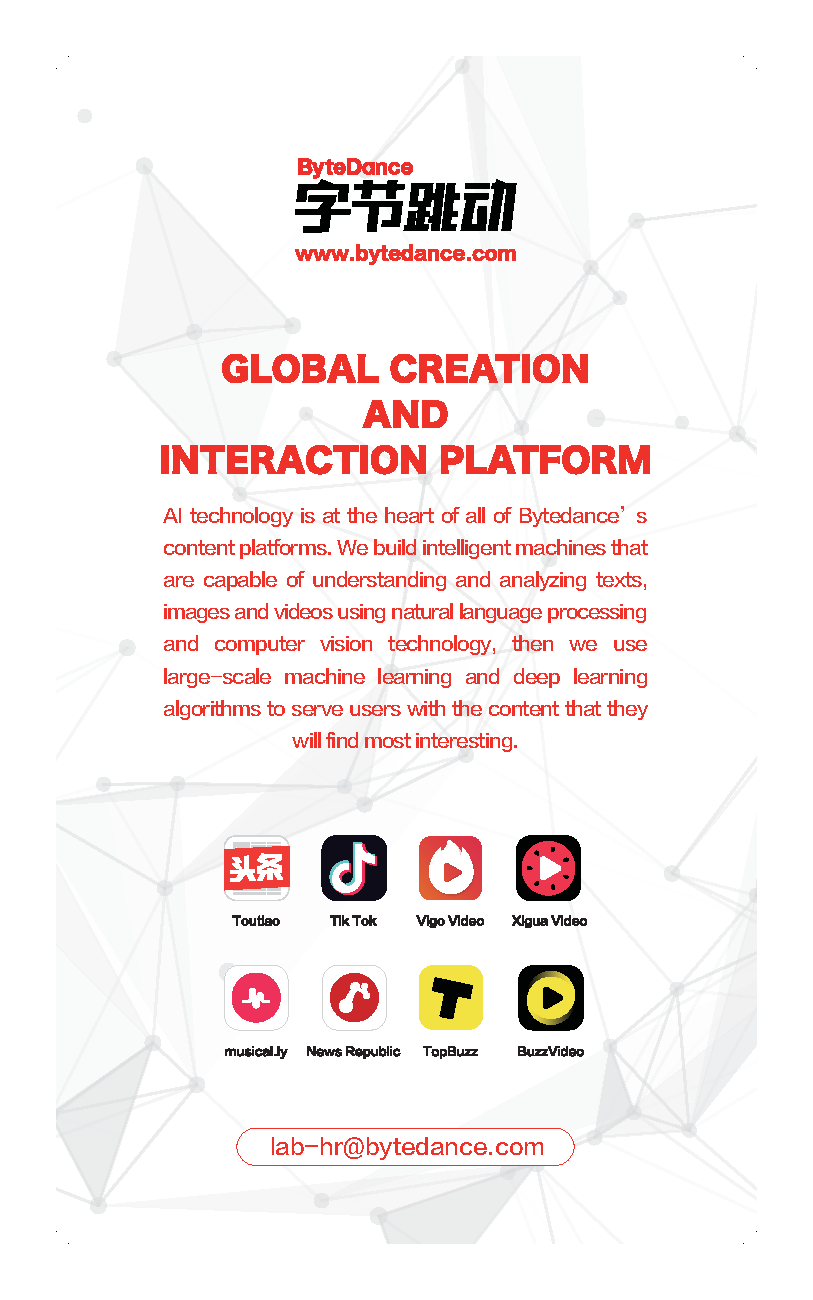
\includepdf[pages={1}]{content/ads/diamond/bytedance}

\includepdf[pages={1}]{content/ads/diamond/bloomberg}

\includepdf[pages={1}]{content/ads/platinum/amazon}

% Gold sponsors
\includepdfmerge[nup=1x2]{content/ads/Gold/capitalone, 1, {content/ads/Gold/ignite.jpg}, 1}

\includepdfmerge[nup=1x2]{content/ads/Gold/grammarly, 1, {content/ads/Gold/twosigma}, 1}


\includepdfmerge[nup=1x2]{content/ads/Gold/tulane, 1, content/ads/Gold/polyai, 1}

\includepdfmerge[nup=1x2]{content/ads/Gold/ibm, 1}%, {content/ads/Gold/ibm}, 1}

% put grammarly with crochet
%\includepdfmerge[nup=1x2]{content/ads/Gold/oracle, 1, {content/ads/Gold/crochet}, 1}


% Silver and Bronze sponsors
\includepdfmerge[nup=2x2]{content/ads/Silver/nuance, content/ads/Silver/facebook, content/ads/Silver/isi}
%\includepdfmerge[nup=2x2]{content/ads/Silver/facebook, content/ads/Silver/facebook, content/ads/Silver/facebook, content/ads/Silver/facebook}
% \includepdfmerge[nup=1x2]{content/ads/Silver/01-Adobe_resized+Gold, content/ads/Silver/02_03-Bosch+CVTE_resized}
% \includepdfmerge[nup=2x2]{content/ads/Silver/04-duolingo_resized, content/ads/Silver/05-Huawei_resized, content/ads/Silver/06-Nuance_resized, content/ads/Silver/07-Sogou_resized}

% \iftranslatorad
% \includepdfmerge[nup=2x2]{content/ads/Silver/08-Oracle_resized, content/ads/Bronze/01-Grammarly_resized, content/ads/Bronze/02-Toutiao_resized, content/ads/Translator}
% \else
% \includepdfmerge[nup=2x2]{content/ads/Silver/08-Oracle_resized, content/ads/Bronze/01-Grammarly_resized, content/ads/Bronze/02-Toutiao_resized, content/ads/EmptyAd}
% \fi

% \else

% % Platinum sponsors
% 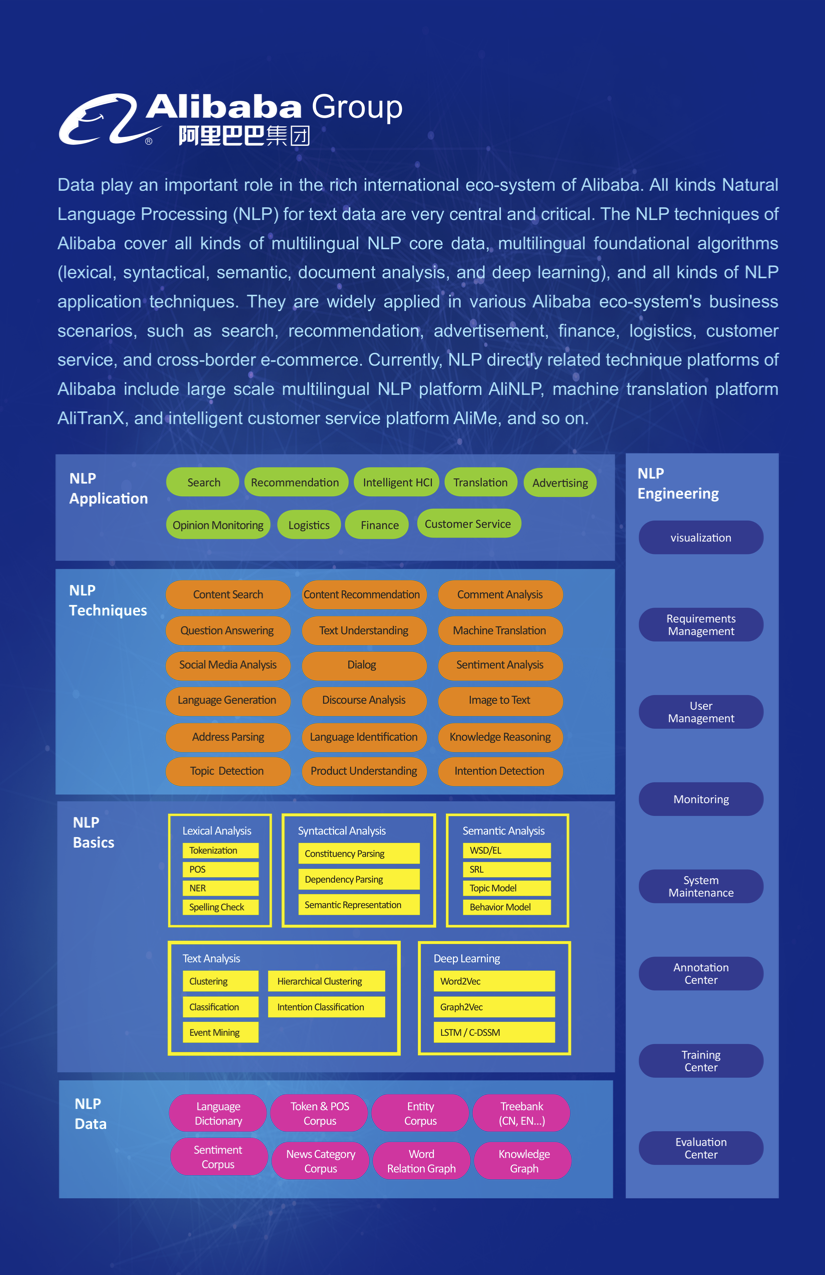
\includepdf[pages={1}]{content/ads/Platinum/01-Alibaba_resized_small.png}
% 
\includepdf[pages={1}]{content/ads/Platinum/02-amazon_resized_small.png}
% 
\includepdf[pages={1}]{content/ads/Platinum/03-Baidu_resized_small.png}
% 
\includepdf[pages={1}]{content/ads/Platinum/04-Bloomberg_resized_small.png}
% 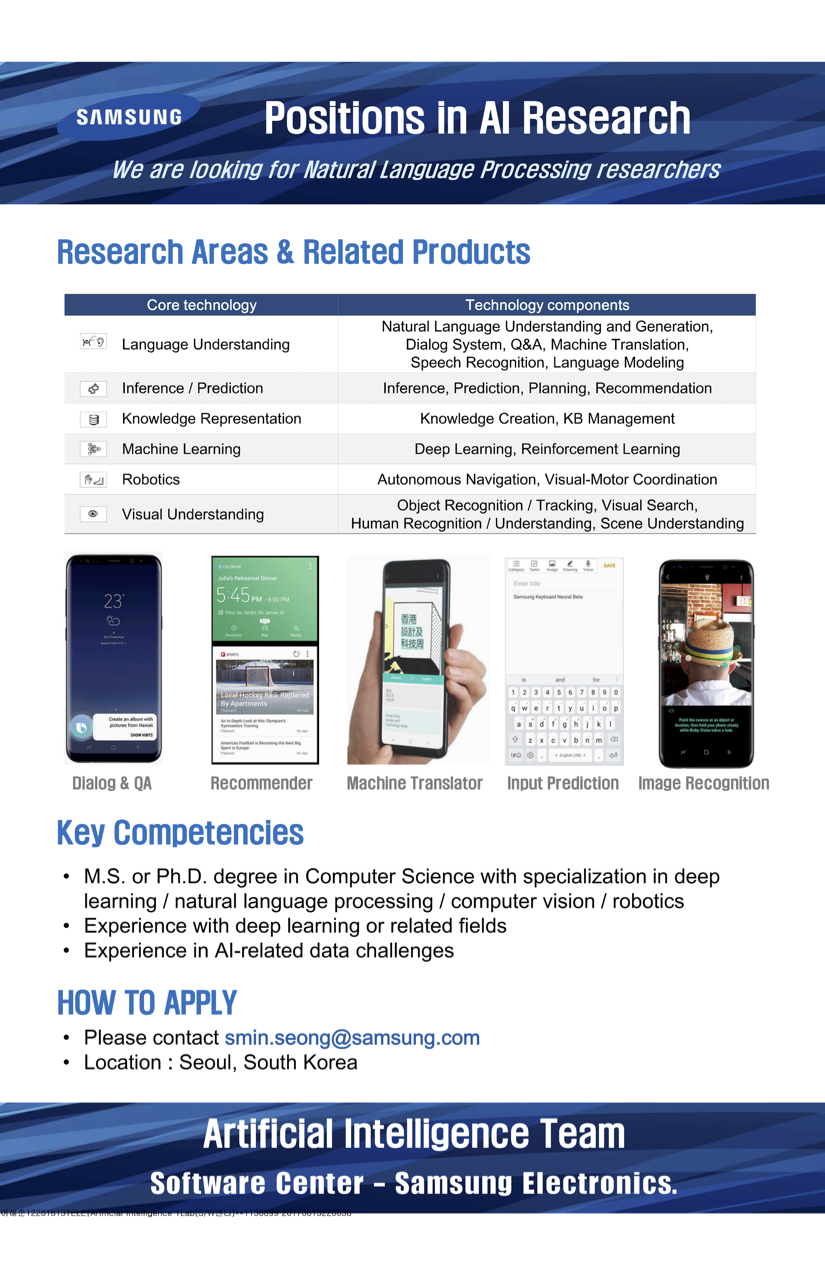
\includepdf[pages={1}]{content/ads/Platinum/05-Samsung_resized_small.png}
% 
\includepdf[pages={1}]{content/ads/Platinum/06-Tencent_resized_small.png}

% % Gold sponsors
% \includepdfmerge[nup=1x2]{content/ads/Gold/01-eBay_resized_small.png, 1, content/ads/Gold/02-Elsevier_resized_small.png, 1}
% \includepdfmerge[nup=1x2]{content/ads/Gold/03-KPMG_resized_small.png, 1, content/ads/Gold/04-Maluuba_resized_small.png, 1}
% \includepdfmerge[nup=1x2]{content/ads/Gold/05-SAP_resized_small.png, 1, content/ads/Gold/06-IBM_resized_small.png, 1}
% \includepdfmerge[nup=1x2]{content/ads/Gold/07-RIT_resized_small.png, 1, content/ads/Gold/08-NaverCorp_resized_small.png, 1}
% \includepdfmerge[nup=1x2]{content/ads/Gold/09-NEC_resized_small.png, 1, content/ads/Gold/10-MSFT_resized_small.png, 1}

% % Silver and Bronze sponsors
% \includepdfmerge[nup=1x2]{content/ads/Silver/01-Adobe_resized+Gold_small.png, content/ads/Silver/02_03-Bosch+CVTE_resized_small.png}
% \includepdfmerge[nup=2x2]{content/ads/Silver/04-duolingo_resized_small.png, content/ads/Silver/05-Huawei_resized_small.png, content/ads/Silver/06-Nuance_resized_small.png, content/ads/Silver/07-Sogou_resized_small.png}
% \includepdfmerge[nup=2x2]{content/ads/Silver/08-Oracle_resized_small.png, content/ads/Bronze/01-Grammarly_resized_small.png, content/ads/Bronze/02-Toutiao_resized_small.png, content/ads/Translator}

% \fi

\clearpage


%% BACK COVER %%%%%%%%%%%%%%%%%%%%%%%%%%%%%%%%%%%%%%%%%%%%%%%%%%%
\fancyfoot[C]{}
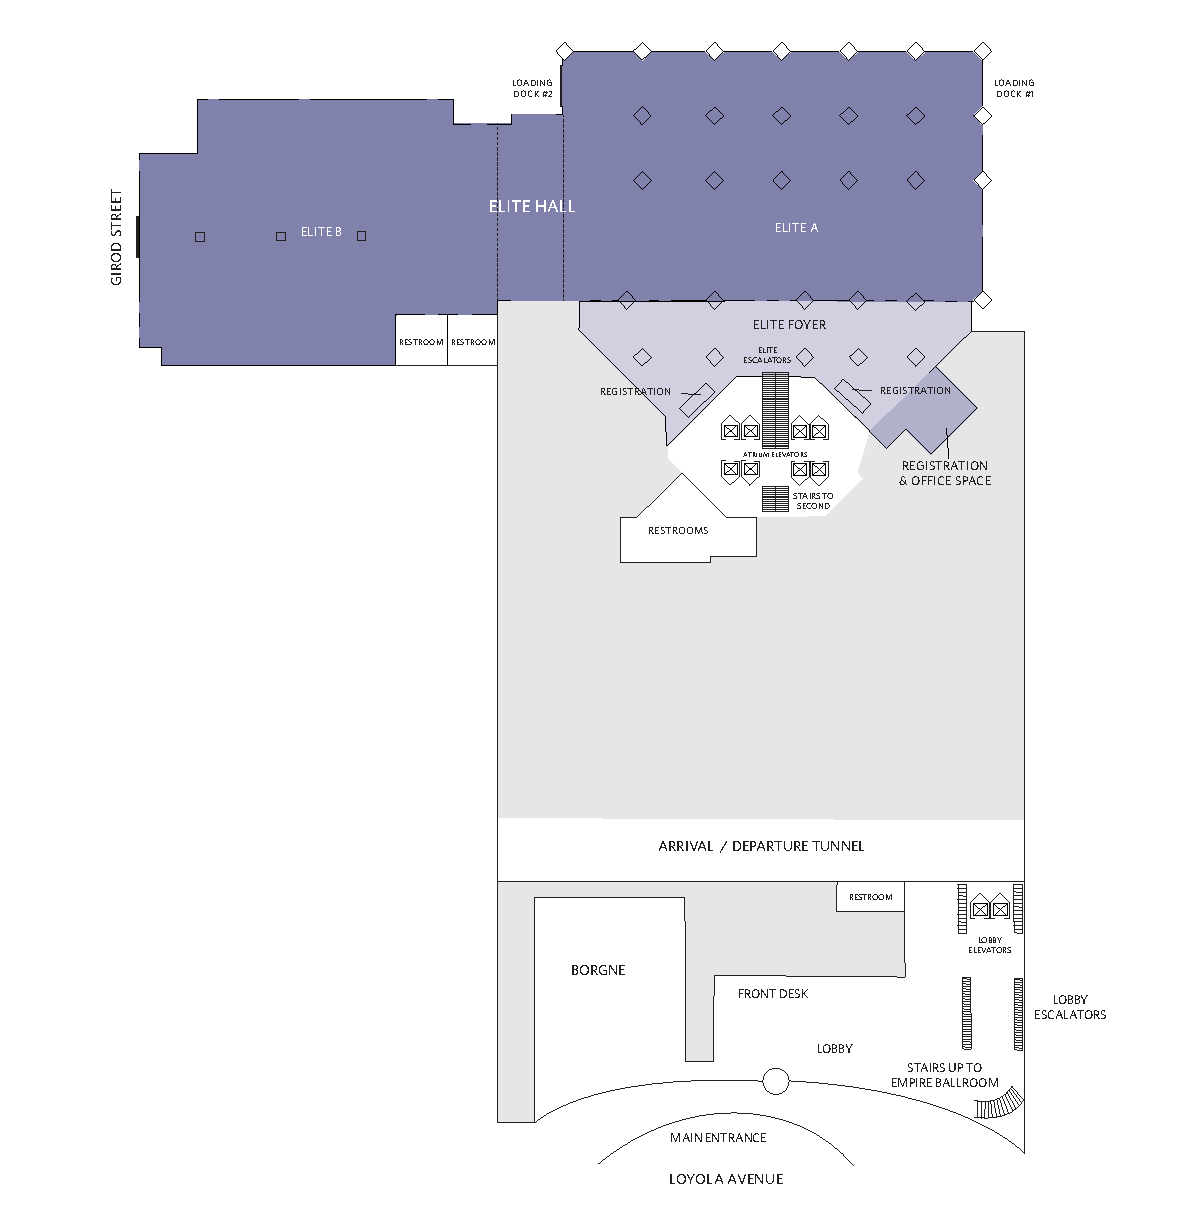
\includepdf[pages={1-2},nup={1x2}]{content/fmatter/2018-NAACL-Hyatt-Regency-New-Orleans-Floor-Plans-4242018}

\includepdf[pages={1}]{content/fmatter/back.pdf}

\end{document}
